% VIGTIGT! For at dokumentet kan compile, skal man benytte XeLaTeX eller LuaLaTeX som compiler. Dette kan gøres i Overleaf ved at gå til Menu -> Settings -> Compiler -> Vælg XeLaTeX/LuaLaTeX
\documentclass[12pt]{article}
\usepackage{KUstyle}
\usepackage[margin=0.8in]{geometry} % Pakke til sidemargin
\usepackage{setspace} % Pakke til halvanden linjeafstand
\usepackage{tabularx} % Pakke til tabel
\usepackage{fontspec}
\usepackage{mathtools} % til at skrive matematiske symboler
\usepackage{amsmath} % bruges til ligninger og matematik
\usepackage{amssymb} % symboler og andre ting og sager
\usepackage{graphicx} % inkluderer grafik og specielle grafiske modulatorer
\usepackage{float} % inkluderer float som en konfiguerations enhed
\graphicspath{{./images/}} % stien til billeder
\usepackage{natbib} % bibliografi.bst style config
\bibliographystyle{jmr} % bibliografi stilen. denne stil laver (navn, dato). Dokumentation findes i jmr.bst
\usepackage[danish]{babel} % en pakke til dansk, så labels er på dansk
\usepackage{xltxtra} % til at skrive sub- og superscripts
\usepackage{times}
\usepackage{gensymb} % symbolpakke
\usepackage{hyperref} % referencer
\usepackage{array} % til tabeller
\usepackage[table, xcdraw]{xcolor} % til tabeller
\usepackage{longtable} % til tabeller
\usepackage{caption} % til captions
\usepackage{multirow} % til tabeller 
\usepackage{subcaption} % til tabeller
\usepackage{colortbl} % til tabeller
\usepackage{makecell} % til tabeller
\usepackage{booktabs} % til tabeller
\usepackage[normalem]{ulem}
\useunder{\uline}{\ul}{}
\usepackage{xurl}
\usepackage{wrapfig}
\usepackage{subcaption}
\usepackage{minted} % til kode
\usepackage{tabularray}
\UseTblrLibrary{diagbox}
\usepackage{booktabs,siunitx,array,threeparttable}
\usepackage{diagbox}
\usepackage{setspace}



\setlength{\bibhang}{2em}



\hypersetup{breaklinks, colorlinks, urlcolor=black
}

\captionsetup[figure]{font=small,labelfont=bf, labelsep=period}
\captionsetup[figure]{justification=l, singlelinecheck=false}
\captionsetup[subfigure]{font=footnotesize, labelfont=bf, justification=centering}
\captionsetup[table]{font=small, labelfont=bf, labelsep=period}
\captionsetup[table]{justification=l,singlelinecheck=false}




\tolerance=1
\emergencystretch=\maxdimen
\hyphenpenalty=10000
\hbadness=10000

\setmainfont{Times New Roman}
\setlength{\parindent}{0pt}



% Nedenstående ændrer indholdet på forsiden
\ptype{Bachelorprojekt i geografi og geoinformatik}
\author{Johan Bo Kjær}
\title{Titel}
\subtitle{Undertitel}
\date{Dato: {\today}}
\advisor{Vejleder: Mikkel Fruergaard}
\fpimage{bil.jpg} % Hvis intet billede ønskes, skal kommandoen fjernes
\fpcredit{Aabenraa midtby under stormfloden i oktober 2023. Kredit: Meks I/S}


\begin{document}


\maketitle


\onehalfspacing


\begin{table}[h]
\def\arraystretch{1.5}
\begin{tabularx}{\textwidth}{l X}
Institutnavn: & {Institut for Geovidenskab og Naturforvaltning}  \\
Forfatter: & {Johan Bo Kjær} \\
KU-brugerID: & {MCG811} \\
Titel og evt. undertitel: & {Titel, evt. undertitel} \\
Emnebeskrivelse: & Lorem ipsum dolor sit amet, consectetur adipiscing elit. Vestibulum porttitor rhoncus dui, vehicula pellentesque odio convallis id. Vestibulum mollis nulla ut sem luctus dictum. Sed scelerisque feugiat arcu, quis faucibus lorem viverra id. Aenean dignissim metus eu ligula sagittis, at commodo magna suscipit. \\
Nøgleord: & GIS-modellering, klimaforandringer, kyst, oversvømmelse, stormfloder \\
Vejleder: & Mikkel Fruergaard \\
Dato: & \today \\
Afleveringsdato: & 4. juni 2025 \\
Antal anslag: &  \\
Totale antal sider: & \\
Tak til: & Aabenraa, Guldborgsund og Vordingborg kommune for adgang til data \\
& kgdflg
\end{tabularx} 
\end{table}

% begin: renewcommands:
\renewcommand{\contentsname}{Indholdsfortegnelse} % ændrer navnet på indholdsfortegnelsen
\renewcommand{\abstractname}{Abstract} %nanvet på abstract
\renewcommand{\refname}{} % sørger for at der ikke er en ekstra titel i referencelisten.

% end: renewcommands:

\newpage
% her er en begyndelse det engelske del af resumeét
\begin{table}[h]
\def\arraystretch{1.5}
\begin{tabularx}{\textwidth}{l X}
\LARGE{Project title:} & \LARGE{Titel på afhandling, evt. undertitel} \\
Author: & {Johan Bo Kjær} \\
Keywords: & \textit{climate change, coastal, GIS-modelling, inundation, storm surge}
\end{tabularx}
\end{table}
\begin{abstract}
    Lorem Ipsum dominus scripticus
\end{abstract}

\newpage

\tableofcontents
\newpage


\section{Introduktion}



\section{Teori}

%UKDAST!!!!!!!!!!!!!!!!!!!!!!!!!!!!!!!!!!!
\subsection{Raster datamodel} \label{Afsnit: Raster data model}

En rastermodel er en datamodel der er bygget op af et regulært netværk af celler organiseret i et gitterformat \citep{bolstad_gis_2022, esri_raster}. Hver celle i en raster model er karakteriseret af en celle dimension, som definerer cellestørrelsen ud fra cellens længde i X- og Y-retningen \citep{bolstad_gis_2022, silbernagel_raster_2018}. Cellestørrelsen repræsenterer således den rumlige opløsning af raster datamodellen og fungerer som en indikator for den rumlige præcision, da hver celles koordinat er givet ud fra centrum af cellen. En større cellestørrelse vil derfor resultere i en højere rumlig usikkerhed, mens en mindre cellestørrelse vil medføre en lavere rumlig usikkerhed \citep{bolstad_gis_2022}. \\

Hver celle i en raster indeholder en værdi, der repræsenterer information. Denne information kan enten kan være numerisk eller kategoriske. Numeriske værdier anvendes ofte til at repræsentere kontinuerlige data, såsom højdeinformationer i en højdemodel (figur \ref{Subfig: Kontinuer raster}), mens kategoriske værdier anvendes ved diskret og tematiske data, såsom arealklasser (figur \ref{Subfig: Kategorisk raster}). 
\begin{figure}[H]
    \begin{subfigure} [t]{0.5\textwidth}
        \centering
        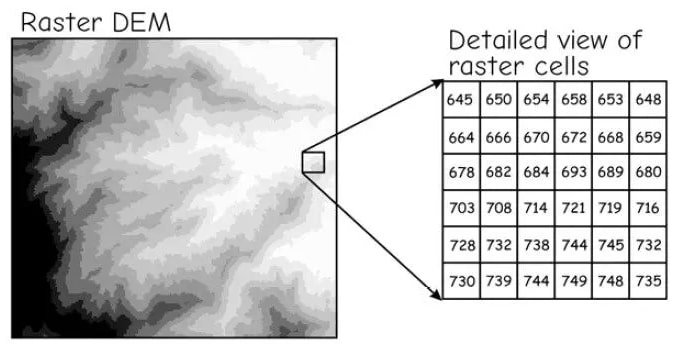
\includegraphics[width=1\linewidth]{images/teori/raster_kontinuert.jpg}
        \caption{}
        \label{Subfig: Kontinuer raster}
    \end{subfigure}
    \begin{subfigure} [t]{0.5\textwidth}
        \centering
        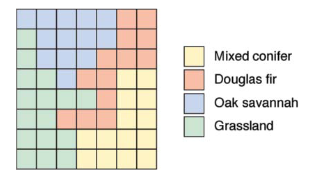
\includegraphics[width=1\linewidth]{images/teori/raster_areal.png}
        \caption{}
        \label{Subfig: Kategorisk raster}
    \end{subfigure}
    \caption{Eksempel på en raster med numeriske kontinuert data fra en højdemodel \textbf{(a)} og en kategorisk raster med diskrete data over arealanvendelse \textbf{(b)}. Kilde: \cite[s. 66]{bolstad_gis_2022} og \cite[s. 67]{longley_geographical_2008}}
    \label{Figur: Kontinuert og kategorisk raster}
\end{figure}

Rastermodellens struktur muliggør omfattende rumlig analyse, idet der kan udføres artimetiske og logiske operationer på tværs af celler og mellem flere forskellige rasterlag. Denne egenskab gør det derfor også muligt at analysere og kombinere kontinuerte og diskrete rumlige informationer i et GIS-miljø \citep{bolstad_gis_2022, longley_geographical_2008}.

\subsection{Inundation Modellen} \label{Afsnit: Inundation Model}

Til projektet er der blevet anvendt en GIS-baseret stormflods model kaldet \textit{"Inundation Model"} udarbejdet af \cite{balstrom_kirby_inundation} til at give et bud på hvordan en stormflod vil påvirke et område. Modellen opererer eksklusivt i et ArcGIS Pro miljø, GIS-softwaren udviklet af Esri.\\
Modellen indeholder en række værktøjer, der bruges til at analysere stormfloders påvirkning af et område og kernen i modellen er værktøjet \textit{"Create Inundation"} som er en statisk numerisk rastermodel. Modellen benytter tre brugerdefineret parametre der består af tre numeriske værdier i meter: InitialSealLevel, SeaLevelIncrement og Number of Iterations. Modellen benytter også en hydrologisk korrigeret Digital Terræn Model (DHyM) og en bruger digitaliseret linjeobjekt som kilde for udregningen, benævt Line at Sea \citep{balstrom_kirby_inundation}. I figur \ref{Figur: Create Inundation} er modellens opbygning vist inddelt i to segmenter.

\begin{figure}[H]
    \centering
    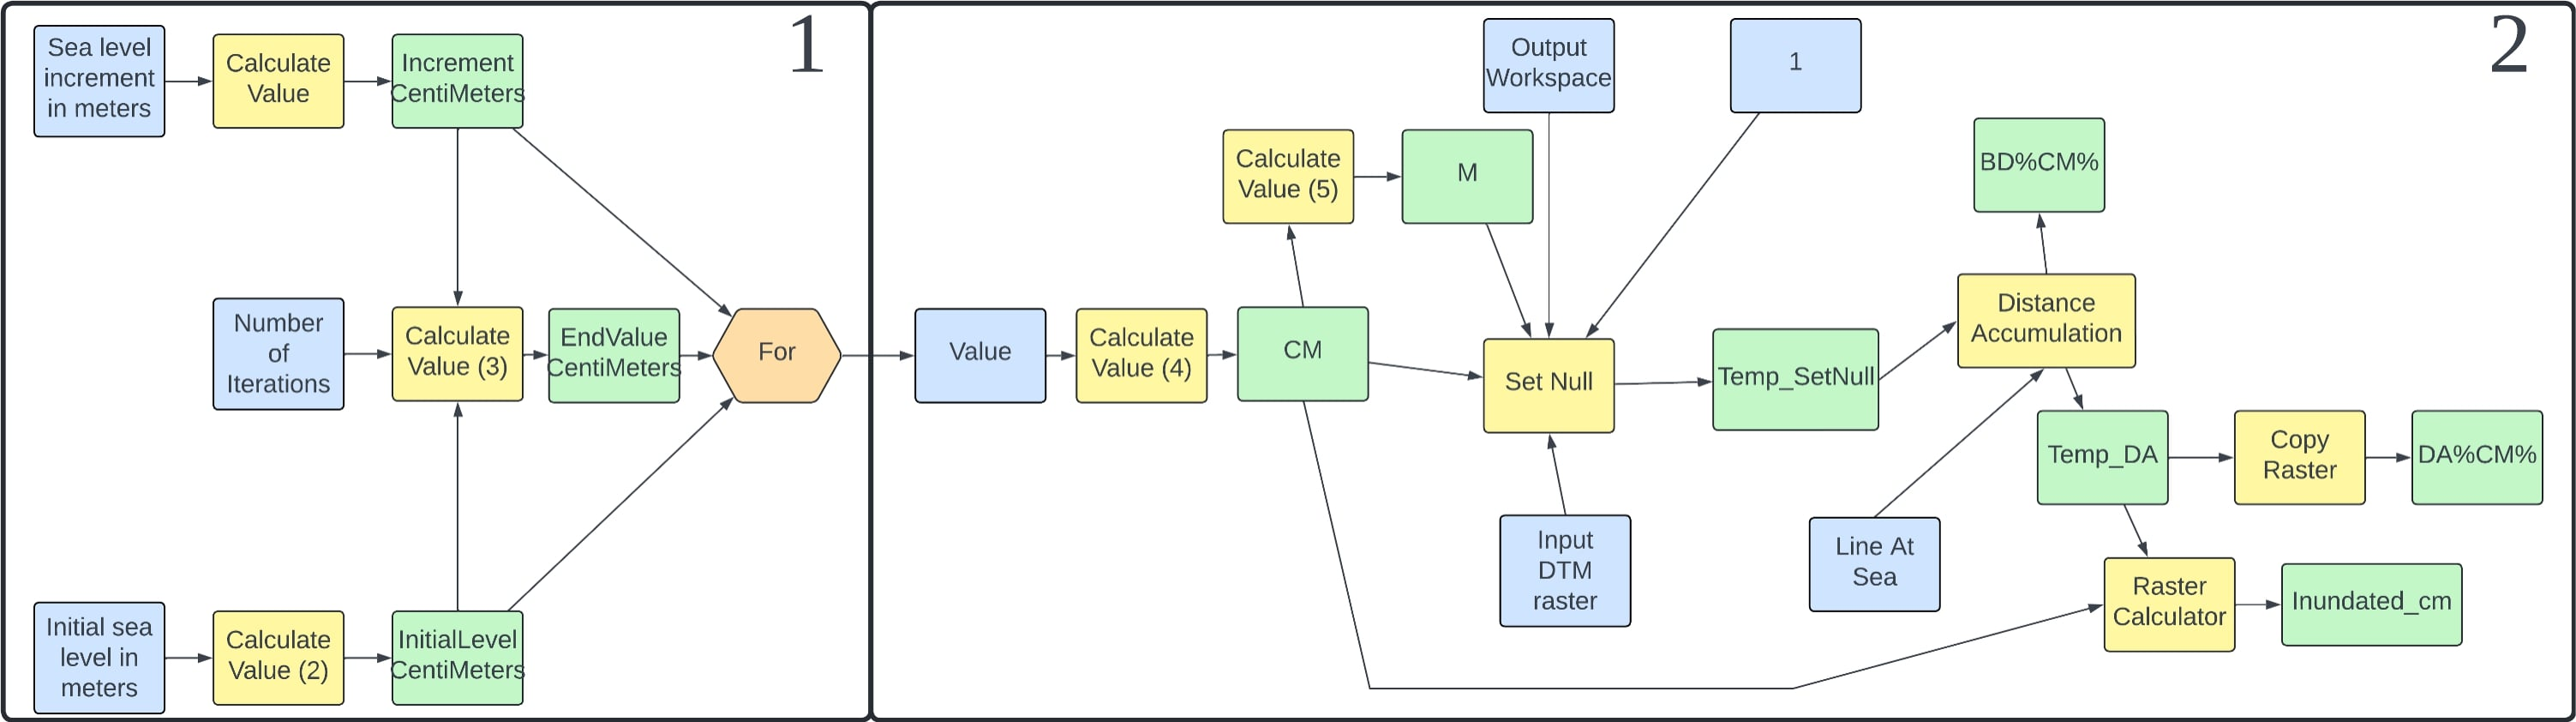
\includegraphics[width=1\linewidth]{images/teori/inundation_model_separated.jpg}
    \caption{Flowchart af Inundation Modellens \textit{"Create Inundation"} værktøj.}
    \label{Figur: Create Inundation}
\end{figure}

Det første segment er en omregning af brugerens input i meter til centimeter for både stigningsniveauet for hver gang modellen itererer og det begyndende havniveau. Modellen kræver en afsluttende værdi for hvornår den skal stoppe med at iterere. Denne værdi svarer til den vandstand der ønskes at simulere op til. Denne værdi bliver udregnet ved følgende: $InitialSeaLevel + ((NumberIterations - 1)\times Increment)$. \\

Det andet segment af modellen er selve oversvømmelses beregningen gennem terrænet. Det starter med et for-loop der starter med den første værdi (fx 100 cm). Denne værdi omregnes tilbage til meter hvorefter modellen eksekverer et tjek (figur \ref{Figur: Create Inundation} "SetNull") på cellerne i DTM. Her tjekkes alle celleværdierne i DTM for om de er større eller ligmed den nuværende værdi. Hvis dette hvis-ellers tjek er sandt bliver cellerne tildelt NoData værdien, som indikerer at cellen ikke bliver oversvømmet ved dette oversvømmelsesniveau. Hvis DTM celleværdien er lavere end tjekværdien og udtrykket dermed er falsk bliver cellen angivet med et 1, som indikerer at den bliver oversvømmet ved det niveau (figur \ref{Figur: Celler Inundated}).       

\begin{figure}[H]
    \centering
    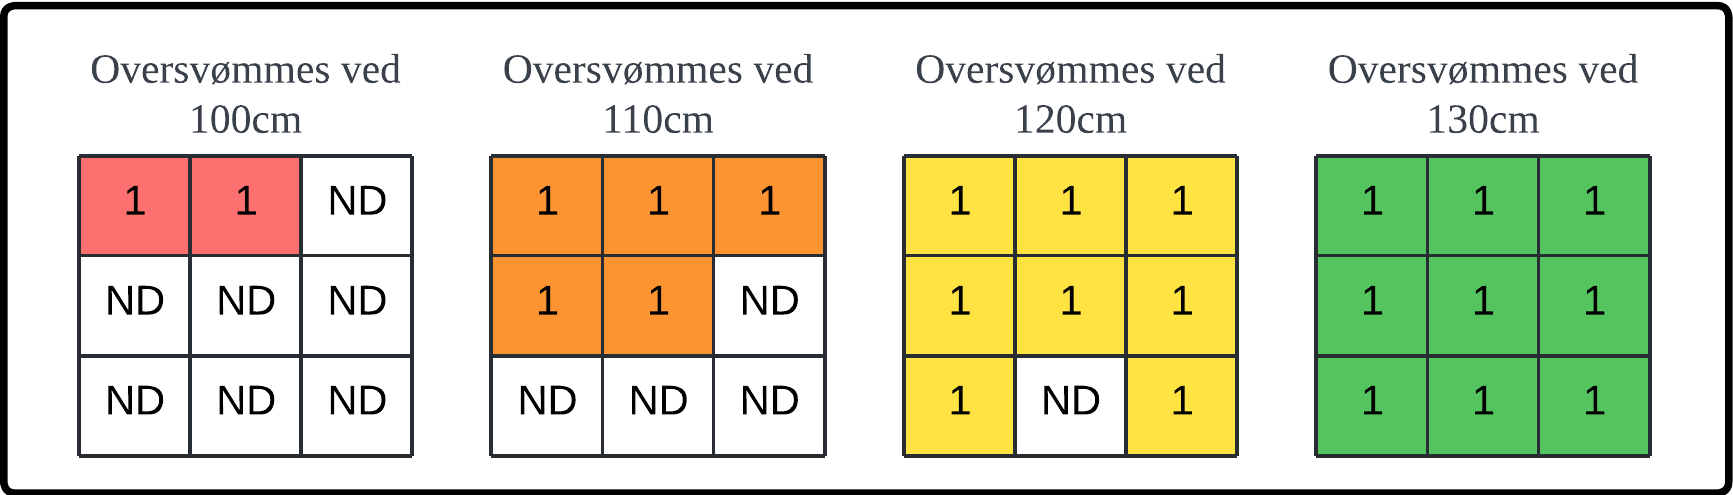
\includegraphics[width=0.7\linewidth]{images/teori/celler_inundated.png}
    \caption{Princippet bag Inundation Modellen gennem raster celler. 1 angiver at cellen oversvømmes ved det pågældende niveau og ND = NoData (celler som ikke bliver oversvømmet).  Egen illustration med inspiration fra \cite{balstrom_kirby_inundation}}.
    \label{Figur: Celler Inundated}
\end{figure}

Herefter udføres en Distance Accumulation igennem de celler der bliver oversvømmet ved det bestemte niveau fra en linjekilde. En Distance Accumulation er en analysemetode der beregner den samlede afstand fra en kilde ud igennem et område \citep{esri_how_nodate}. I Inundation modellen bliver Distance Accumulation brugt til at efterligne vandets bevægelse igennem cellerne på samme måde som vandet ville sprede sig under en stormflod. Distance Accumulation vil sprede sig igennem terrænet indtil en ufremkommelig barriere er mødt.\\ 
Distance Accumulation starter fra linjen \textit{"Line at Sea"} og bevæger sig igennem alle cellerne i terrænet hvor cellen = 1. Hvis cellen er NoData så kan vandet ikke bevæge sig igennem \citep{balstrom_kirby_inundation}. Resultatet af Distance Accumulationen bliver derefter koblet med det oversvømmelsesniveau der bliver itereret over for at give resultatet af modellen.  


\subsection{Stormfloder i Danmark} \label{Afsnit: Stormfloder}

En stormflod betegner en markant forhøjet vandstand langs kysten, der primært opstår som følge af kraftigt stormvejr \citep{shoreline_management_guidelines}. Stormfloder dannes typisk i en kombination af flere faktorer: vindstuvning presser havvand ind imod kysten, bølgepåvirkning kan forstærke vindstuvningen, lavere atmosfærisk tryk medfører en lokal stigning i vandstand, og i områder med tidevand kan en stormflod forstærkes yderligere, hvis højvande sammenfalder med en stormflod \citep{piecuch_high-tide_2022}. Derudover er en stormflods intensitet og indvirkning på en lokalitet afhængig af andre lokale forhold herunder kystens orientering i forhold til vindretningen samt havbundens og kystens morfologi \citep{noaa_storm, shoreline_management_guidelines}.\\

I Danmark er det Vadehavs- og vestkysten af Jylland der er det mest udsatte område, da vinden i Danmark primært kommer fra vest \citep{cappelen_dmi_2020}, men den sydlige del af Danmark er også et udsat område. Over længere perioder med vesten vind, vil vandet i Nordsøen gradvist blive presset ind Kattegat og længere ned i de indre danske farvande. Hvis en vestlig vind er langvarig, vil vandet over tid blive presset igennem bælterne ved Lillebælt, Storebælt og Øresund og videre ind i Østersøen og nord imod den Botniske Bugt \citep{kiesel_brief_2024, egusphere_baltic}. Dette fænomen kaldes for \textit{"preconditioning"} og beskriver hvordan vandstanden stiger i Østersøen inden begyndelsen af en storm \citep{kiesel_brief_2024, weisse_sea_2021}. \\   

Når vinden derefter aftager eller ændres til østenvind vil ophobet vandet der er blevet presset ind i Østersøen, strømme tilbage mod bælterne i Danmark. Dette kaldes for \textit{"badekarseffekten"} og er illustreret i figur \ref{Figur: Bathtub effect} \citep{kystdirektoratet_stormfloder, egusphere_baltic}. Bælterne i de indre danske farvande vil herefter fungere som flaskehalse for vandmasserne der skvulper tilbage fra Østersøen og resultere i oversvømmelse i de indre danske farvande samt andre fjorde og bugter i Nordtyskland \citep{egusphere_baltic}.
\begin{figure}[H]
    \centering
    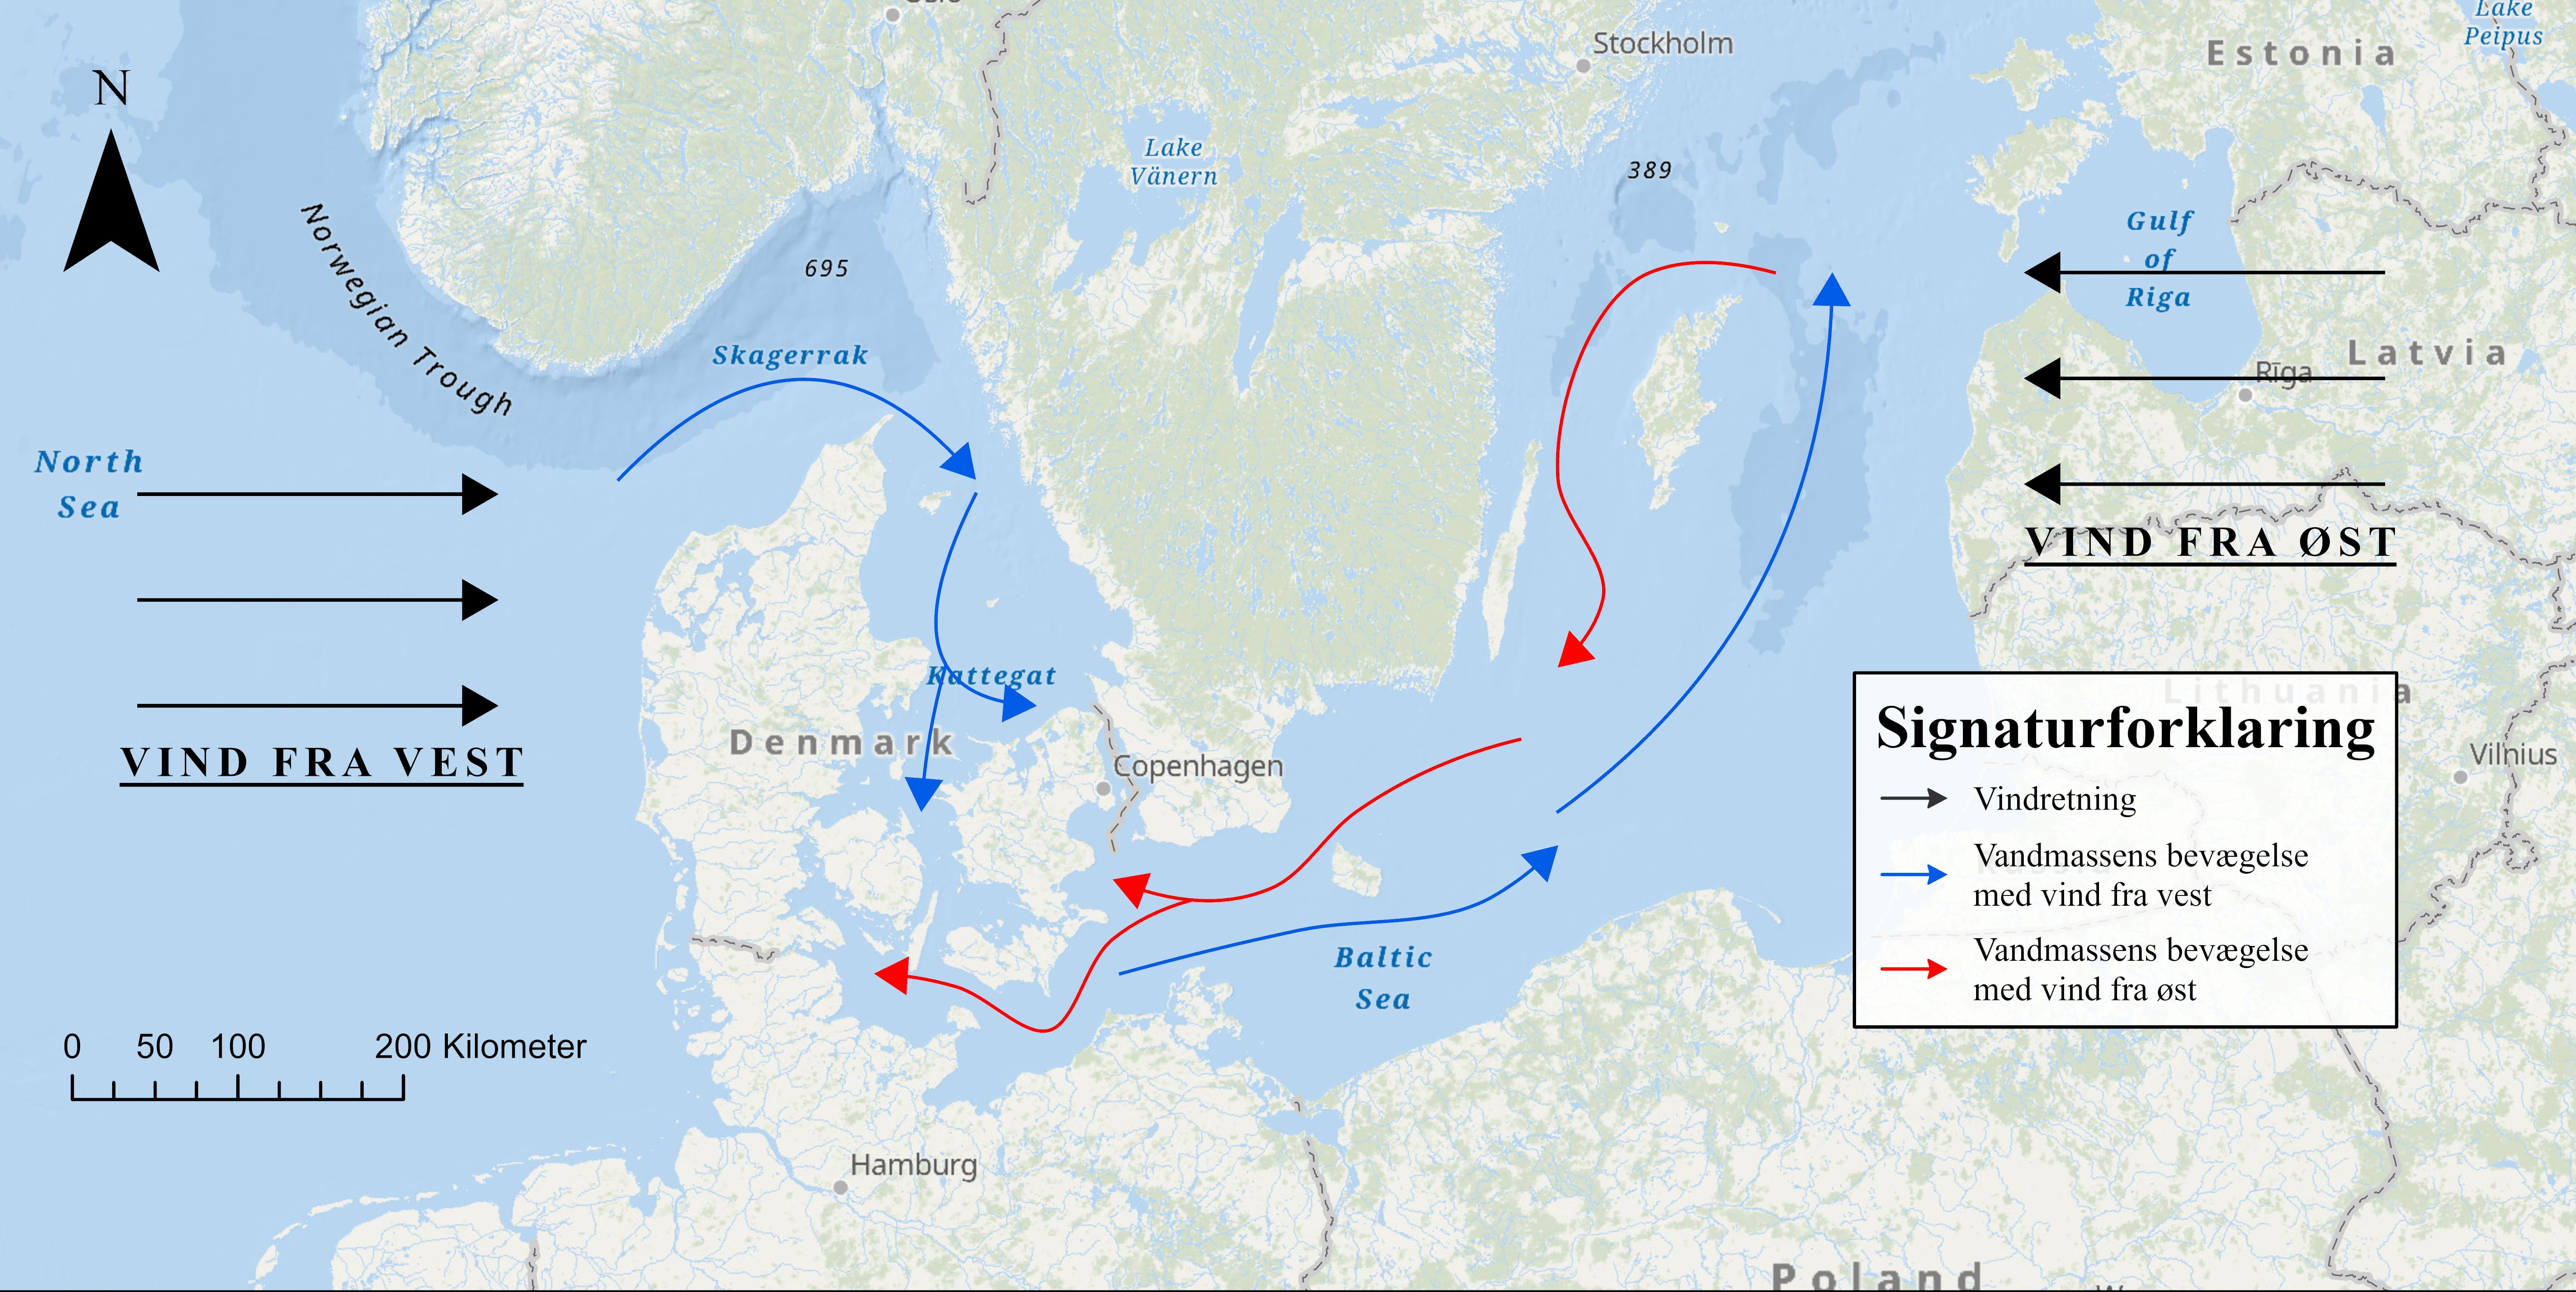
\includegraphics[width=0.8\linewidth]{images/teori/bathtub effect graphics.jpg}
    \caption{Illustration af badekarseffekten i Østersøen. De sorte pile indikerer vindretning og de blå og røde pile indikerer bevægelsen af vandmassen ved henholdsvis vest- og østenvind. Kilde: Egen illustration, baggrundskort fra Esri}
    \label{Figur: Bathtub effect}
\end{figure}

Historisk har flere betydelige stormfloder i Danmark, såsom stormfloderne i november 1872, november 2006 and oktober 2023, været forårsaget af en kombination af længerevarende vestenvind efterfulgt af østenvind og den resulterende badekarseffekt \citep{kystdirektoratet_stormfloder}.

\subsection{Stormfloden den 20 oktober 2023} \label{Afsnit: Stormfloden den 20 oktober 2023}
I første halvdel af oktober 2023 blev der observeret moderate vindforhold med gennemsnitlig middelvind på 5,5 m/s og en gennemsnitlig maksimal 10.min middelvind på 18,3 m/s fra vest, hvilket medførte en betydelig vandtransport ind gennem Kattegat og videre i Østersøen \citep{dmi_vejrarkiv}. \\
Den 18. oktober skiftede vindretningen til øst (figur \ref{Figur: Vinddata Danmark}) grundet trykforskelle mellem et højtryksystem over Skandinavien og et lavtrykssystem over Storbritannien \citep{kiesel_brief_2024}, og middelvindhastigheden steg i hele landet til 12,2 m/s og maksimale 10.min middelvind til 28,3 m/s om aftenen den 20. oktober 2023. 
\begin{figure} [H]
    \centering
    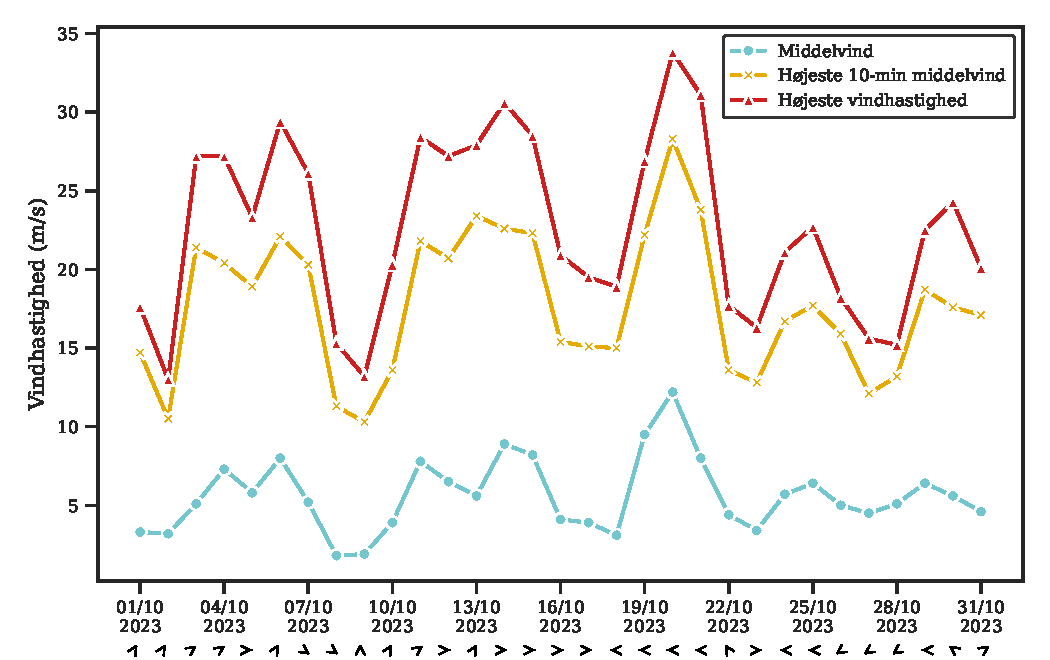
\includegraphics[width=0.8\linewidth]{images/teori/vinddata_grafer/Danmark_vinddata.pdf}
    \caption{Vinddata for Danmark i oktober 2023 der viser middelvind, højeste 10.min middelvind og højeste vindhastighed i m/s. De sorte pile i bunden indikerer vindretningen. Kilde: Data fra \cite{dmi_vejrarkiv} }
    \label{Figur: Vinddata Danmark}
\end{figure}

Kombinationen af kraftig vind fra øst og stor vandtransport ind i Østersøen over en periode på 15 dage resulterede ifølge \cite{kystdirektoratet_stormflod2023} i markante vandstandsstigninger i de indre farvande af Syddanmark i løbet af eftermiddagen den 20. oktober. Den højeste officielle vandstand målt under stormfloden blev målt i Aabenraa Havn på 2,16 m over dagligt vande \citep{damberg_vaerste_2023}. Disse forhold forårsagede omfattende skader af sommerhusområder, kystnære områder og byer \citep{kystdirektoratet_stormflod2023, naturskaderadet_anmeldelser_2023}. 








\section{Studieområder}

I projektet er der blevet arbejdet på fire studieområder i Danmark. De fire studieområder er Aabenraa, Gedser Havn, Hesnæs og Præstø.\\

Til udvælgningen af studieområderne blev i alt otte kommuner kontaktet. Dette inkluderer Aabenraa, Faaborg-Midtfyn, Guldborgsund, Haderslev, Stevns, Sønderborg og Vordingborg. Denne udpegning af potentielle lokaliteter skete på baggrund af en tabel fra \cite{damberg_vaerste_2023} over højeste målte vandstande i Danmark under oktober 2023 stormfloden. 
Ud af de otte kommuner blev tre kommuner (Aabenraa, Guldborgsund og Vordingborg) udvalgt til videre samarbejde på baggrund af tilgængeligt data. Guldborgsund kommune stillede data fra fire lokaliteter i kommunen til rådighed og der blev udvalgt de to kystbyer, Gedser Havn og Hesnæs, på baggrund af højere målt vandstand under stormflode i oktober 2023. \\

De fire udvalgte studieområder er lokaliseret langs sydkysten af Danmark. På figur \ref{Figur: Oversigtskort} er områdernes placering i Danmark visualiseret. Alle fire lokaliteter oplevede forhøjet vandstand under stormfloden den 20.-21. oktober 2023. 
\begin{figure}[H]
    \centering
    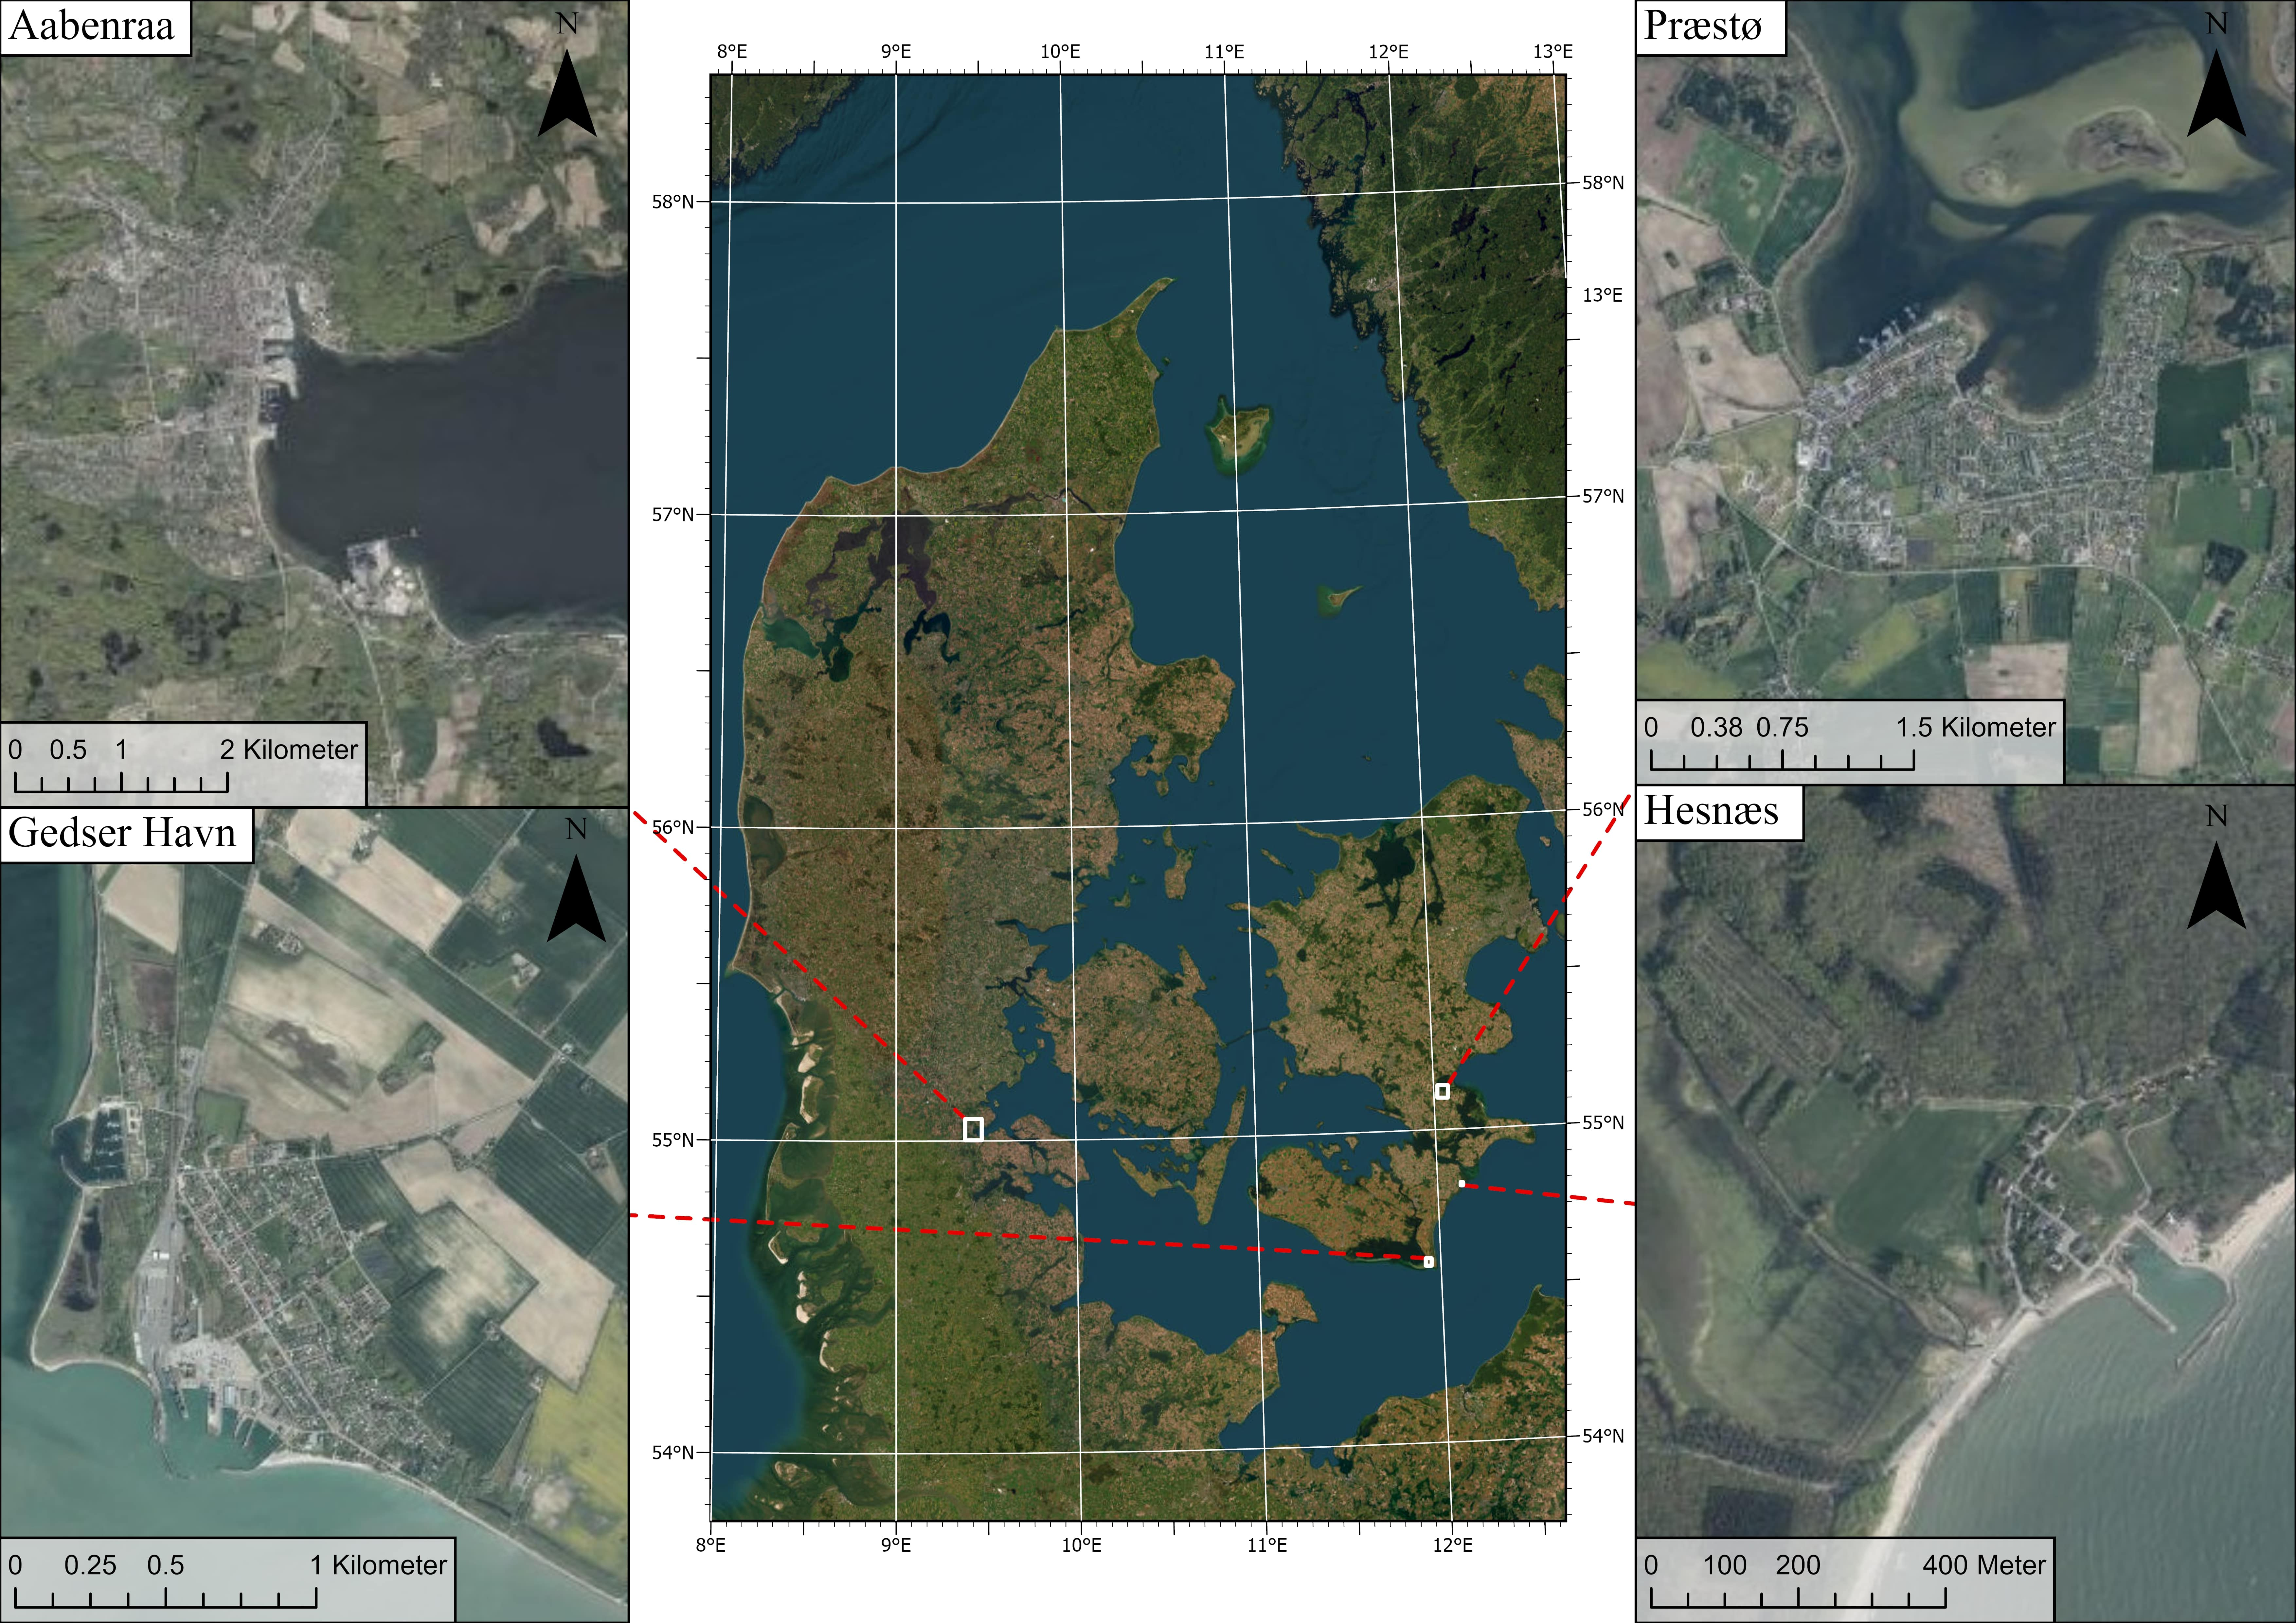
\includegraphics[width=1\linewidth]{images/studieområder/oversigtskort.jpg}
    \caption{Oversigtskort over studieområderne: Aabenraa, Gedser Havn, Hesnæs og Præstø. Baggrundskort fra ESRI og Klimadatastyrelsen}
    \label{Figur: Oversigtskort}
\end{figure}

Aabenraa er en by i det sydøstlige Sønderjylland. Byen er beliggende i Aabenraa kommune for enden af den ca. 10 km lange Aabenraa fjord. Byen har en befolkning på 16500 og er den niende største by i Region Syddanmark \citep{danmarks_statistisk_mobile_nodate}. Byen består af to store industri havne, Aabenraa og Ensted, og er en vigtigt for skibstrafik med 380 anløbte skibe i 2022 \citep{aabenraa_havn_aabenraa-havn-talogfakta2022_2022}.\\
Aabenraa oplevede den højeste officielle måling af vandstand under stormfloden den 20.-21. oktober 2023 på 2,16 meter over DVR90 (figur \ref{Subfig: Aabenraa vandstand}). \\

Gedser Havn er en by på sydspidsen af Falster i Guldborgsund kommune. Gedser Havn fungerer som en aktiv fiskeri havn og som en færgehavn til den tyske havn Warnemünde ved Rostock. Byen har haft en indbyggertal på 670 i 2024 \citep{danmarks_statistisk_mobile_nodate} og er Danmarks sydligste by. \\
Under stormfloden den 20 oktober 2023 oplevede Gedser Havn en vandstandsstigning på 1,89 meter over DVR90 (figur \ref{Subfig: Gedser vandstand}), den højeste vandstand siden 1892, og stoppede for færgetrafikken til Tyskland frem til formiddagen den 21. oktober \citep{tiirikainen_sadan_2023}.\\
\begin{figure}[H]
    \begin{subfigure}[b]{0.5\textwidth}
        \centering
        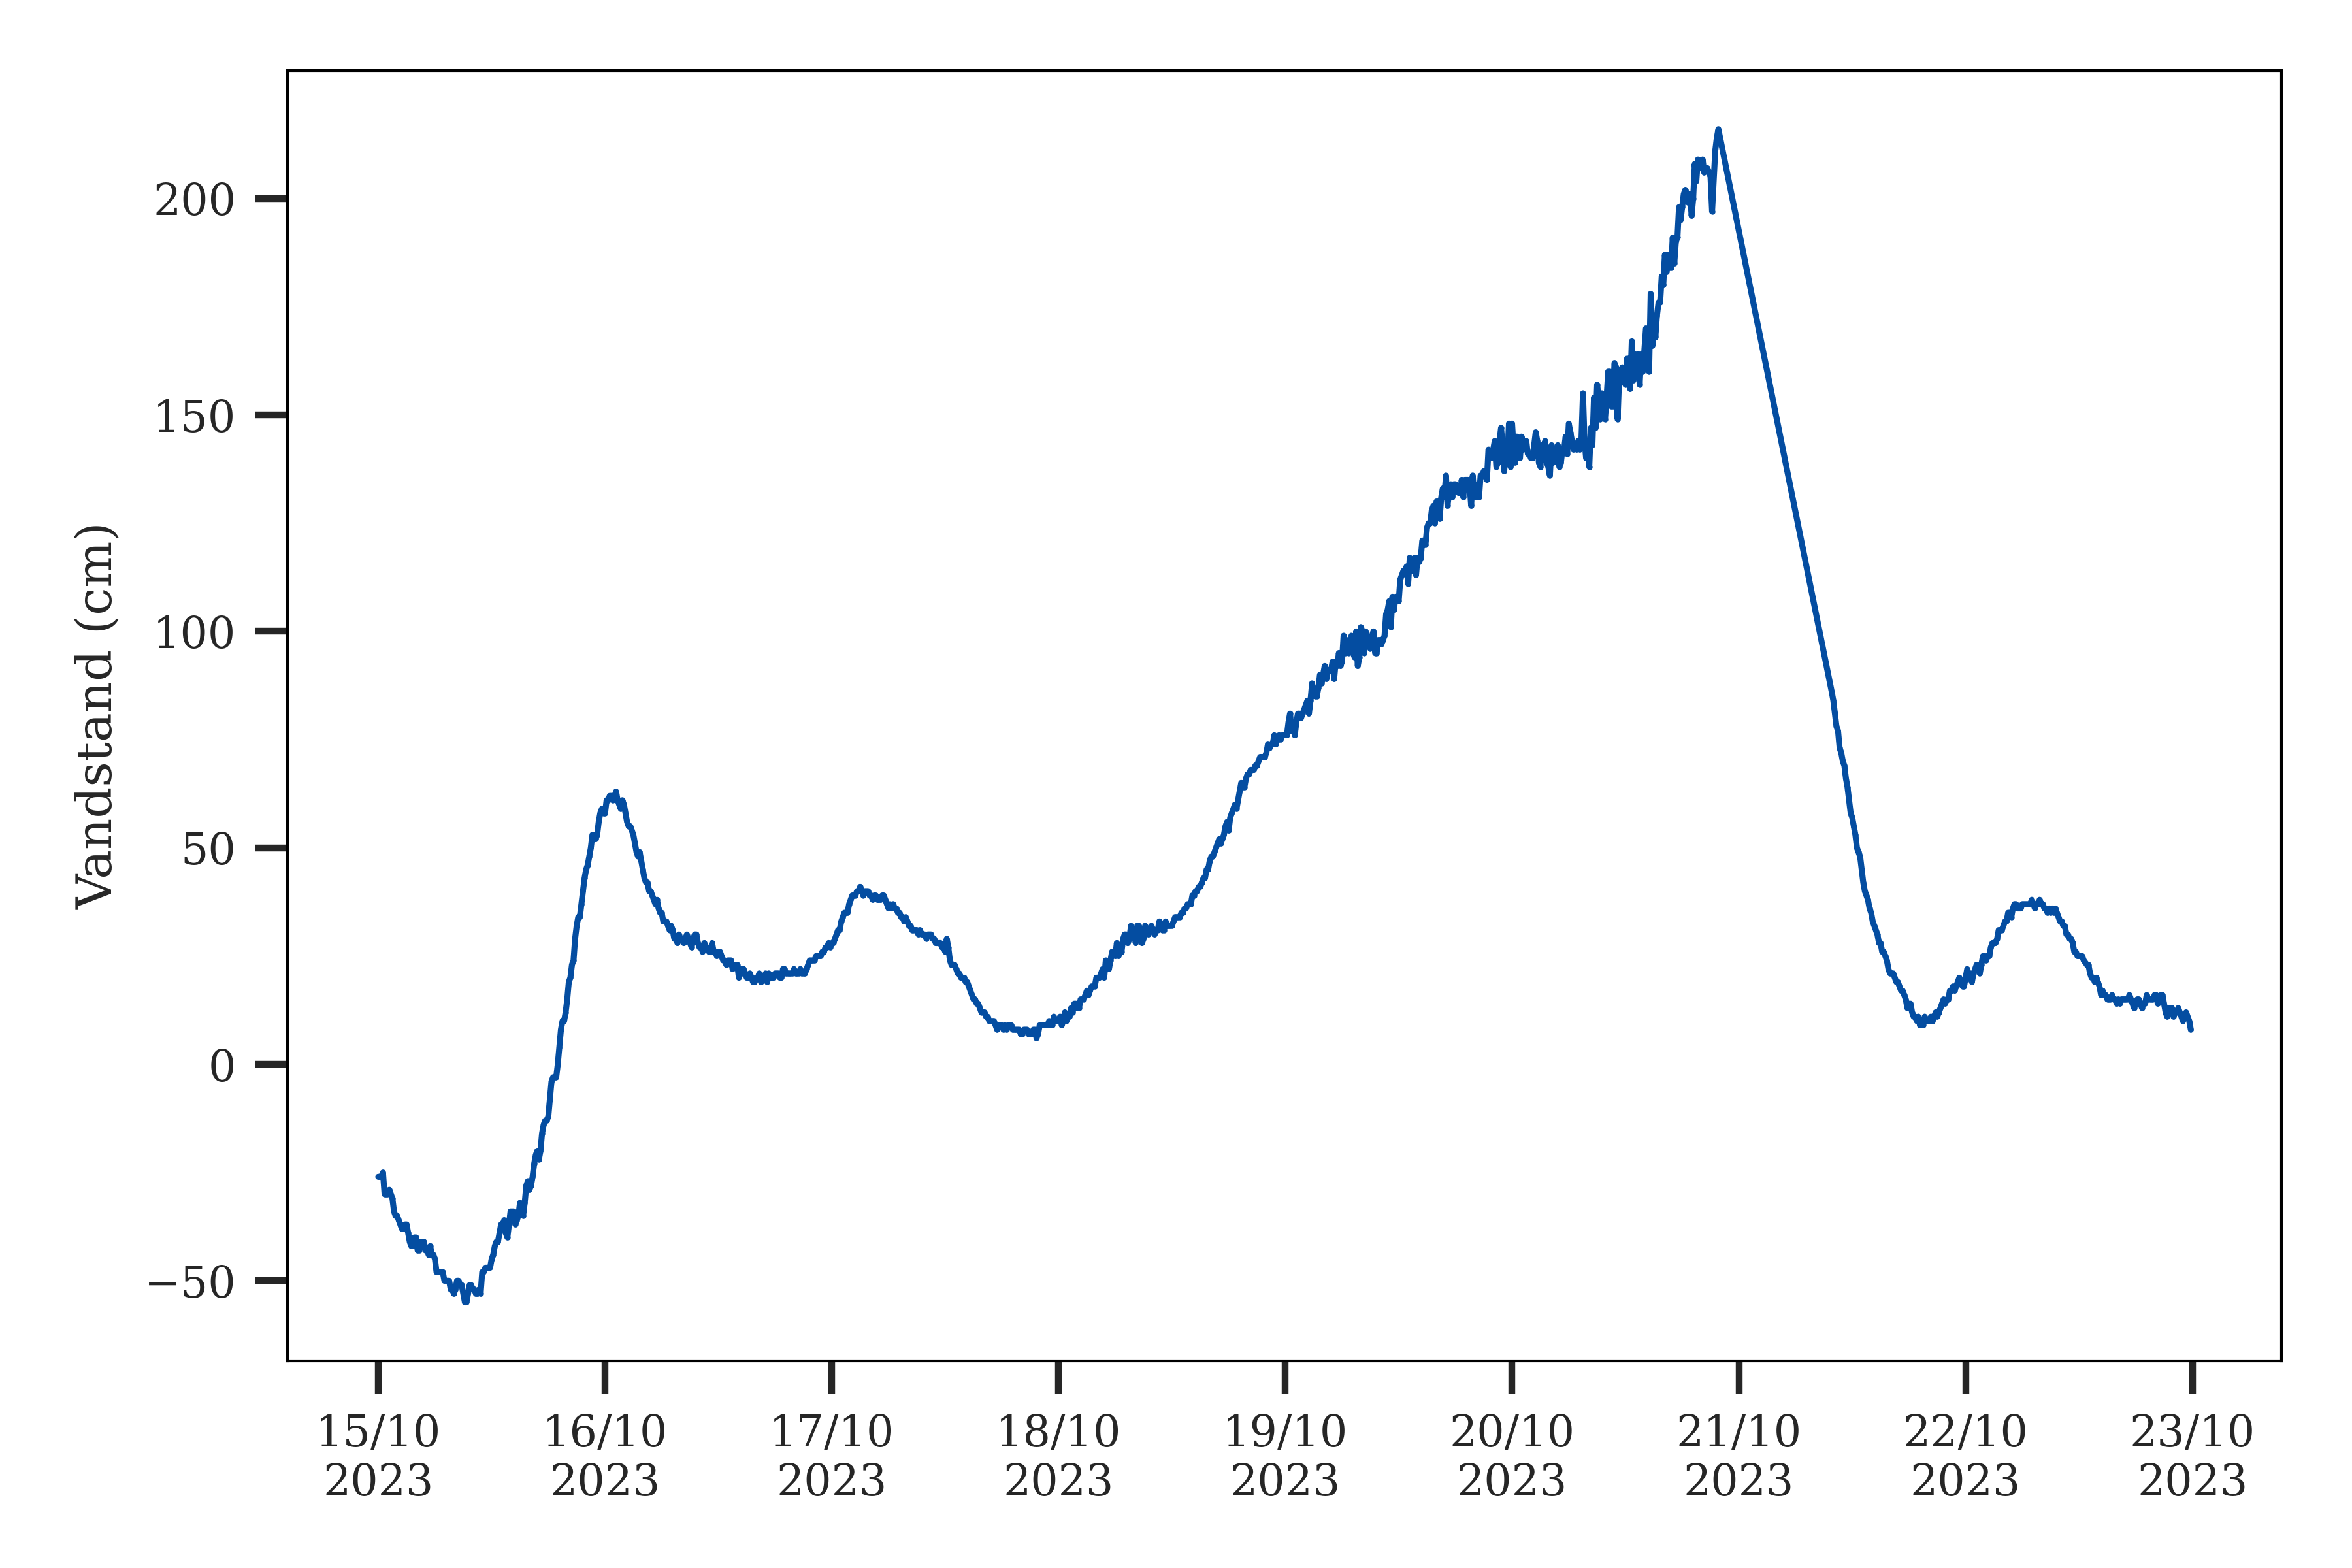
\includegraphics[width=1\textwidth]{images/vandstands_grafer/vandstand_aabenraa_vandstandsplot.png}
        \caption{Vandstanden i Aabenraa fra 15. til 23. oktober 2023.}
        \label{Subfig: Aabenraa vandstand}
    \end{subfigure}
    \hspace{0.2cm}
    \begin{subfigure}[b]{0.5\textwidth}
        \centering
        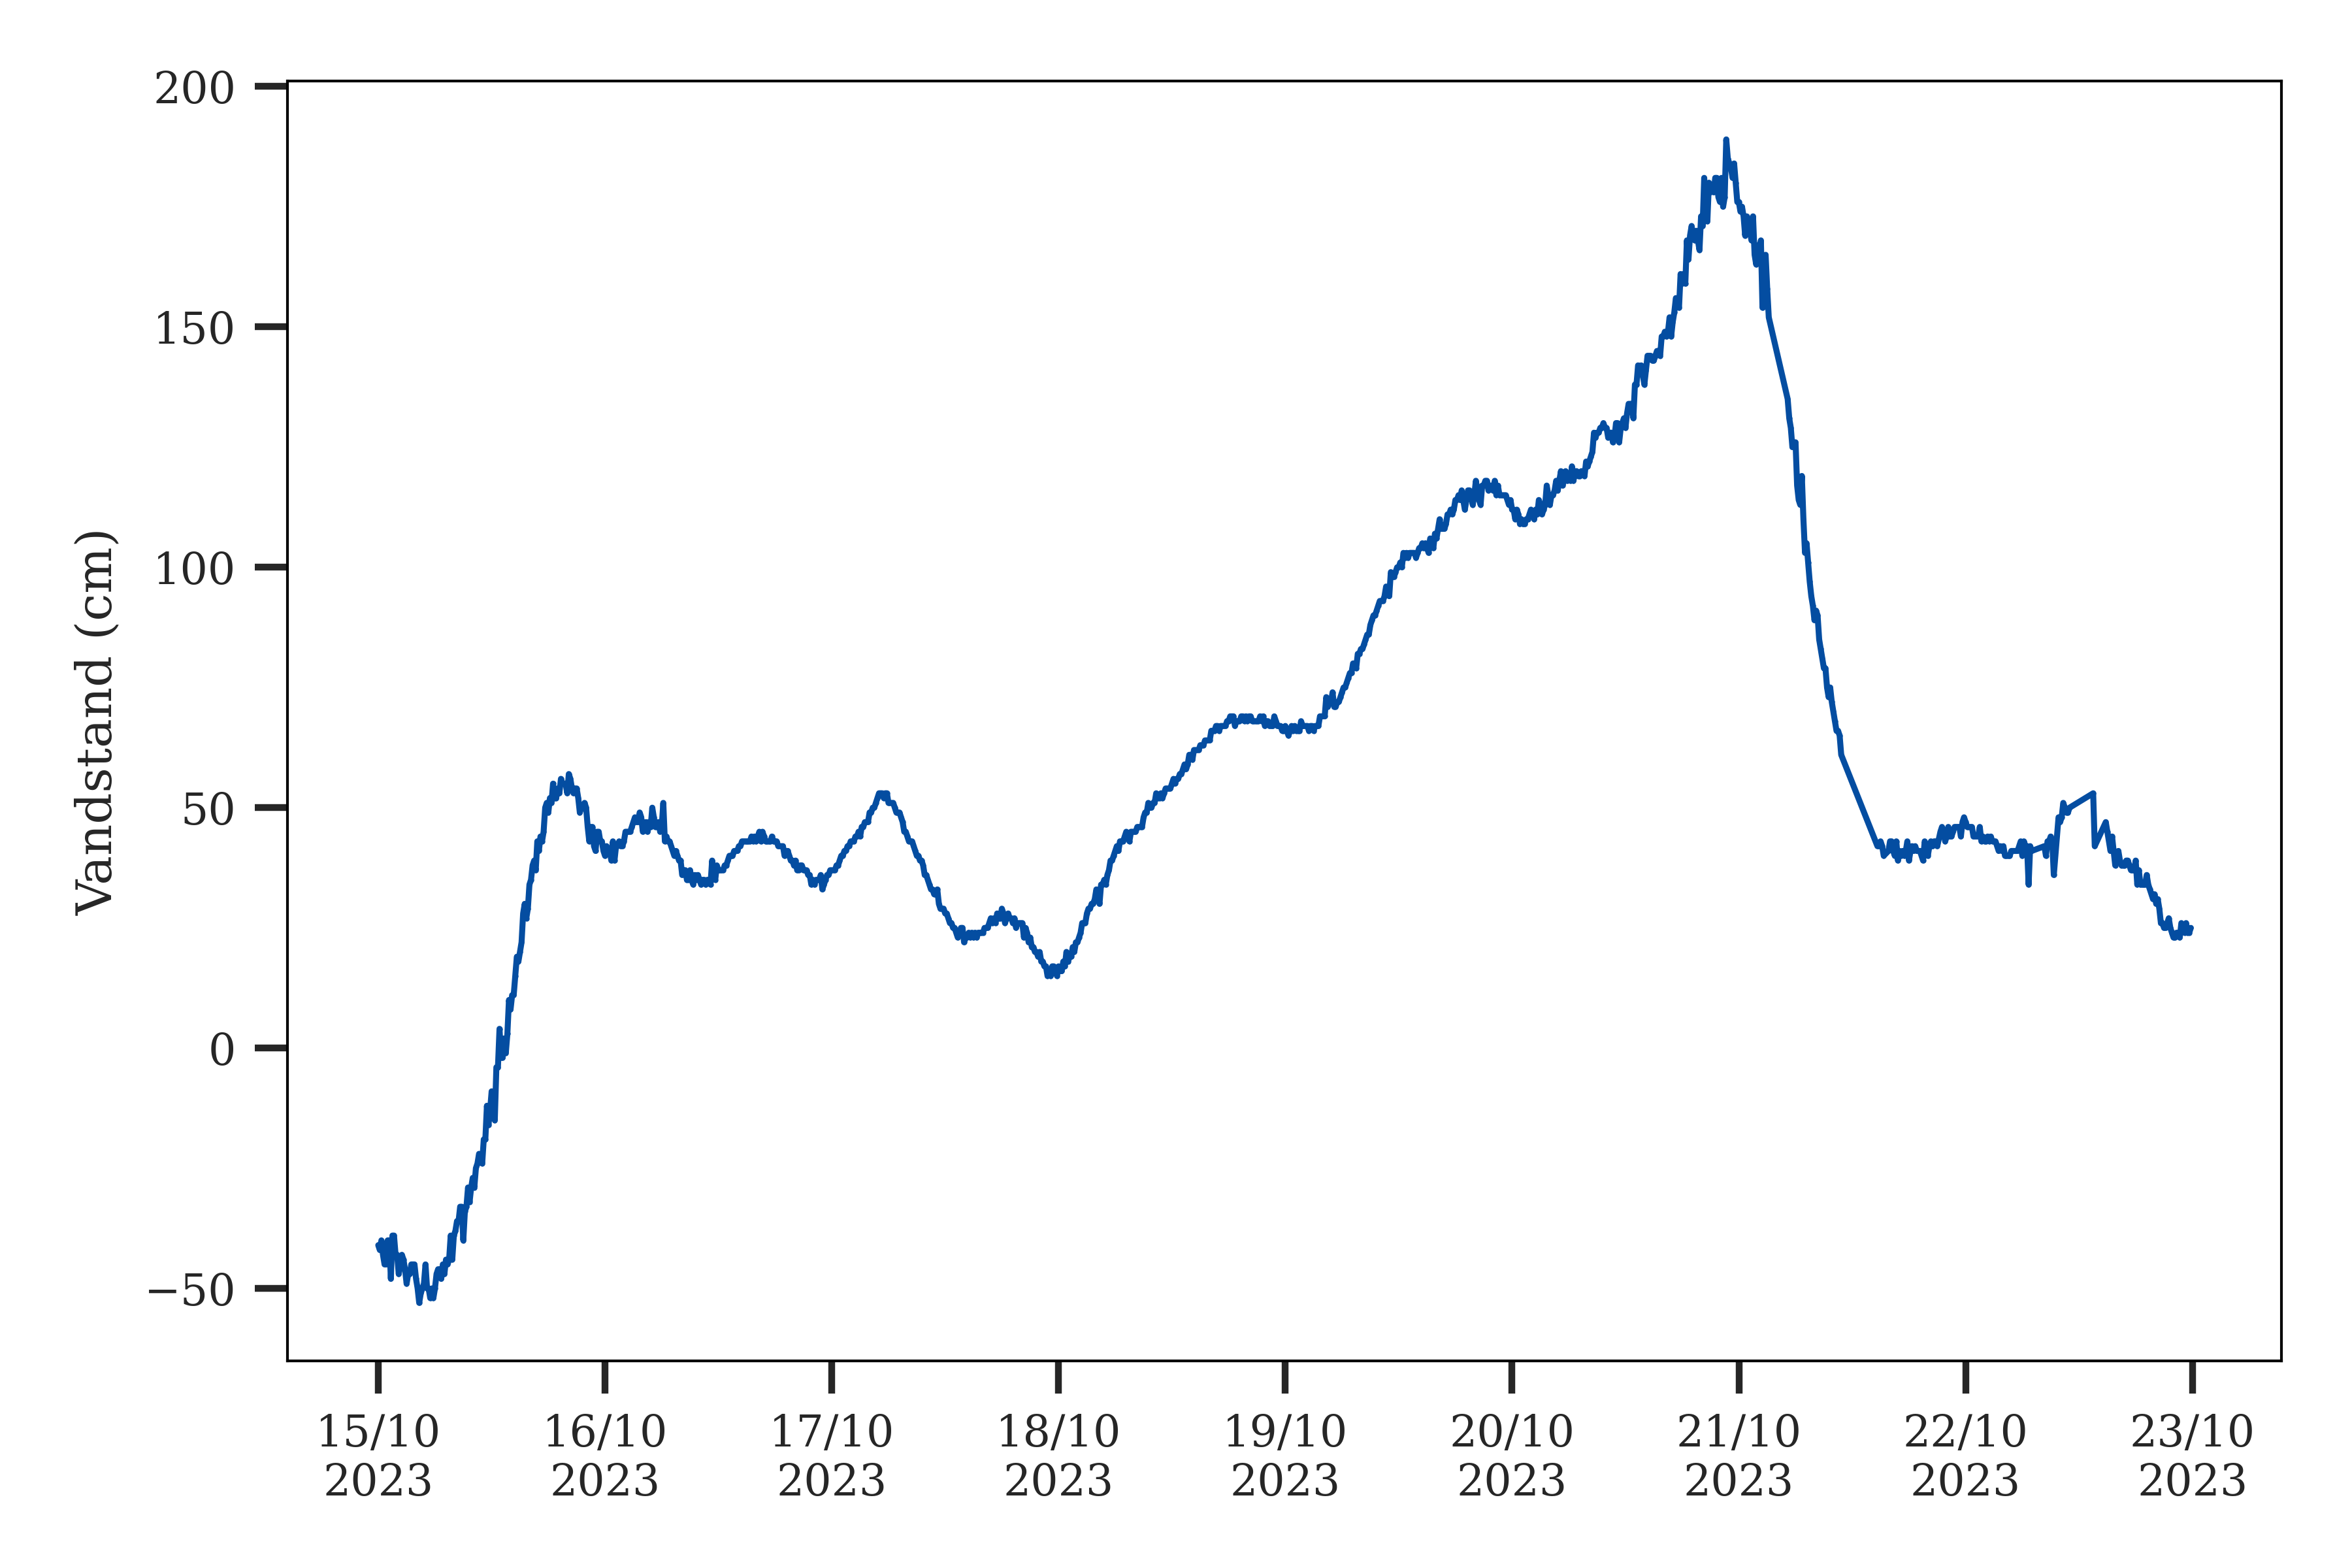
\includegraphics[width=1\textwidth]{images/vandstands_grafer/vandstand_gedser_vandstandsplot.png}
        \caption{Vandstanden i Gedser Havn fra 15. til 23. oktober 2023}
        \label{Subfig: Gedser vandstand}
    \end{subfigure}
    \vspace{0.2cm}
    \begin{subfigure}[b]{0.5\textwidth}
        \centering
        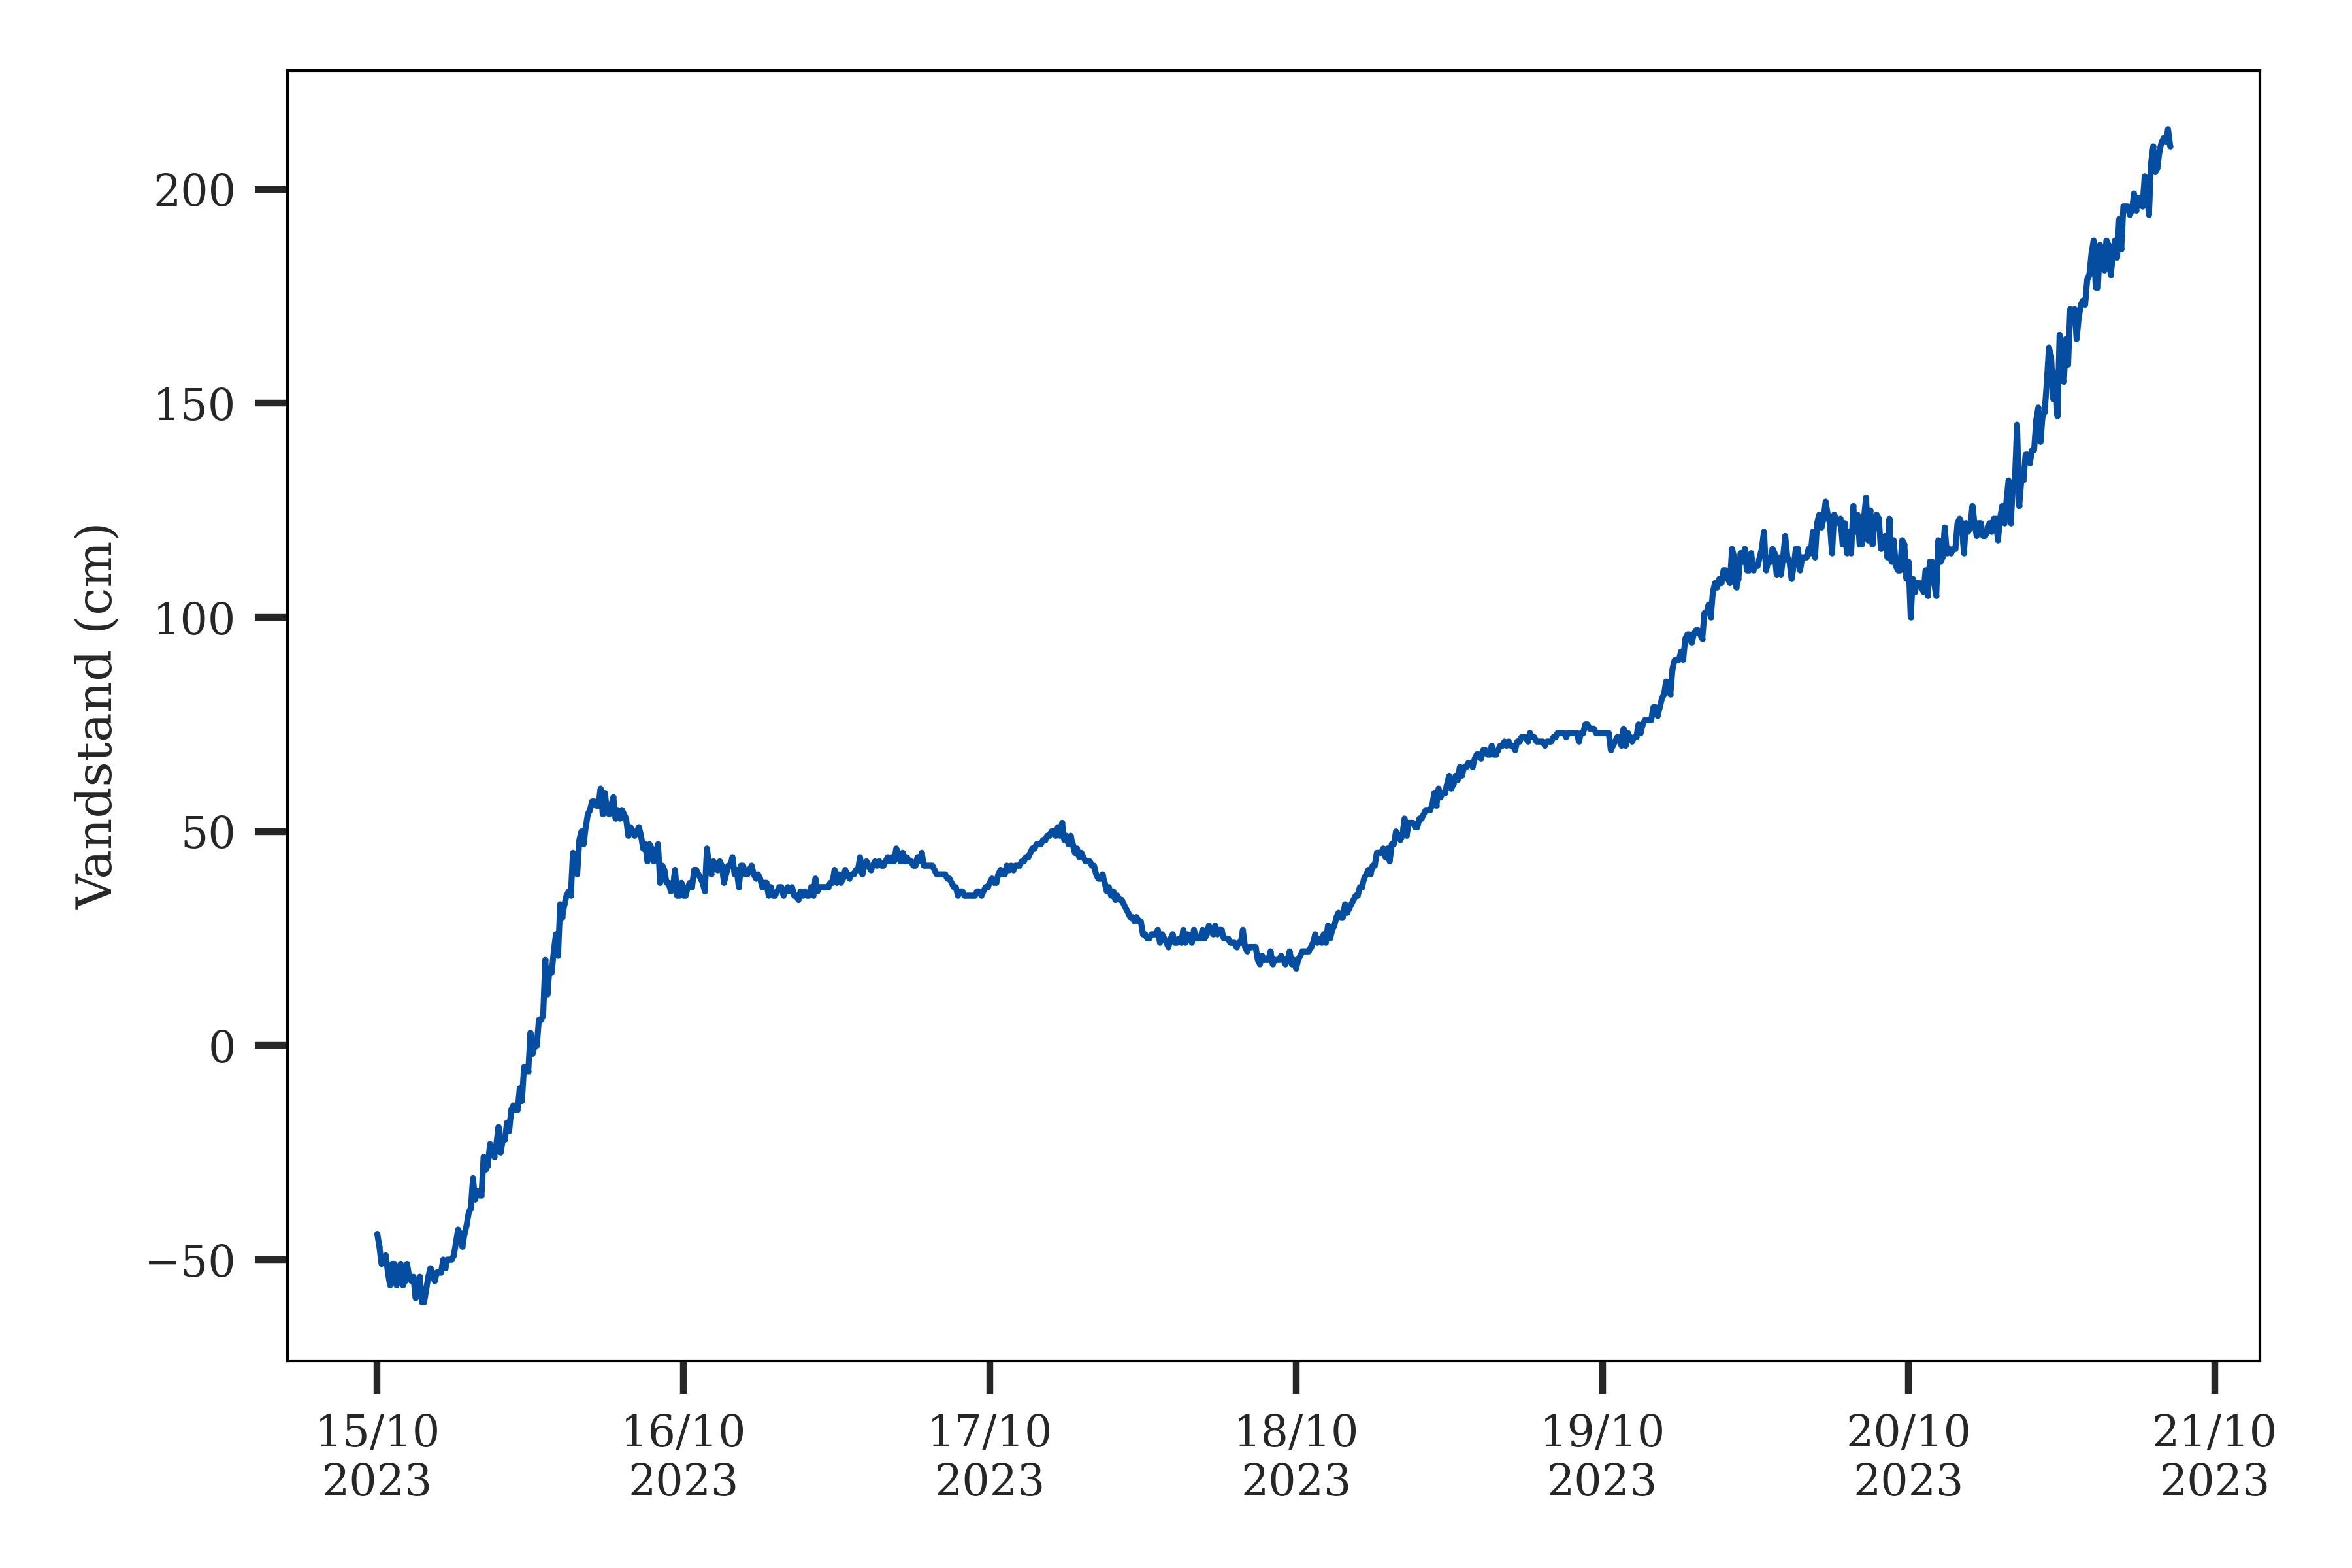
\includegraphics[width=1\textwidth]{images/vandstands_grafer/vandstand_hesnaes_vandstandsplot.png}
        \caption{Vandstanden i Hesnæs fra 15. til 21. oktober 2023}
        \label{Subfig: Hesnæs vandstand}
    \end{subfigure}
    \hspace{0.2cm}
    \begin{subfigure}[b]{0.5\textwidth}
        \centering
        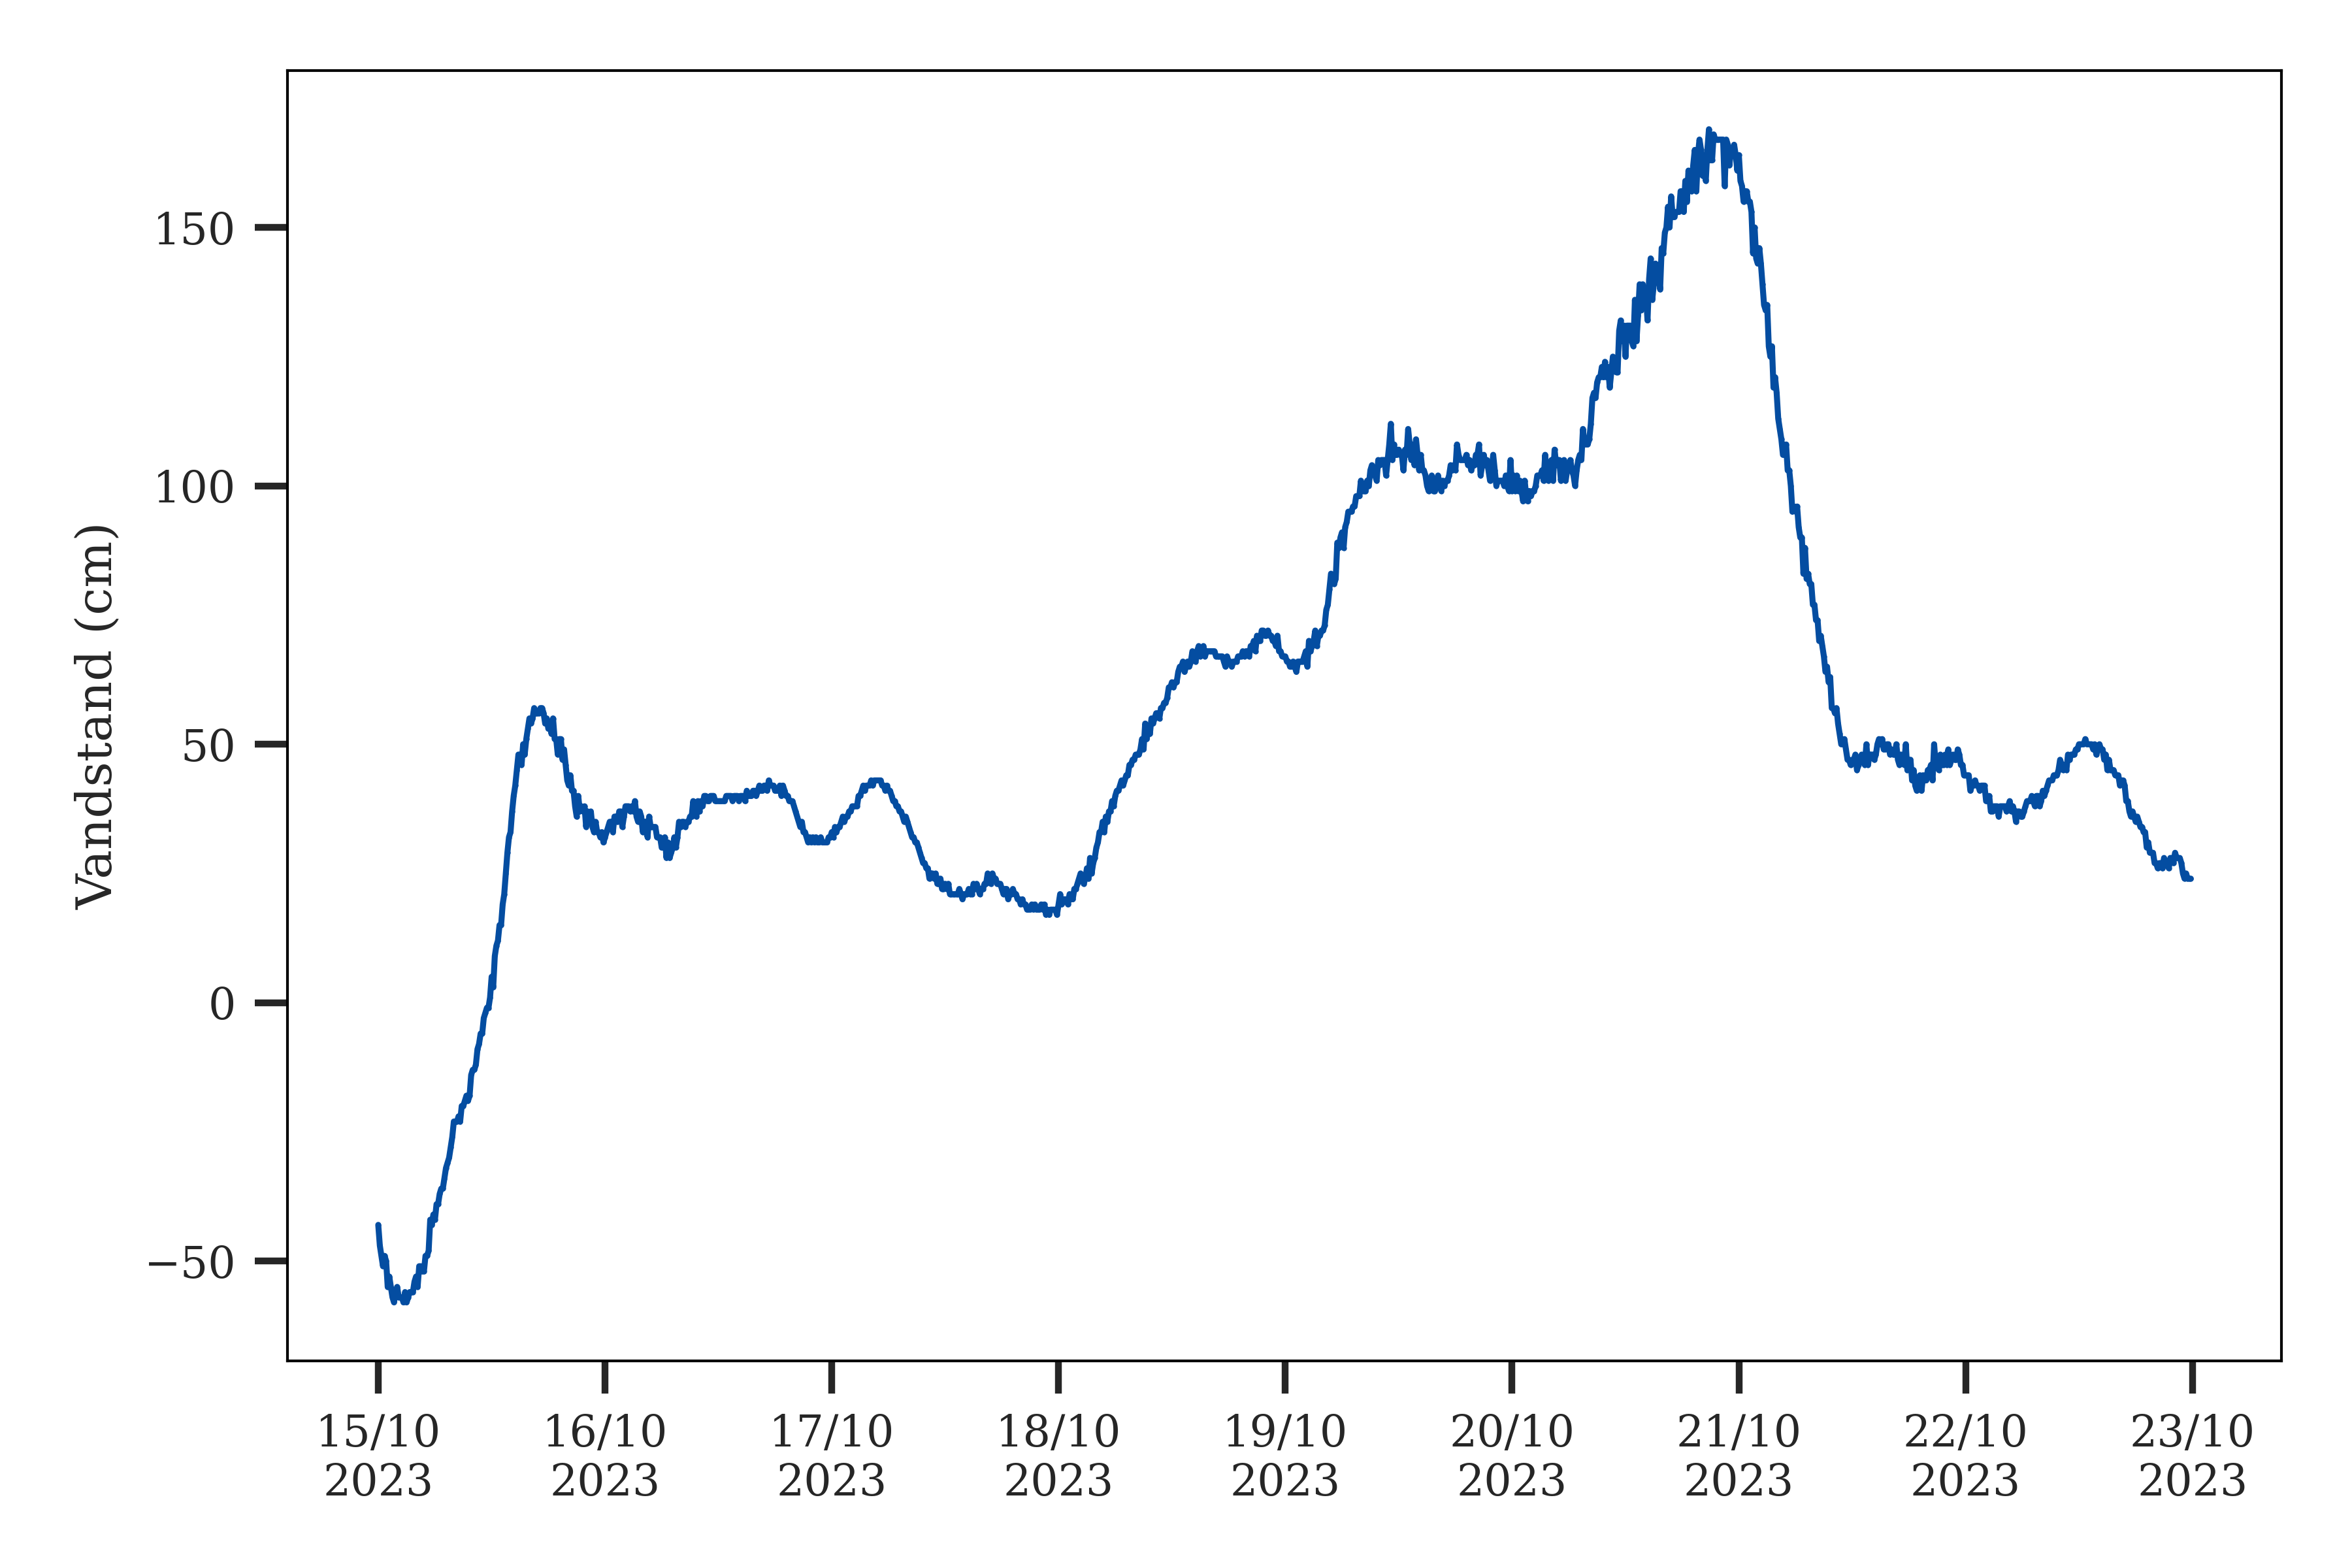
\includegraphics[width=1\textwidth]{images/vandstands_grafer/vandstand_praestoe_roedvig_vandstandsplot.png}
        \caption{Vandstanden i Rødvig fra 15. til 23. oktober 2023}
        \label{Subfig: Rødvig vandstand}
    \end{subfigure}
    \caption{Vandstanden i studieområderne Aabenraa, Gedser Havn, Hesnæs og Rødvig fra den 15. til 23. oktober. Kilde: Data stammer fra DMI og DMI Frie Data API-resource}
    \label{Figur: Vandstandsdata}
\end{figure}
Hesnæs er et lille fiskerleje og landsby på det østlige Falster i Guldborgsund kommune. Hesnæs fungerer som en havn og er den eneste på Falsters østkyst. Hesnæs er beliggende inde mellem to skove: Corselitze skov mod nord og Bønnet skov mod syd, som begge går helt ud til skrånede klinter ud til Østersøen. \\
Hesnæs blev særdeles hårdt ramt af stormfloden den 20 oktober 2023, hvor der blev officielt målt 2,10 m vandstand over DVR90. Uofficielle målinger nåede helt op på 2,39 meter over DVR90, men måleren gik i stykker kort tid efter (figur \ref{Subfig: Hesnæs vandstand}). Meget af Hesnæs havn blev svært beskadet af stormen, især den ydre mole af havnen blev ødelagt og lystbådhavnen blev dermed sat ud af drift på ubestemt tid. \\

Præstø er en havneby og en tidligere købstad i Vordingborg Kommune på Sjælland. Byen er beliggende i den sydlige del af Præstø Fjord, bag halvøen Feddet i bunden af Faxe Bugt. Tværs igennem byen løber tunneldalen Tubæk Å, et vandløb der deler byen mellem et nordligt handelscentrum og et sydligt boligkvarter. Byen har en befolkningstal på 3939 i 2025 \citep{danmarks_statistisk_mobile_nodate} og er kommunens anden største by. \\
Under stormfloden den 20 oktober 2023 blev store dele af Præstøs handelscentrum oversvømmet, især efter sluseporten der bruges til tilbageholde vandet i Tubæk Å, brød sammen \citep{uldall_sluseport_2023}. Der er ingen officielle målinger om vandstandshøjden i Præstø under stormfloden, da den nærmeste målestation er placeret længere opstrøms af Tubæk Å. \cite{cowi_praesto_2025} giver et skøn på at vandstanden var ca. 40 cm højere end i Rødvig Havn i Stevs Kommune ca. 25 km nordøst fra Præstø. Dette giver en vandstand på 2 meter over DVR90 under stormfloden i Præstø (figur \ref{Subfig: Rødvig vandstand}).



\section{Metoder}
% DE RIGTIGE SIDER!!!!
%\subsection{Databeskrivelse}

\subsection{Databehandling}
%\subsection{Inundation Model}

\subsubsection{Konverteringen fra DTM til DHyM}

\subsubsection{Inkludering af bygninger i DHyM}

\subsubsection{Create Inundation}



%Alt dette er udkast og SKAL SLETTES!!!!
Der vil i dette afsnit blive beskrevet den metodiske tilgang til projektets analyse og resultater. Der vil først blive beskrevet de dataprodukter der er anvendt og det databehandlinger der er blevet udført. Derefter beskrives arbejdstilgangen bag brugen af Inundation Modellen og hvordan den fremskrevne stormflod er beregnet. \\
Metodiske fravalg og fejlkilder vil blive diskuteret i sektion \ref{Resultat Diskussion} 

\subsection{Databeskrivelse og databehandling} \label{Sektion: Databeskrivelse}
% god teknik er at lave en label til sektionen, så den er nem at referere til (just in case).


I den følgende sektion vil der blive beskrevet det data der er blevet anvendt i projektet. Herudover vil der også blive beskrevet hvordan data eventuelt er blevet ændret i forhold til det originale data. 

\subsubsection{Digital Terræn Model} \label{Afsnit: Digital Terræn Model}
Modellering og simuleringer af oversvømmelser fra havet kræver en digital terræn model (DTM). En DTM er en digital repræsentation af højderne i landskabet i forhold til en reference og adskiller sig fra en Digital Overflademodel (DSM) ved ikke at inkludere bygninger og træer \citep{sdfe_dhm_2020}. En DTM bliver dannet ved brug af LiDAR flyscanning og optages i Danmark over en 5-årig periode i forskellige sektioner. 
I Danmark er det Klimadatastyrelsen (\textit{tidl.} Styrelsen for Digitalisering og Infrastruktur), som står for etableringen af DTM for hele landet \citep{sdfe_dhm_2020}. \\

I dette projekt er der anvendt den seneste opdateret DTM fra 2023. For Aabenraa, Gedser og Hesnæs er DTM blevet optaget i 2023, mens DTM for Præstø er seneste optaget i 2019. DTM for Danmark lagres i et GeoTIFF rasterformat med en cellestørrelse på 0,4$\times$0,4m (0,16 m\textsuperscript{2}). DTM'en er i en UTM zone 32N projektion og i ETRS89 koordinatsystemet med en horisontal nøjagtighed på \pm 1 m. Den vertikale reference er i DVR90 med en vertikal nøjagtighed på \pm 5 cm \citep{sdfe_dhm_2020}. \\
DTM'en anvendt i dette projekt er blevet ændret baseret på størrelsen af hvert studieområde. DTM blev skåret ned til en brugerdefineret afgrænsning af hvert studieområde for at minimere processeringstid. Afgræsningen skete på baggrund af studieområdets topografi og udstrækket af eventuel byzone. Derudover er DTM blevet konverteret til en Digital Hydrologisk Model (DHyM) og bygningspolygoner er blevet brændt ned som ikke passerbare enheder i terrænet. Fremgangsmåden for dette er beskrevet i sektion \ref{Sektion: Konvertering af DTM til DHyM} og \ref{Afsnit: Inklusion af bygninger i DHyM}.  


\subsubsection{Arealanvendelses data} \label{Afsnit: Arealanvendelses data}
For at undersøge og kvantificere oktober 2023 stormflodens påvirkning af de udvalgte studieområder, anvendes der et arealanvendelses datasæt til at beregne og identificere de påvirkede arealanvendelser under stormfloden. \\
Dette blev gjort ved at bruge det danske arealanvendelses datasæt BaseMap produceret af \cite{Jepsen_levin_2013}. BaseMap dækker omtrent 98\% af Danmarks areal med 35 forskellige arealanvendelsesklasser og er leveret i et rasterformat med en cellestørrelse på 10\times10 m. Kortet er seneset opdateret i 2022 med version fire og det er denne version der er anvendt \citep{levin_basemap04_2022}.\\

For at forsimple visualiseringen af påvirkede arealanvendelser er der blevet udført en reklassifikation af arealklasserne på samme måde som \cite{balstrom_kirby_inundation}. Med denne reklassfikation blev arealanvendelses datasættet trimmet fra 35 oprindelige arealklasser til 13 overordnede klasser. Ved reklassificeringen er en række af klasserne herunder lufthavn, råstofudvinding og Tyskland, som ikke er tilstede i studieområderne, blevet ekskluderet. Klasserne hav, vandløb og søer er også blevet ekskluderet, da de ikke har en relevans for undersøgelsen.\\ 
Dette resulterer i 8 overordnede klasser der er vist i tabel \ref{Tabel: arealanvendelses klasser} samt hvilke klasser fra BaseMap der indgår i de nye aggregerede arealklasser.
\begin{table}[H]
\centering
\renewcommand{\arraystretch}{1.5}
\begin{threeparttable}
\caption{Reklassificerede arealklasser baseret på \cite{balstrom_kirby_inundation} og hvilke arealklasser fra Basemap \citep{Jepsen_levin_2013} der indgår i hver klasse.}
\label{Tabel: arealanvendelses klasser}
\begin{tabular}{@{} l l l @{}} 
\toprule
\textbf{ID} & \textbf{Aggregerede klasser} & \textbf{BaseMap04 klasser} \\
\midrule
1 & Bebyggede områder &
  \makecell[l]{Bygning, Lav bebyggelse, Lav bebyggelse; Bygning,\\
  Høj bebyggelse, Høj bebyggelse; Bygning,\\
  Bykerne, Bykerne; bygning, Andet bebyggelse,\\
  Andet bebyggelse; Bygning} \\ 
  \addlinespace
2 & Erhverv &
  \makecell[l]{Erhverv, Erhverv; Bygning} \\
  \addlinespace
3 & Rekreativt &
  \makecell[l]{Rekreativt område / sportsanlæg,\\
  Rekreativt område / sportsanlæg; Bygning} \\
  \addlinespace
4 & Infrastruktur &
  \makecell[l]{Vej; befæstet, Vej; ikke befæstet,\\
  Jernbane, Jernbane; Bygning} \\
  \addlinespace
5 & Landbrug &
  \makecell[l]{Landbrug intensivt; midlertidige afgrøder,\\
  Landbrug intensivt; permanente afgrøder,\\
  Landbrug ekstensivt, Landbrug; ikke klassificeret} \\
  \addlinespace
6 & Skov &
  \makecell[l]{Skov, Skov; Våd} \\
  \addlinespace
7 & Naturområde &
  \makecell[l]{Natur; tør, Natur tør; Landbrug ekstensivt,\\
  Natur; våd, Natur våd; Landbrug ekstensivt} \\
  \addlinespace
8 & Uklassificeret &
  \makecell[l]{Ikke kortlagt} \\
\bottomrule
\end{tabular}
\end{threeparttable}
\end{table}


\subsubsection{Hydrologiske tilpasninger} \label{Afsnit: Hydrologiske tilpasninger}
I processen for at konvertere en DTM til DHyM er der blevet anvendt to hydrologiske tilpasningslag: Linje- og hesteskotilpasninger. Tilpasningerne er begge geometriske et-dimensionelle dataobjekter defineret af GeoDanmark som linjer \citep{GeoDanmark_HydroLag}. \\
Linjetilpasningerne er en defineret som et linjeobjekt, der beskriver en åbning for overfladevands forløb gennem en hindring eller en hindring af overfladevands forløb gennem et terræn \citep{DHMLinje}. 
Linjetilpasningerne er den simpleste hydrologiske tilpasning og forekommer ved bl.a. rør og små vandløb der passerer under veje eller mellem marker. I figur \ref{Subfig: Linjetilpasning} er det et eksempel på en linjetilpasning gennem et rør fra en mark.\\

Hesteskotilpasningerne er defineret af \cite{DHM_Hestesko}, som et hestesko-formet geometrisk objekt der tillader eller begrænser overfladevandets forløb gennem en hindring eller gennem terrænet. Bredden af hesteskoen definerer dermed hindringens størrelse. Hesteskotilpasningerne anvendes ved hindringer i landskabet der er større end et mindre vandløb eller rør og dermed kræver en mere korrekt repræsentation i landskabet. Hesteskotilpasningerne findes især under større broer og tunneller under veje og i figur \ref{Subfig: Hesteskotilpasning} er der vist et eksempel på en hesteskotilpasning fra en cykeltunnel under en vej.
\begin{figure}[H]
    \begin{subfigure}[b]{0.5\textwidth}
        \centering
        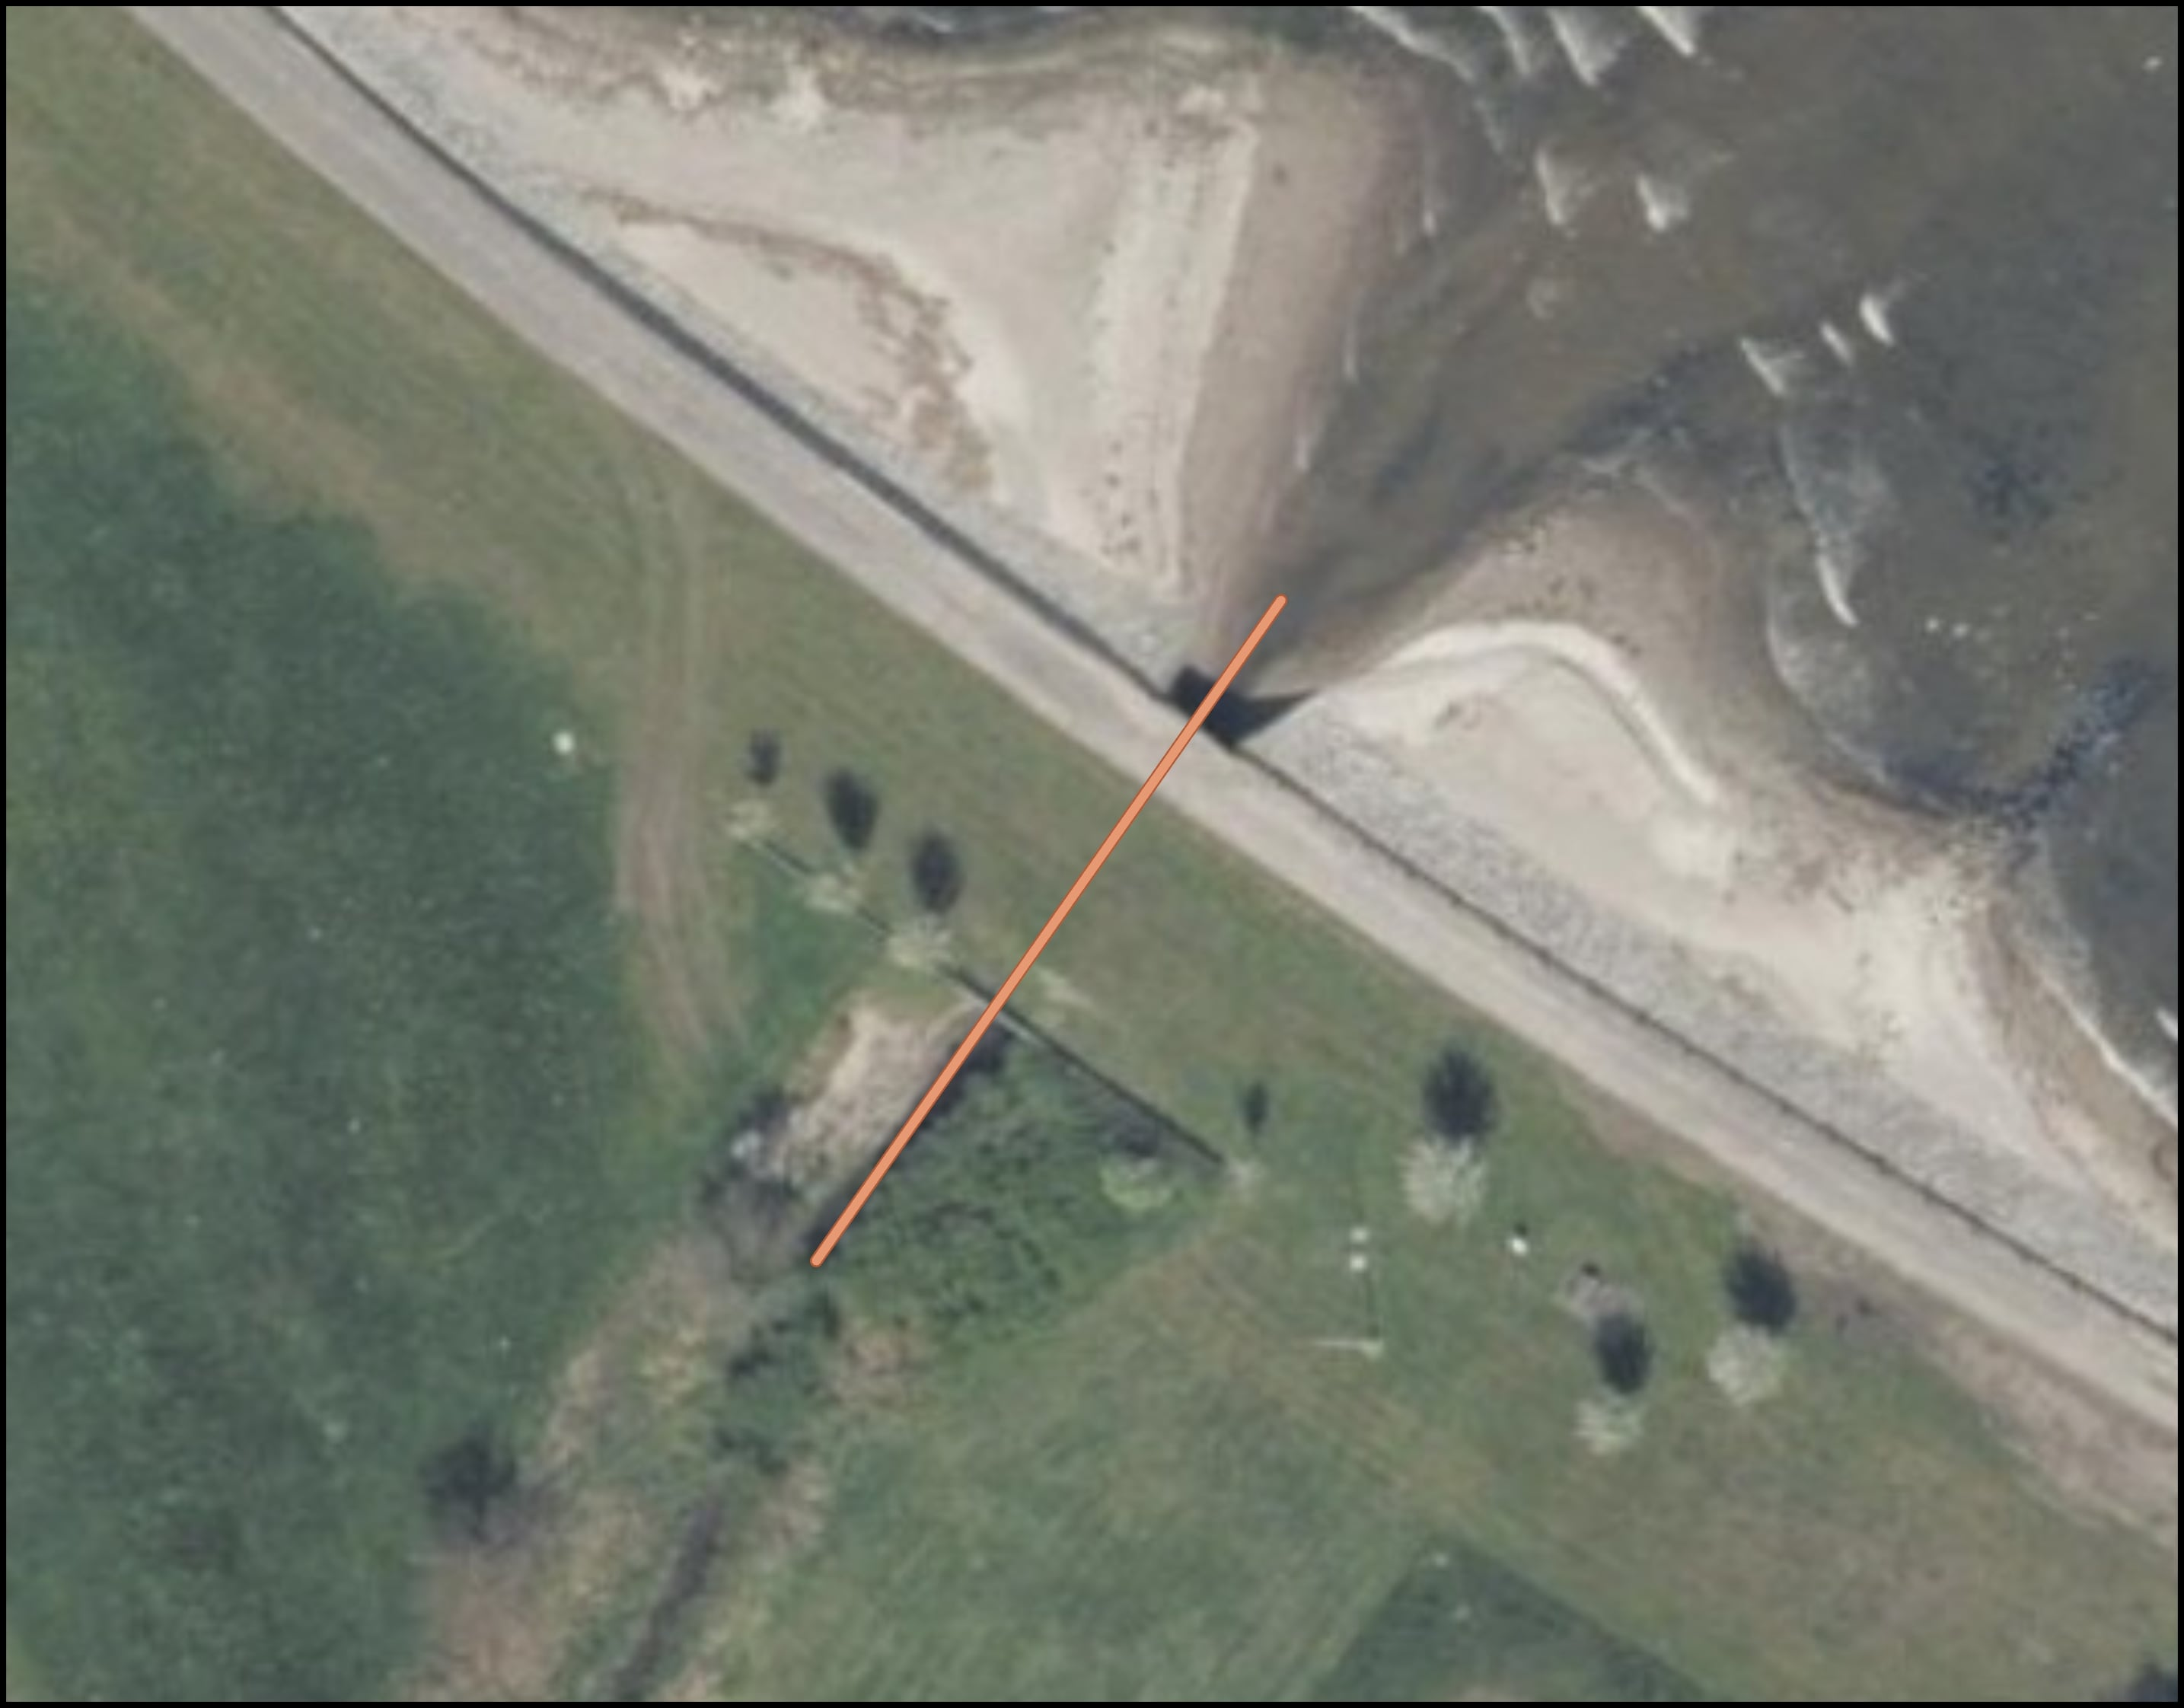
\includegraphics[width=1\linewidth]{images/databeskrivelse/linje.jpg}
        \caption{}
        \label{Subfig: Linjetilpasning}
    \end{subfigure}
    \hspace{0.2cm}
    \begin{subfigure}[b]{0.5\textwidth}
        \centering
        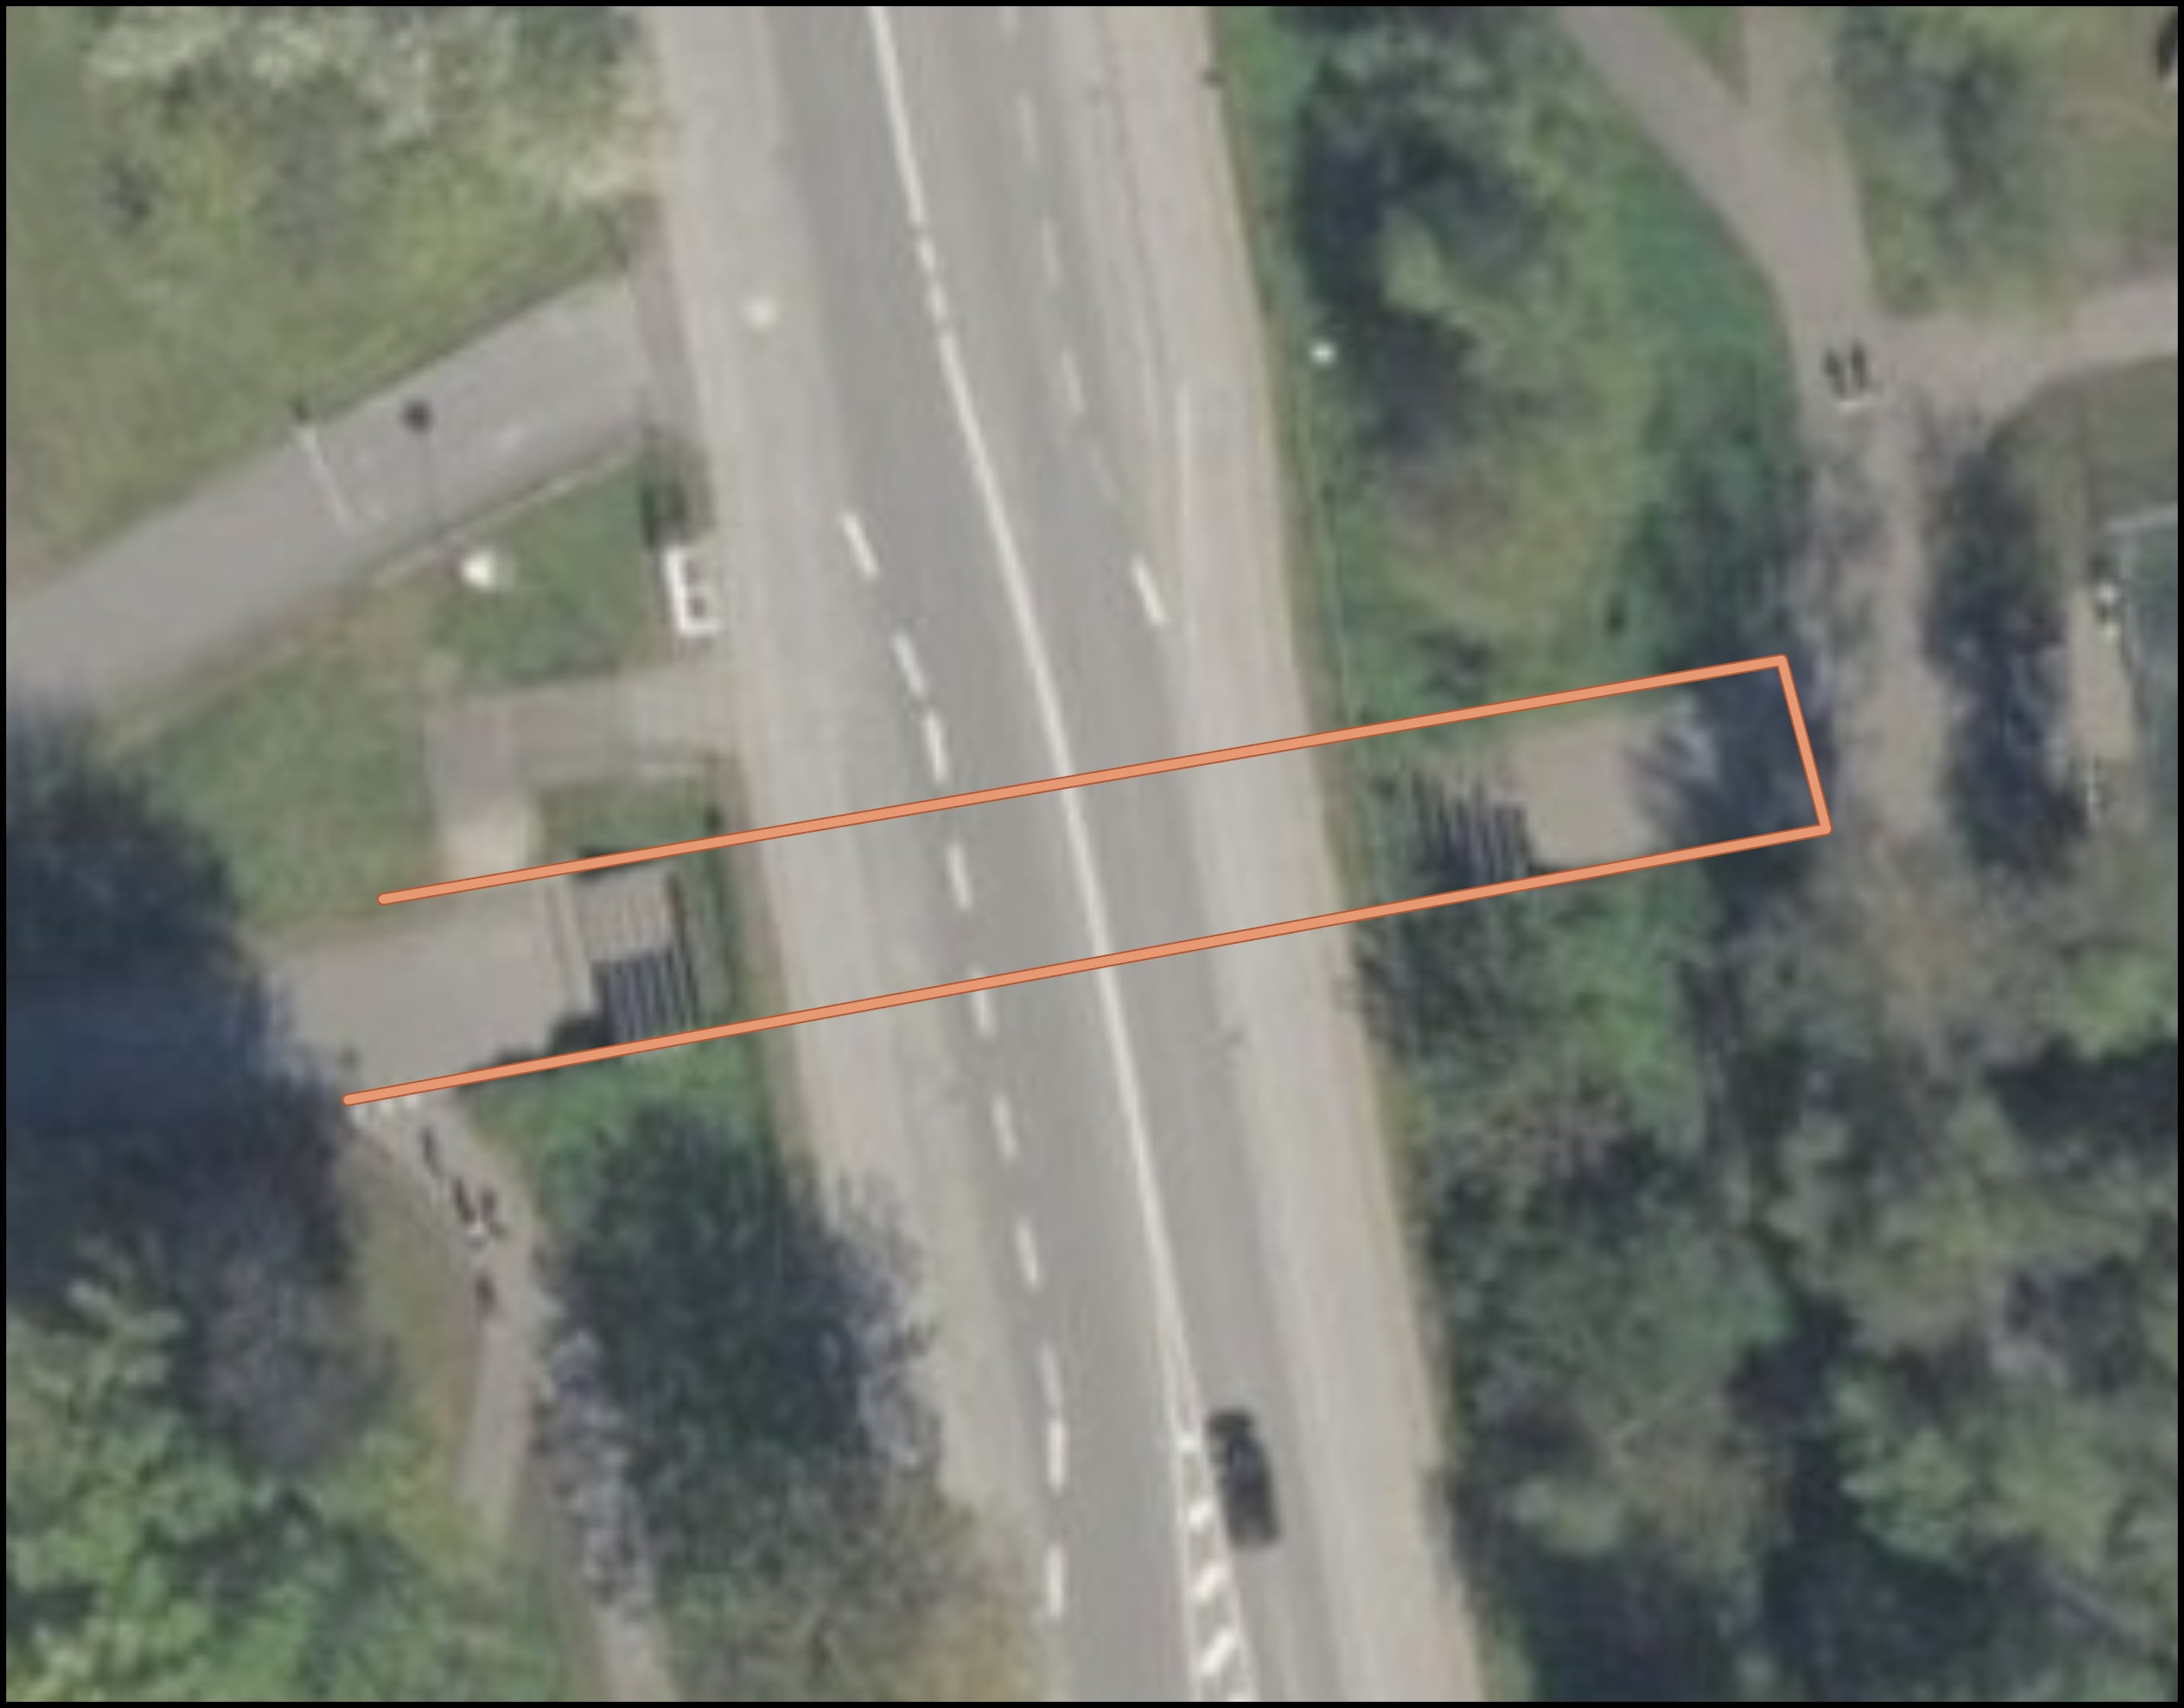
\includegraphics[width=1\linewidth]{images/databeskrivelse/hestesko.jpg}
        \caption{}
        \label{Subfig: Hesteskotilpasning}
    \end{subfigure}
    \caption{Eksempler på en \textbf{(a)} Linjetilpasning fra et mindre vandløb under en græsplæne. \textbf{(b)} Hesteskotilpasning fra en cykeltunnel under en vej i Aabenraa. }
    \label{Figur: Linje- og hesteskotilpasninger}
\end{figure}


\subsubsection{Vind- og vandstandsdata} \label{Vind- og vandstandsdata}
Til at forstå konteksten bag stormflods hændelsen den 20-21. oktober 2023 er der blevet anvendt vind-og vandstandsdata for måneden oktober 2023. \\
Vinddata er indsamlet fra Danmarks Meteorologiske Instituts (DMI) vejrarkiv \citep{dmi_vejrarkiv} for hele landet. 
Vinddata er beregnet som gennemsnit for middelvind, højeste 10-min middelvind og den maksimale vindhastighed i m/s for hver dag i måneden. \\

Vandstandsdata er indsamlet på to måder. Data fra Gedser, Hesnæs og Præstø er indsamlet direkte fra DMI's Open Data API-Oceanographic Observation Data ressource \citep{dmi_open_data}. Alt vandstandsdata er optaget hvert 10. minut fra den 1. oktober til den 31. oktober 2023 og er herefter filtreret til kun at vise data fra den 15. til den 23. oktober. Data for Præstø er hentet fra Rødvig Havn, ca 25,5 km nordøst, da Præstø ikke har en officiel DMI vandstandsmåler. Dette er den samme station, som \cite{cowi_praesto_2025} har anvendt. \\
Vandstandsdata fra Aabenraa Havn er givet direkte fra en samtale med DMI med tilladelse fra virksomheden Aabenraa Havn, da DMI ikke stiller havnens vandstandsmålinger til rådighed for offentligheden. \\

Vandstandsdata fra Gedser Havn havde en del afvigelser, hvor vandstanden svingede fra +200 cm til -340 cm på 10-min. De datapunkter er fjernet efter et kriterie om at vandstanden ikke vil ændre sig med mere end \pm 25\% på 10 minutter. Hvis vandstanden ikke er indenfor de grænsekriterier, så fjernes datapunktet og det efterfølgende datapunkt tages i betragtning. Hvis det næste datapunkt er indenfor grænsen, så bliver det datapunkt den nye værdi der tjekkes. Filtrerings logikken er vist i ligning \ref{Eq: Outlier vandstand}. Hvor $x$ er et datapunkt i serien og $x_i$ er det næste datapunkt i serien.
\begin{align} \label{Eq: Outlier vandstand}
    \text{Hvis } x_i \in [0.75\times x, 1.25\times x], \text{ så } x \leftarrow x_i \nonumber \\
    \text{Hvis } x_i \notin [0.75\times x, 1.25\times x], \text{ så fjernes } x_i
\end{align}

\subsubsection{Data fra studieområderne og andet anvendt data} \label{Afsnit: Data fra studieområderne og andet anvendt data}
Projektet benytter sig af data modtaget fra de tre kommunerne hvor undersøgelsen finder sted. Den primære dataform er et raster kort over vandets udbredelse fra stormflodshændelsen i 2023. Alle kortene blev resamplet til en cellestørrelse på 0,4\times0,4 m, for at sikre samme cellestørrelse som Inundation modellens resultat, da alle kortene havde forskellige cellestørrelser der variede mellem 0,45 og 0,5 m.\\
Aabenraa kommune har derudover givet information, linje- og punktdata omkring beredskabsindsatser, herunder placeringerne af watertubes og dronebilleder over byen.\\ 

Udover det ovennævnte data er der blevet anvendt en række mindre dataprodukter. 
Dette inkluderer et datasæt med bygningspolygoner der er blevet anvendt til at brænde bygninger ned i DHyM. I sektion \ref{Afsnit: Inklusion af bygninger i DHyM} er der beskrevet hvordan bygningspolygon datasættet er blevet ændret. En topografisk landpolygon over Danmark fra Klimadatastyrelsen, er anvendt som en afgrænsningsmaske til Inundation Modellens resultat. Et datasæt over vandstandsstignings projektioner for 2030 fra den sjette \cite{ipcc_report_AR6, garner_ipcc_2021} klimarapport samt et værktøj med stationsnumre for projektionerne fra \cite{NASA_tool}. Dette datasæt anvendes til at beregne udbredelsen af en fremskrevet stormflod vil se ud i slutningen af det nuværende århundrede.



\subsection{Konvertering af DTM til DHyM} \label{Sektion: Konvertering af DTM til DHyM}
Et vigtigt element af en realistisk oversvømmelsesmodellering er at kunne simulere korrekt hydrologisk adfærd gennem terrænet. Dette er essentielt for at kunne bruge modellens resultater tillidsfuldt at den digitale terrænmodel (DTM) bliver korrigeret og konverteret til en digital hydrologisk model (DHyM).\\ 

For at konvertere en DTM til DHyM bliver der anvendt to hydrologiske tilpasningsobjekter: Linje- og hesteskotilpasninger. Begge objekter er linjeobjekter og bliver brændt ned i DTM for at simulere korrekt geografiske karakteristika i landskabet, som ikke er blevet fanget af højdemodellen. \\
Da der findes tilpasninger for både simuleringer af skybrud og stormfloder, er det vigtigt at der kun bliver anvendt de tilpasninger der har indflydelse på havstigning- og stormflodsmodellering. Det betyder derfor at der ikke skal inkluderes tilpasninger, som er designet til at føre regnvand fra skybrud ud i havet. Tilpasninger såsom skybrudskontraklappe er derfor blevet fravalgt ved at udføre en selektering af de korrekte tilpasninger i databasen for hvert område.\\

Dette er gjort for både linje- og hesteskotilpasningerne ved brug af værktøjet \textit{"Extract Hydroconditoning Inundation"}, som foretager en søgning i databaserne for tilpasningslagene. Først søger værktøjet efter alle tilpasninger indenfor studieområdet defineret ud fra studieområdernes afgrænsning. Herefter laves der en søgning i attributtabellen for en anvendelses beskrivelse. Til stormflodsmodellering skal der anvendes tre attributter og deres funktionalitet er beskrevet i tabel \ref{Tabel: Relevante hydrologiske tilpasninger}. De tilpasninger som opfylder én af kriterierne bliver overført til et nyt lag, en for linjetilpasninger og en for hesteskotilpasninger. 
\begin{table}[H]
\centering
\renewcommand{\arraystretch}{1.5}
\begin{threeparttable}
\caption{Relevante hydrologiske tilpasninger for stormflodsmodellering. Kilde: \cite{GeoDanmark_HydroLag}}
\label{Tabel: Relevante hydrologiske tilpasninger}
\begin{tabular}{@{} l l @{}} 
\toprule
\textbf{Tilpasningstype} & \textbf{Beskrivelse af tilpasningen} \\
\midrule
\textit{Generel} &
  \makecell[l]{Den normale tilpasning af hydrologiske forhold\\
  (fx skabelse af et frit forløb under en bro)} \\
\addlinespace
\textit{Havstigning} &
  \makecell[l]{Tilpasninger der skal forhindre, at vand løber ind\\
  over det bagvedliggende land\\
  (fx lukning af en højvandssluse)} \\
\addlinespace
\textit{DHMFix} &
  \makecell[l]{Bruges ved ændringer, der har hydrologisk effekt\\
  på vandets frie forløb på terrænoverfladen\\
  (fx reparation af fejl i den specifikke DHM)} \\
\bottomrule
\end{tabular}
\end{threeparttable}
\end{table}

Inden tilpasningerne blev brændt ned i DTM, ændres hesteskotilpasningerne fra deres hesteskoform til at have en række linje mellem ydrekanterne af hesteskoen. Dette gøres for at få den præcise størrelse og udbredelse af tilpasningen brændt ned i DTM fremfor for omridset af tilpasningen. Det er blevet gjort ved at bruge et Python-script \textit{"Convert Horsehoes to Lines"} hvor både linje- og hesteskotilpasningerne fundet i \textit{"Extract Hydroconditioning Inundation"} bliver omdannet til separate linjer. Konverteringen til separate linjer gør beregningen af højdeværdier i tilpasingen nemmere og dermed nemmere at brænde ned i DTM.\\
De separate linjer til hesteskotilpasningerne blev defineret ud fra de 4 hjørnepunkter af hesteskoen og cellestørrelsen af DTM. Den visuelle ændring af hesteskotilpasningen til linjer er vist i figur \ref{Figur: Ændringen af hesteskotilpasningerne}. Hvor figur \ref{Subfig: Hesteskotilpasninger før ændring} er tilpasningen før ændring og figur \ref{Subfig: Hesteskotilpasning efter tilpasningen er konverteret til linjer} er tilpasningen efter den er blevet konverteret til separate linjer. Hver linje er præcis en cellestørrelse bred (40 cm), da det ikke er nødvendigt at have en større linjebredde for at simulere korrekt hydrologisk bevægelse igennem terrænet. 

\begin{figure}[H]
    \begin{subfigure}[t]{0.5\textwidth}
        \centering
        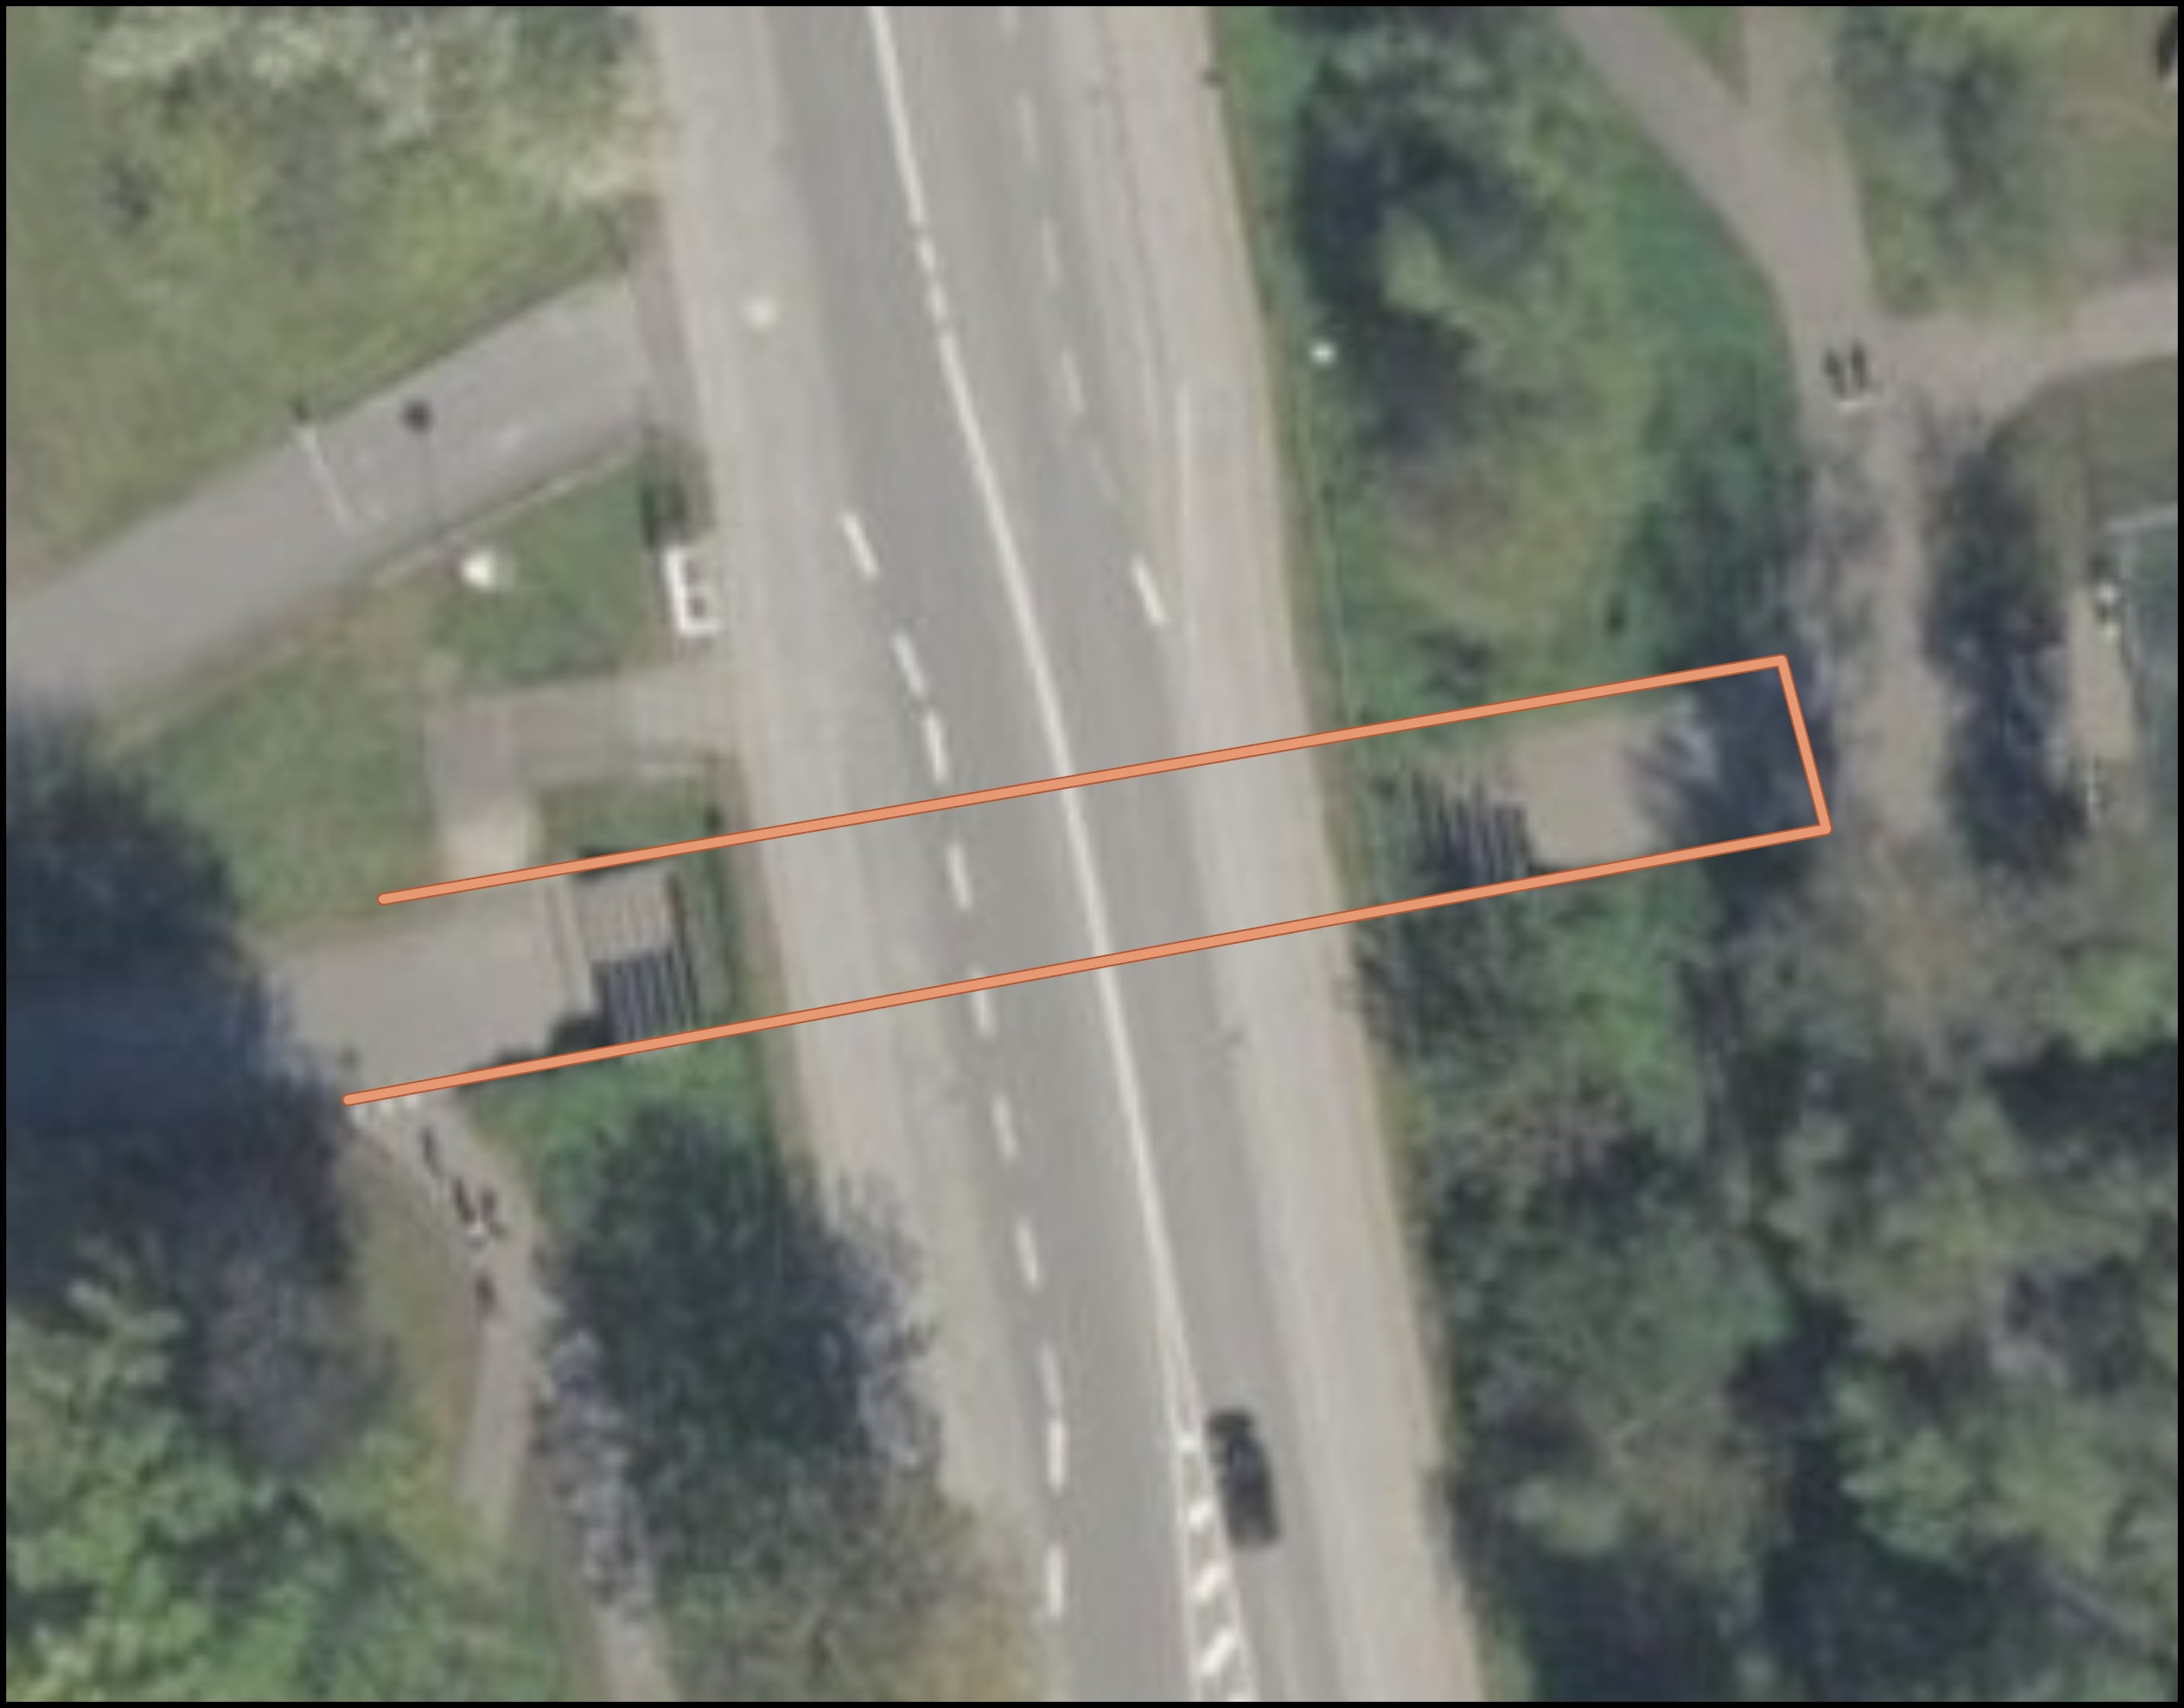
\includegraphics[width=1\linewidth]{images/databeskrivelse/hestesko.jpg}
        \caption{}
        \label{Subfig: Hesteskotilpasninger før ændring}
    \end{subfigure}
    \hspace{0.2cm}
    \begin{subfigure}[t]{0.5\textwidth}
        \centering
        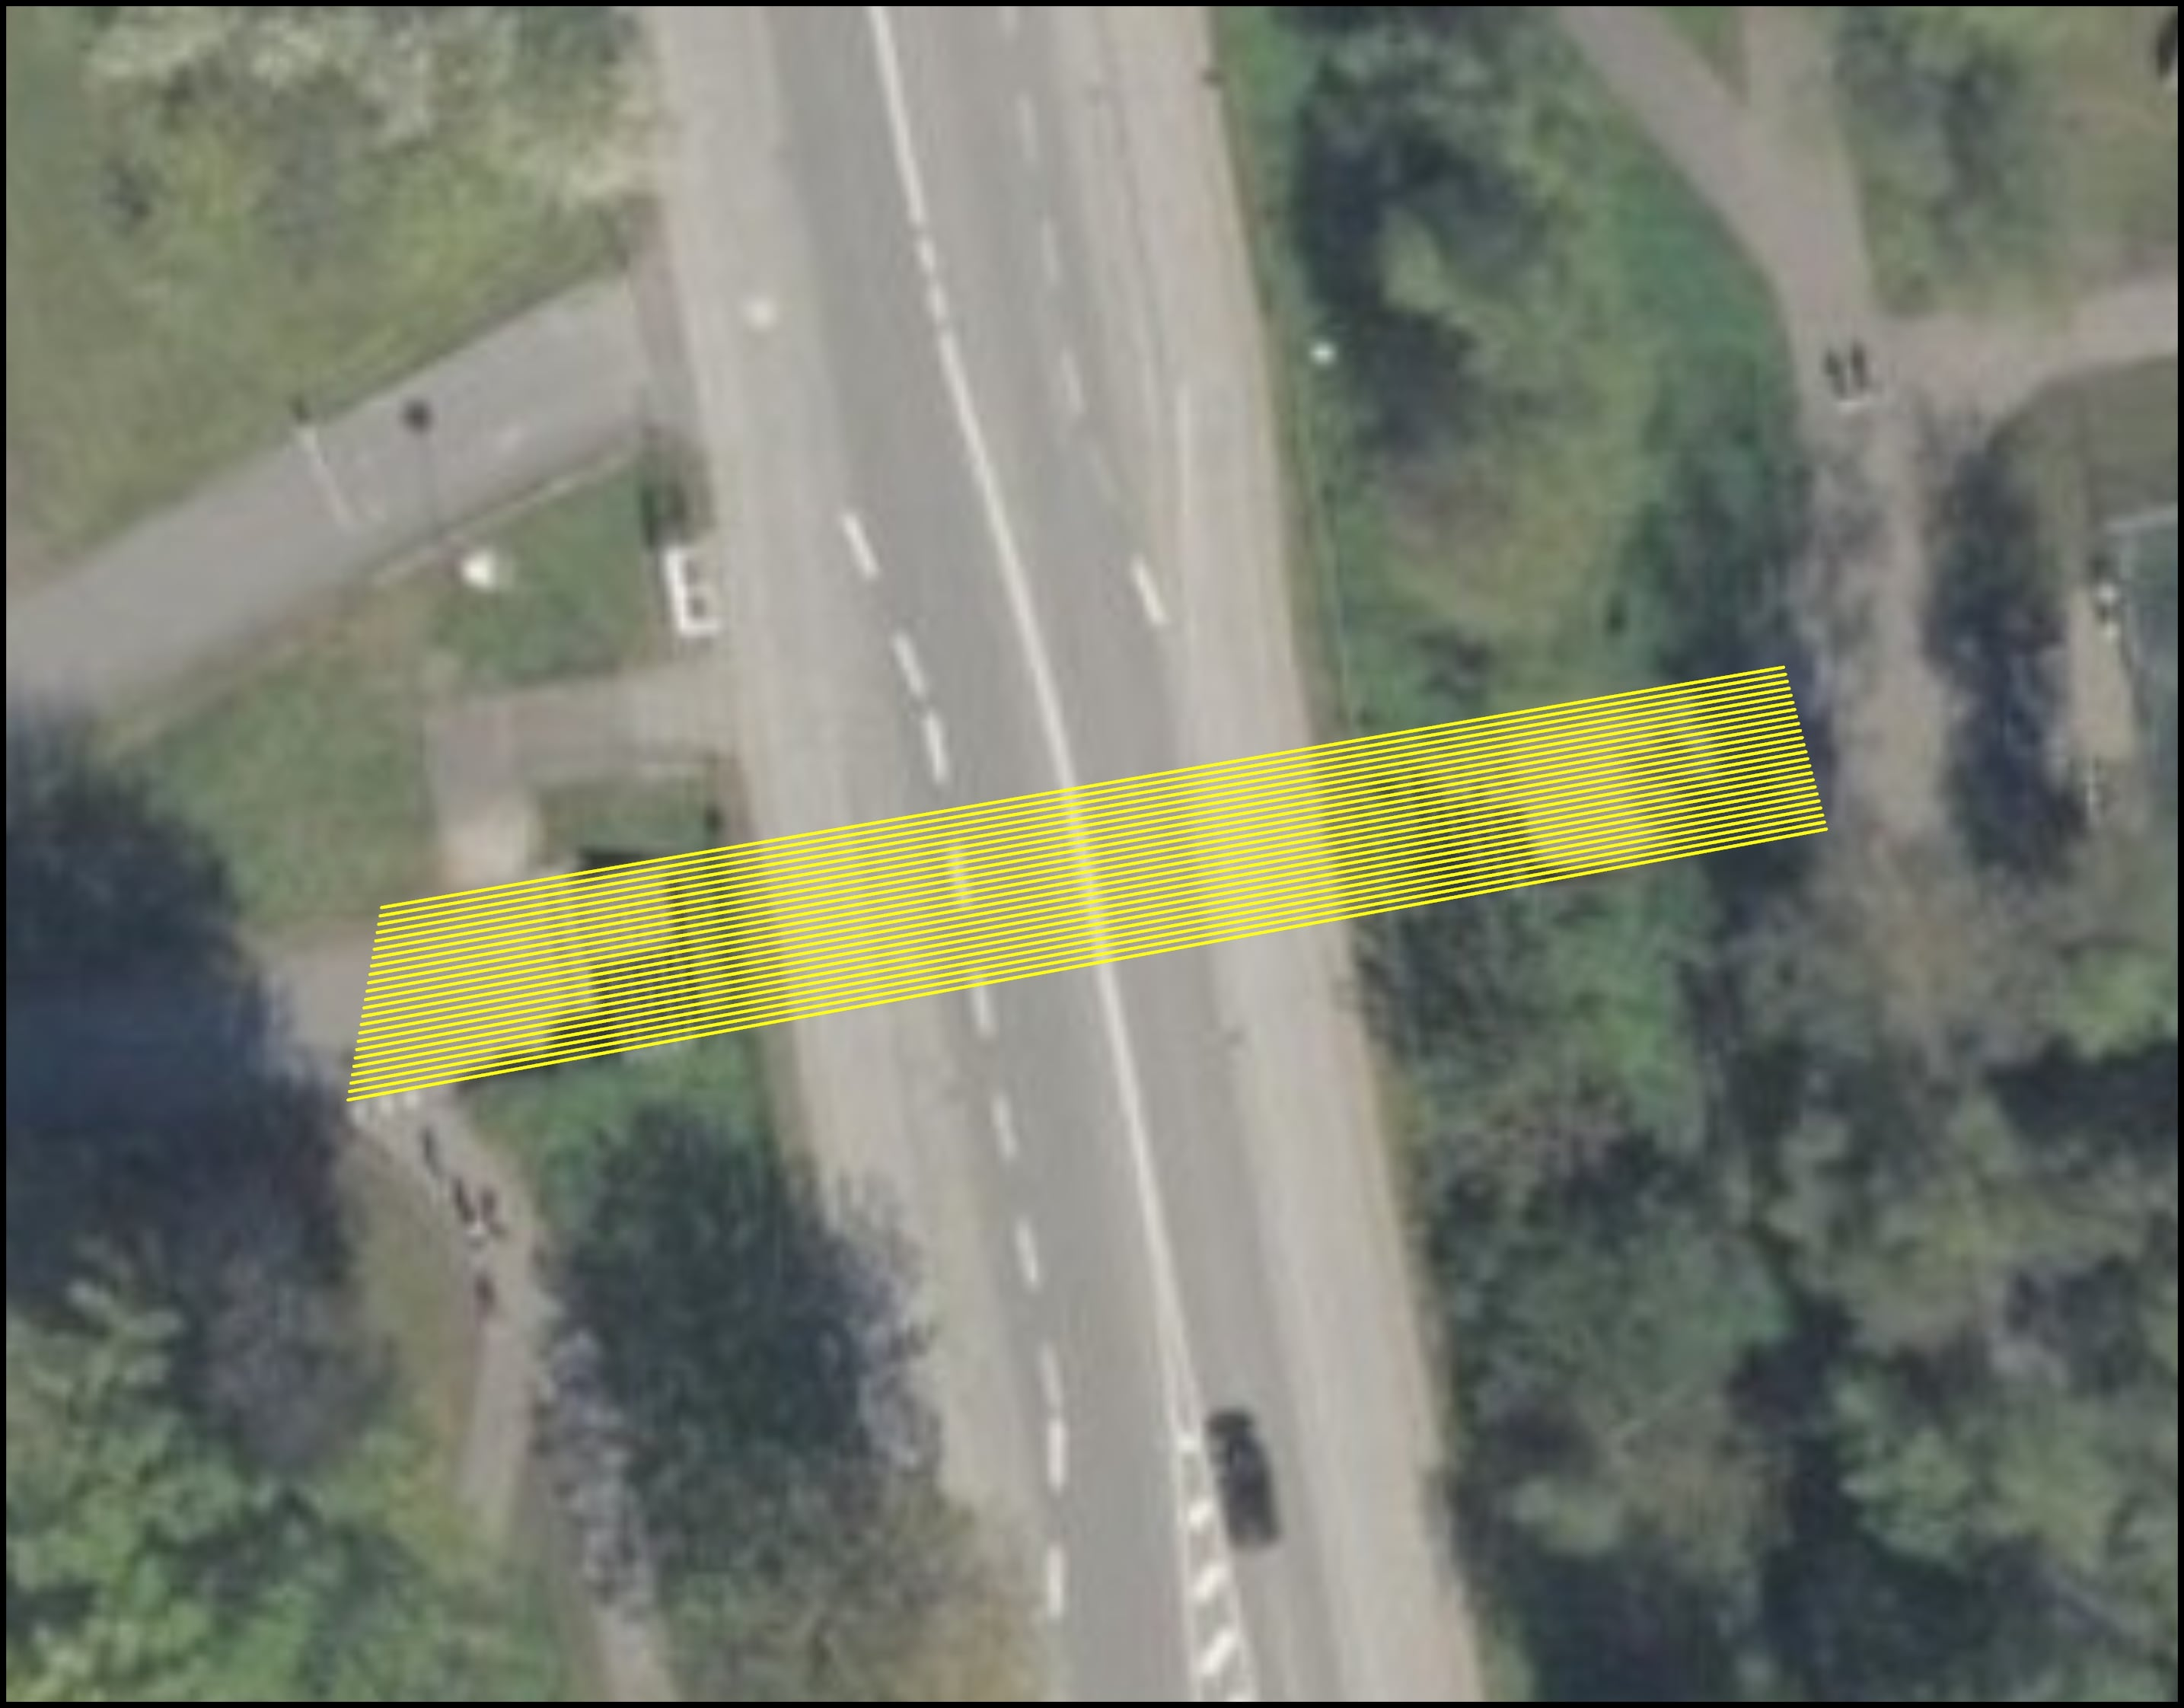
\includegraphics[width=1\linewidth]{images/metode/hestesko_linjer.jpg}
        \caption{}
        \label{Subfig: Hesteskotilpasning efter tilpasningen er konverteret til linjer}
    \end{subfigure}
    \caption{Ændringen af en hesteskotilpasning fra en hesteskoform til separate linjer. \textbf{(a)} Hesteskotilpasningen før ændring. \textbf{(b)} Hesteskotilpasningen efter tilpasningen er konverteret til linjer.}
    \label{Figur: Ændringen af hesteskotilpasningerne}
\end{figure}

Dette danner et nyt sammenlagt lag med alle de relevante hydrologiske tilpasninger som linjer. For at tilpasningen bliver korrekt repræsenteret i DHyM skal højdeværdier under terræn hindringer først interpoleres og tildeles til hver tilpasning.\\
Dette blev gjort ved at bruge et Python-script \textit{"Hydrologic Conditioning Multiple"}, som tildeler en z-værdi fra DTM til hver af linjernes endepunkter: $Z_0$ og $Z_1$. Ud fra linjernes endepunkter bliver linjens hældning, $\Delta{Z}$ udregnet ved at bruge afstanden mellem endepunkterne. Linjen konverteres til et rasterformat og derefter til punkter for hver celle i DTM. Derefter foretages der en lineær interpolation af punkterne langs linjen baseret på startpunktet $Z_0$, afstanden fra $Z_0$ til punktet og linjetilpasningens hældning, $\Delta{Z}$. Dette gøres for alle punkter langs linjen (figur \ref{Figur: Interpolation af Z-værdier}). \\

Efter z-værdierne for punkterne er blevet interpoleret, konverteres punkterne tilbage til et rasterformat, hvorefter de hydrologiske tilpasninger brændes ned i DTM ved at kombinere de interpoleret punkter med DTM. Erstatningen sker ved at tjekke for alle celler for NoData værdier i punktrasteren. Hvis værdien er NoData, så anvendes z-værdier fra DTM. Er værdien ikke NoData så erstattes z-værdien i DTM med z-værdien fra punktrasteren.
Dette skaber den korrigeret Digitale Hydrologiske Model (DHyM).

\begin{figure}[H]
    \centering
    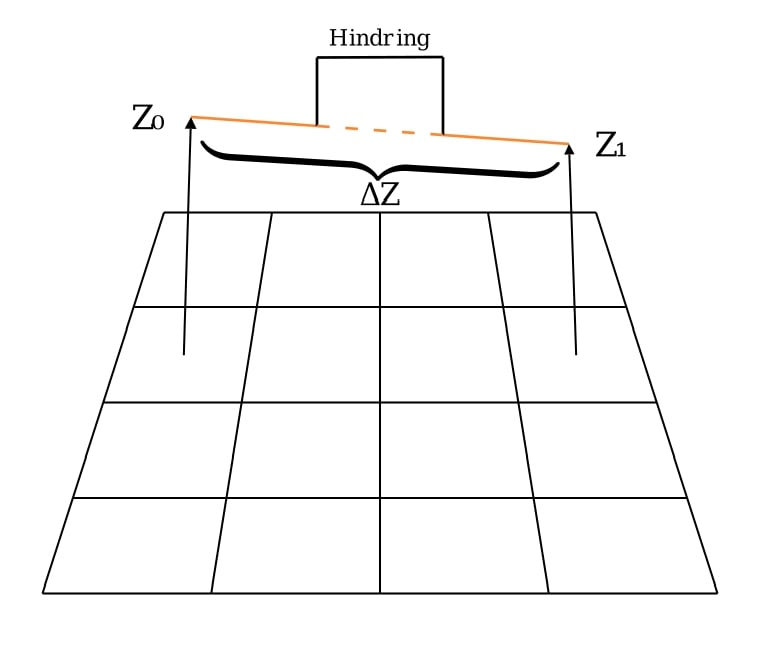
\includegraphics[width=0.5\linewidth]{images/metode/dtm_hydro_z.jpg}
    \caption{Interpolationen af z-værdier langs den orange linje for en linjetilpasning under en hindring. $Z_1$ og $Z_0$ er z-værdierne fra DTM ved linjetilpasningens endepunkter og $\Delta{Z}$ er hældningen af linjetilpasningen. Egen illustration med inspiration fra \cite{balstrom_identification_2024}}
    \label{Figur: Interpolation af Z-værdier}
\end{figure}

For studieområderne Aabenraa, Gedser Havn, Hesnæs og Præstø blev der identificeret henholdsvis 250, 13, 34 og 19 relevante hydrologiske tilpasninger, som blev brændt ned i deres tilhørende DTM.


\subsubsection{Inklusion af bygninger i DHyM} \label{Afsnit: Inklusion af bygninger i DHyM}

Efter de hydrologiske tilpasninger blev brændt ned i DTM, blev der besluttet at inkludere bygninger i DHyM, som en ikke-gennemtrængelige barrierer i terrænet. Denne beslutning blev truffet med udgangspunkt i, at de oversvømmelseskort studiekommunerne havde leveret, behandlede bygninger som barrierer. Desuden blev det vurderet at en realistisk simulering af hydrologisk adfærd forudsætter, at vand ikke kan strømme direkte igennem bygninger, men ledes udenom. \\

Metoden for at implementere bygninger i DHyM blev gennemført ved brug af \textit{"Building Block (BB)"} metoden anvendt i \cite{khosh_bin_ghomash_technical_2024}. Metoden hæver terrænhøjden i højdemodellen for hver bygningspolygoners fodaftryk til en bestemt højde. Denne højde blev arbitrært sat til 20 meter for alle bygningerne. Herefter blev bygningspolygonerne konverteret til et rasterformat med den samme cellestørrelse på 40\times40 cm som DHyM. \\
Derefter udføres der et tjek på den nye bygningsraster, hvor celler med en højdeværdi på 20 forblev 20 og celler med NoData blev tildelt værdien 0. Dette sikrer at bygningsrasteren kan kombineres med DHyM, da aritmetiske operationer på NoData-værdier ikke er muligt. Til sidst blev bygningsrasteren og DHyM lagt sammen, hvilket skabte den endelige DHyM, som anvendes i Inundation Modellen.


\subsection{Simulering af 2023-stormfloden}\label{Afsnit: Simulering af stormflod 2023}

Efter DTM er blevet konverteret til en DHyM er det muligt at udføre stormflodsmodellering via Inundation Modellen. I modellen inputtes der for hvert studieområde den tilhørende DHyM og kildelinjen \textit{"Line at Sea"}. Line At Sea linjen er manuelt digitaliseret i hvert studieområde ude i havet.\\ 
Hvert studieområde simuleres op til det højeste officielle vandstandsniveau målt ved oktober 2023 stormfloden og antallet af iterationer for at opnå dette niveau er vist i tabel \ref{Tabel: Antal iterationer og slutværdier for Inundation Model}. Alle studieområder starter oversvømmelsessimuleringen med en startværdi på  100 cm og en vandstandsstigningsværdi på 1 cm. En startværdi på 100 cm blev valgt primært på grund af processeringstid og vandstandsstigningsværdien på 1 cm blev valgt for at opnå størst fleksibilitet og gjorde det muligt at opnå nøjagtig samme vandstandsniveau som målt under stormfloden. Simuleringstiden for hver af de fire studieområder er vist i tabel \ref{Tabel: Antal iterationer og slutværdier for Inundation Model} og sammenlagt tog det 12 timer og 1 minut at simulere 2023-stormfloden ved for de fire studieområder.\\
\begin{table}[H]
\centering
\renewcommand{\arraystretch}{1}
\begin{threeparttable}
\caption{Antal iterationer, slutværdien og processeringstiden for oversvømmelsessimuleringer i Inundation Modellen for simulere oktober 2023 stormfloden}
\begin{tabular}{@{} l 
                S[table-format=7.2, output-decimal-marker={,}] 
                S[table-format=7.2, output-decimal-marker={,}]
                l @{}} 
\toprule
\textbf{Lokalitet} & \textbf{Antal iterationer} & \textbf{Slutværdi (cm)}  & \textbf{Simuleringstid}\\
\midrule
Aabenraa & 117 & 216 & 5 timer 27 minutter \\
Gedser & 90 & 189 & 3 timer 25 minutter\\ 
Hesnæs & 111 & 210 & 1 time 23 minutter \\
Præstø & 101 & 200 & 1 time 44 minutter \\
\bottomrule
\end{tabular}
\label{Tabel: Antal iterationer og slutværdier for Inundation Model}
\end{threeparttable}
\end{table}

Efter simulgeringen er færdig er der blevet produceret en raster for hver centimeter fra startværdien på 100 til slutværdien. Hver inundationraster viser hvilken vandstand alle celler i rasteren bliver oversvømmet ved. Herefter blev der brugt et intern ArcGIS Pro værktøj \textit{"Cell Statistics"} til at finde den minimums vandstand for alle celler i alle rasterlag og kombinere dem sammen til en samlet raster. Denne raster blev filtreret med en landpolygon, så det kun er oversvømmelse på land der bliver medtaget i det endelige resultat af simuleringen. Dette gøres fordi modellen teknisk set simulerer oversvømmelse fra havet til kysten udfra Line At Sea-linjen. Ved at bruge landpolygonen fjernes de ekstra unødvendige værdier fra resultatet.\\
Dette gøres for alle fire studieområder og producerer dermed de fire simulerede oversvømmelseskort over 2023-stormfloden der sammenlignes med de kort hver kommune leverede over vandets udbredelse observeret under stormfloden.  


\subsection{Kvantificering af påvirkede areal anvendelser} \label{Afsnit: Udregning af påvirkede areal anvendelser}

For at kvantificere stormfloden i 2023s påvirkning af studieområderne blev der gennemført en krydstabulering mellem arealanvendelses datasættet fra BaseMap04 og både de observerede samt simulerede oversvømmelser forårsaget af stormfloden.\\

Indledningsvis blev BaseMap04-arealanvendelsesrasteren, som oprindeligt har en cellestørrelse på 10\times10 meter resamplet til en cellestørrelse svarende til outputtet fra Inundation Modellen (40\times40 cm). Herefter blev ArcGIS Pro-værktøjet \textit{"Tabulate Area"} anvendt til at beregne det oversvømmede areal for hver arealanvendelsesklasse, for både observerede data og modellens resultater.
 
\begin{figure}[H]
    \centering
    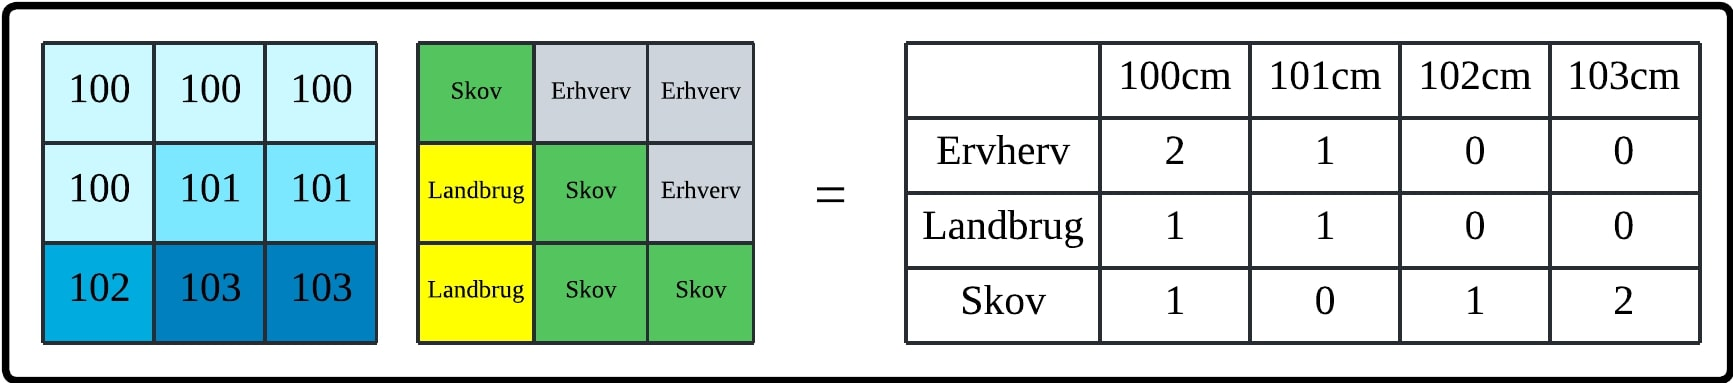
\includegraphics[width=1\linewidth]{images/metode/tabulate.jpg}
    \caption{Krydstabulerings processen bag Tabulate Area værktøjet i ArcGIS Pro. Hver celle i oversvømmelsesrasteren kobles til en celle i arealanvendelsesrasteren og tabuleres. Egen illustration med inspiration fra \cite{esri_tabulate_nodate}}
    \label{Figur: Tabulate}
\end{figure}
Værtøjet Tabulate Area krydsreferer hver celle i BaseMap-arealanvendelsesrasteren med den tilsvarende celle i oversvømmelsesrasteren, således at der knyttes en specifik arealanvendelse til et givent oversvømmelsesniveau. Dette muliggør en kvantitativ vurdering af stormflodens påvirkning på forskellige arealanvendelser i studieområderne (figur \ref{Figur: Tabulate}).\\

Resultatet af krydstabuleringen præsenteres i form af en kontingenstabel, hvor rækkerne repræsenterer de forskellige arealanvendelsesklasser, og kolonner angiver de respektive oversvømmelsesnivauer i centimeter. Ud fra denne tabel summeres antallet af celler for hver unik arealanvendelse, hvorefter det samlede oversvømmede areal for her klasse beregnes som en andel af det totale oversvømmede areal. Resultatet visualiseres efterfølgende i form af søjlediagrammer.

\subsection{Fremskrivning af 2023 stormfloden og en statistisk 100-års hændelse} \label{Afsnit: Fremskrivning og statistisk}
I lyset af fremtidige klimaforandringer og risikoen for stigende vandstand i Danmark, undersøges der hvordan hvordan en oversvømmelse vil se ud ved to forskellige hændelser: et statistisk oversvømmelsesniveau ved en 100-års hændelse og en fremskrivning af hvordan 2023-stormfloden til slutningen af det nuværende århundrede vil se ud baseret på vandstandsprojektioner fra den sjette \cite{ipcc_report_AR6} rapport. For begge hændelsestyper simuleres der for to forskellige Shared Socioeconomic Pathways (SSP) scenarier: et mellemhøjt udledningsscenarie (SSP2-4,5) og et meget højt udledningsscenarie (SSP5-8,5). Det mellemhøje scenarie blev valgt som en kompromisbaseret mellemposition mellem det højeste mulige klimascenarie og det mildeste, selvom \cite{dmi_ny_nodate} understreger, at kommunerne og forvaltningsinteressenter bør bruge det høje scenarie (SSP3-7) i klimavurderinger. Det meget høje scenarie blev valgt for at simulere en stormflod under det værst mulige udfald på baggrund af socioøkonomiske faktorer.\\

{\large \textit{Statistisk 100-års hændelse}}\\
For at undersøge påvirkningen af studieområderne baseret på en statistisk 100-års hændelse, blev DMIs Klimaatlas anvendt til at bestemme vandstandshøjden af en stormflod der statistisk set vil optræde en gang per 100 år. Klimaatlas inddeler Danmarks kyster i kyststrækninger og de fire kyststrækninger der blev anvendt er: Lillebælt Syd for Aabenraa, Femern Bælt for Gedser, Falsters og Møns Østersøkyst for Hesnæs og Faxe Bugt for Præstø. For hver kyststrækning anvendes den absolute vandstandshøjde for en 100-års hændelse ved SSP2,5-4,5 og SSP5-8,5.\\

Herefter bruges Inundation Modellen til at simulere op til SSP5-8,5 scenariet for hvert studieområde. Processen bag dette er den samme som i afsnit \ref{Afsnit: Simulering af stormflod 2023}, men i stedet for at starte ved 100 cm starter modellen ved den observerede vandstandshøjde ved stormfloden for hvert studieområde. Der blev simuleret op til en vandstandshøjde på 251 cm for Aabenraa, 242 cm for Gedser, 253 cm for Hesnæs og 225 cm for Præstø og tilføjede sammenlagt en ekstra 2 timer og 46 minutter i simuleringstid. \\

{\large \textit{Fremskrivning af 2023-stormfloden}} \\
Da vandstanden i Danmark forventes at stige i løbet af det nuværende århundrede har det derfor været ønsket at se hvordan 2023 stormflodshændelsen vil se ud hvis den skete i slutningen af århundredet. Til at gøre dette er der lavet en beregning af middelvandstanden i 2100. DMIs Klimaatlas har allerede værdier for middelvandstanden i 2100, men deres værdier er i forhold til en referenceperiode fra 1981-2010. Det har derfor været nødvendige at beregne middelvandstandsniveauet i 2023 i forhold til DMIs referenceperiode og derefter beregne hvad middelvandstanden vil være i 2100 baseret på vandstanden i 2023.\\ 

Til at udføre denne udregning er der blevet anvendt et datasæt fra \cite{garner_ipcc_2021} over havspejlsprojektioner og et online værktøj udarbejdet af \cite{NASA_tool}. NASAs værktøj gør det muligt at få projektioner til en bestemt Permanent Service for Mean Sea Level (PSMSL) station. I værktøjet vælges den nærmeste PSMSL-station for hvert område. Stationen blev udvalgt ud fra hvilket hav basin, der var tættest på hvert område. Dette var Fynshav for Aabenraa, Gedser Havn for Gedser, Warnemünde for Hesnæs og Skanör for Præstø.\\ 

Værktøjet giver derefter en tabel med alle de individuelle bidrag til havspejlsstigning og en median havspejlsstigning ($SLR_{50}$) for hver station i forhold til en referenceperiode fra 1995-2014. $SLR_{50}$ indeholder en række faktorer der påvirker havspejlsstigning, såsom ferskvandstilførsel fra floder, glacial bidrag og tager højde for lokal isostasi. For at udregne middelvandstanden i 2023, er projektionen for 2030 anvendt, da det er den tætteste. Til udregningen er der blevet opstillet en følgende ligning: 
\begin{align} \label{Equation: Vandstandsstigning calculation}
    S_r = S_p- \left( \frac{\Delta{t}}{\Delta{t_r}}\times SLR_{50} + \Delta{M_r} \times \left(\frac{SLR_{50}}{\Delta{t_r}}\right) \right)
\end{align}
Middelvandstanden i 2023 beregnes ved at finde forholdet af differencen mellem målåret fx 2023 ($\Delta{t}$), NASAs referenceår ($\Delta{t_r}$) og projektionsåret. Dette forhold ganges med $SLR_{50}$ og giver middelvandstanden i 2023 i forhold til NASAs referenceperiode 1995-2014. Herefter beregnes den forventede middelvandstandsstigning fra DMIs referenceperiode (1981-2010) til NASAs referenceperiode (1995-2014). Denne udregning er lavet med den antagelse at stigningen fra DMIs referenceperiode til NASAs reference har været lineær \citep{danish_meteorological_institute_dmi_2024}. Dette gøres ved at tage differencen mellem referenceperiodernes median år ($\Delta{M_r}$) og gange med raten af havspejlstigning ($\frac{SLR_{50}}{\Delta{t_r}}$) frem mod 2030. \\
Dette giver et resultat for hvad middelvandstanden i 2023 har været i forhold til DMIs referenceperiode og gør det muligt at fratrække denne vandstand fra den projekteret vandstand i slutningen af det nuværende århundrede ($S_p$) og giver $S_r$ som er middelvandstanden i slutningen af århundredet med 2023 som det nye referenceår. Denne fremgangsmåde blev udført ved et SSP2-4,5 og et SSP5-8,5 scenarie.\\

Herefter blev Inundation Modellen igen kørt for at få nye oversvømmelsesdata. Der blev simuleret op til 268 cm for Aabenraa, 259 for Hesnæs og 246 for Præstø. Der blev ikke simuleret nye oversvømmelser for Gedser da 100-års hændelsen ved SSP8.5 er en højere vandstand end den fremskrevet 2023 stormflod til slutningen af århundredet. Fremskrivningen tilføjede en yderlig 1 time og 58 minutter til samlet simuleringstid.\\


Derefter blev alle oversvømmelsesrasterne konverteret til polygoner og kombineret med værktøjet \textit{"Merge"} for at få visualiseret forskellene mellem en 100-års hændelse og en fremskrivning af stormfloden på et samlet kort.


\newpage
\section{Resultater}

På baggrund af simuleringer med Inundation Modellen og analysering af resultaterne præsenteres resultaterne af 2023-stormflods simuleringen, påvirkede arealanvendelser og simuleringerne af fremtidige klimascenarier på baggrund af en statistisk 100-års hændelse og en fremskrevet stormflod ved et SSP4,5 og 8,5 udledningsscenarie. 

\subsection{Simuleringen af 2023-stormfloden}
Figur \ref{Subfig: Målt Aabenraa} viser det oversvømmelseskort Aabenraa kommune har udarbejdet, der viser den observerede hændelse fra stormfloden og figur \ref{Subfig: Model Aabenraa} viser resultatet af simuleringen af stormfloden fra Inundation Modellen for Aabenraa. \\
Der er forskel mellem de to resultater. Modellens resultat er større især vest for lystbådehavnen ved et større rekreativt område og et bebygget område. Modellen resulterede i et areal på 129,8 ha, mens det observeret areal var på 70,1 ha. Dette medfører i at modellens resultat er 83,5\% større end den observeret hændelse, svarende til ca. 59 ha.
\begin{figure}[H]
    \begin{subfigure}[t]{0.5\textwidth}
        \centering
        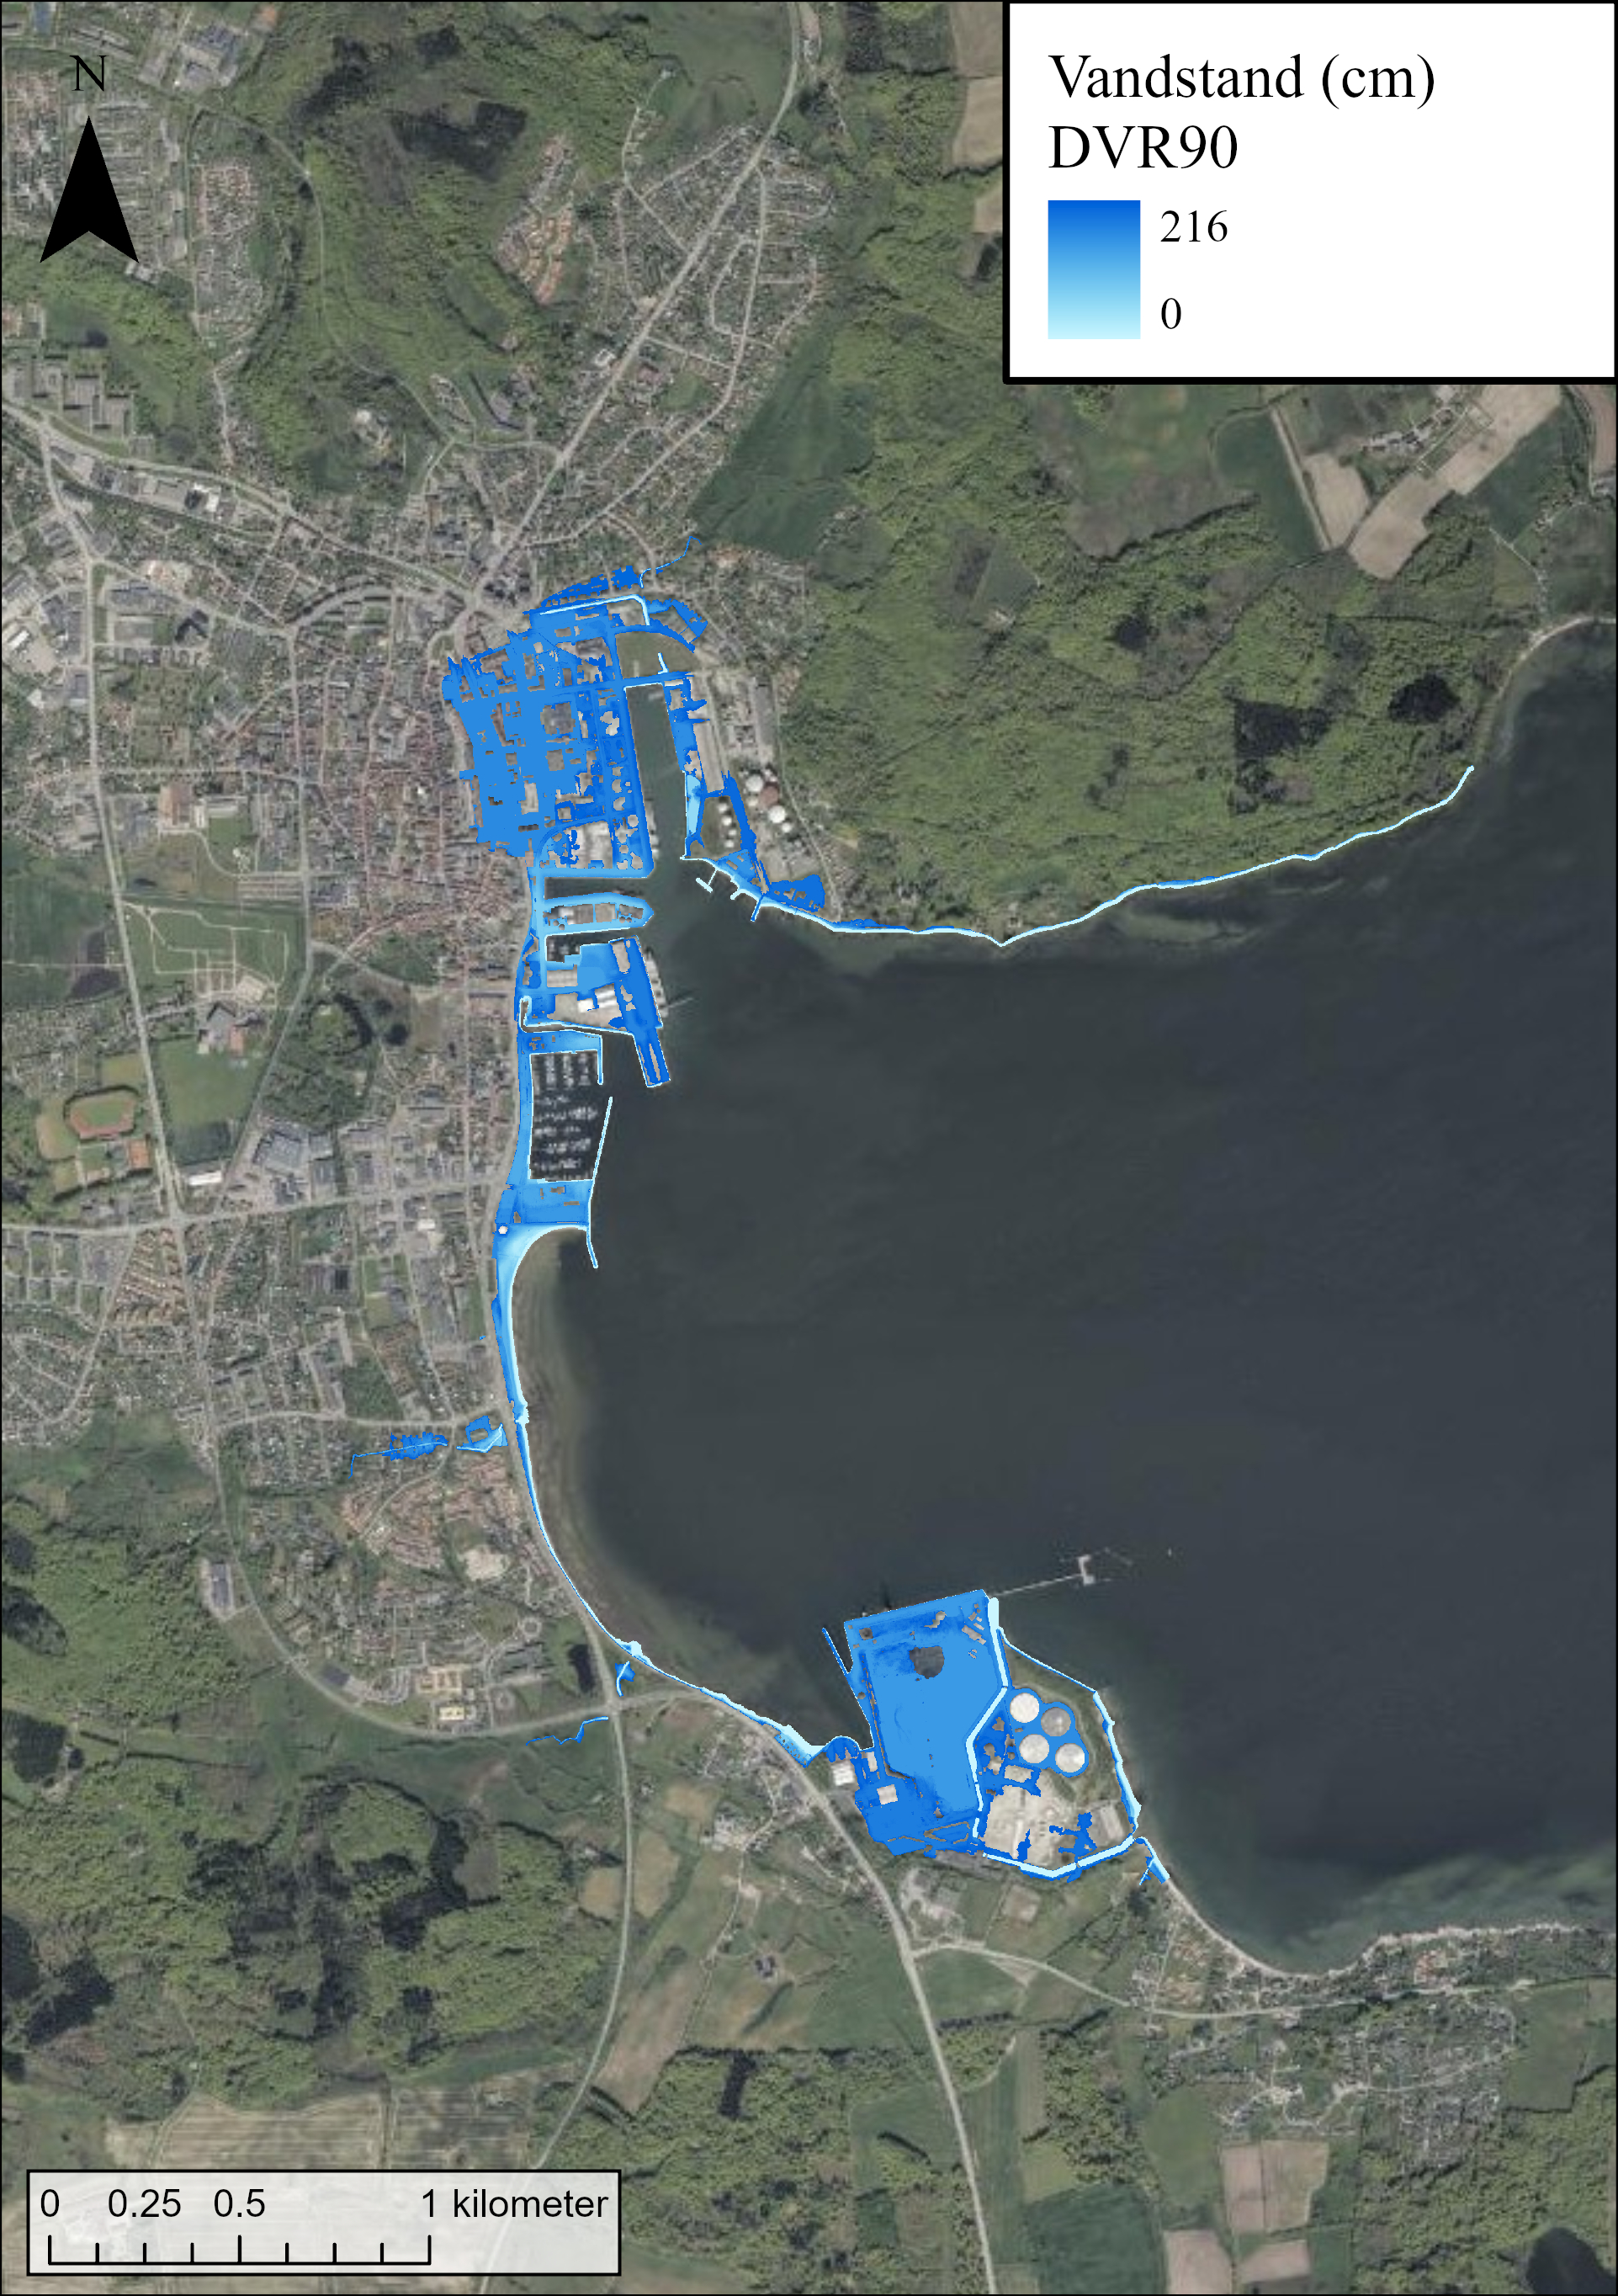
\includegraphics[width=0.95\linewidth]{images/Resultater/2023Malt/2023 resultat_aabenraa.jpg}
        \caption{}
        \label{Subfig: Målt Aabenraa}
    \end{subfigure}
    \begin{subfigure}[t]{0.5\textwidth}
        \centering
        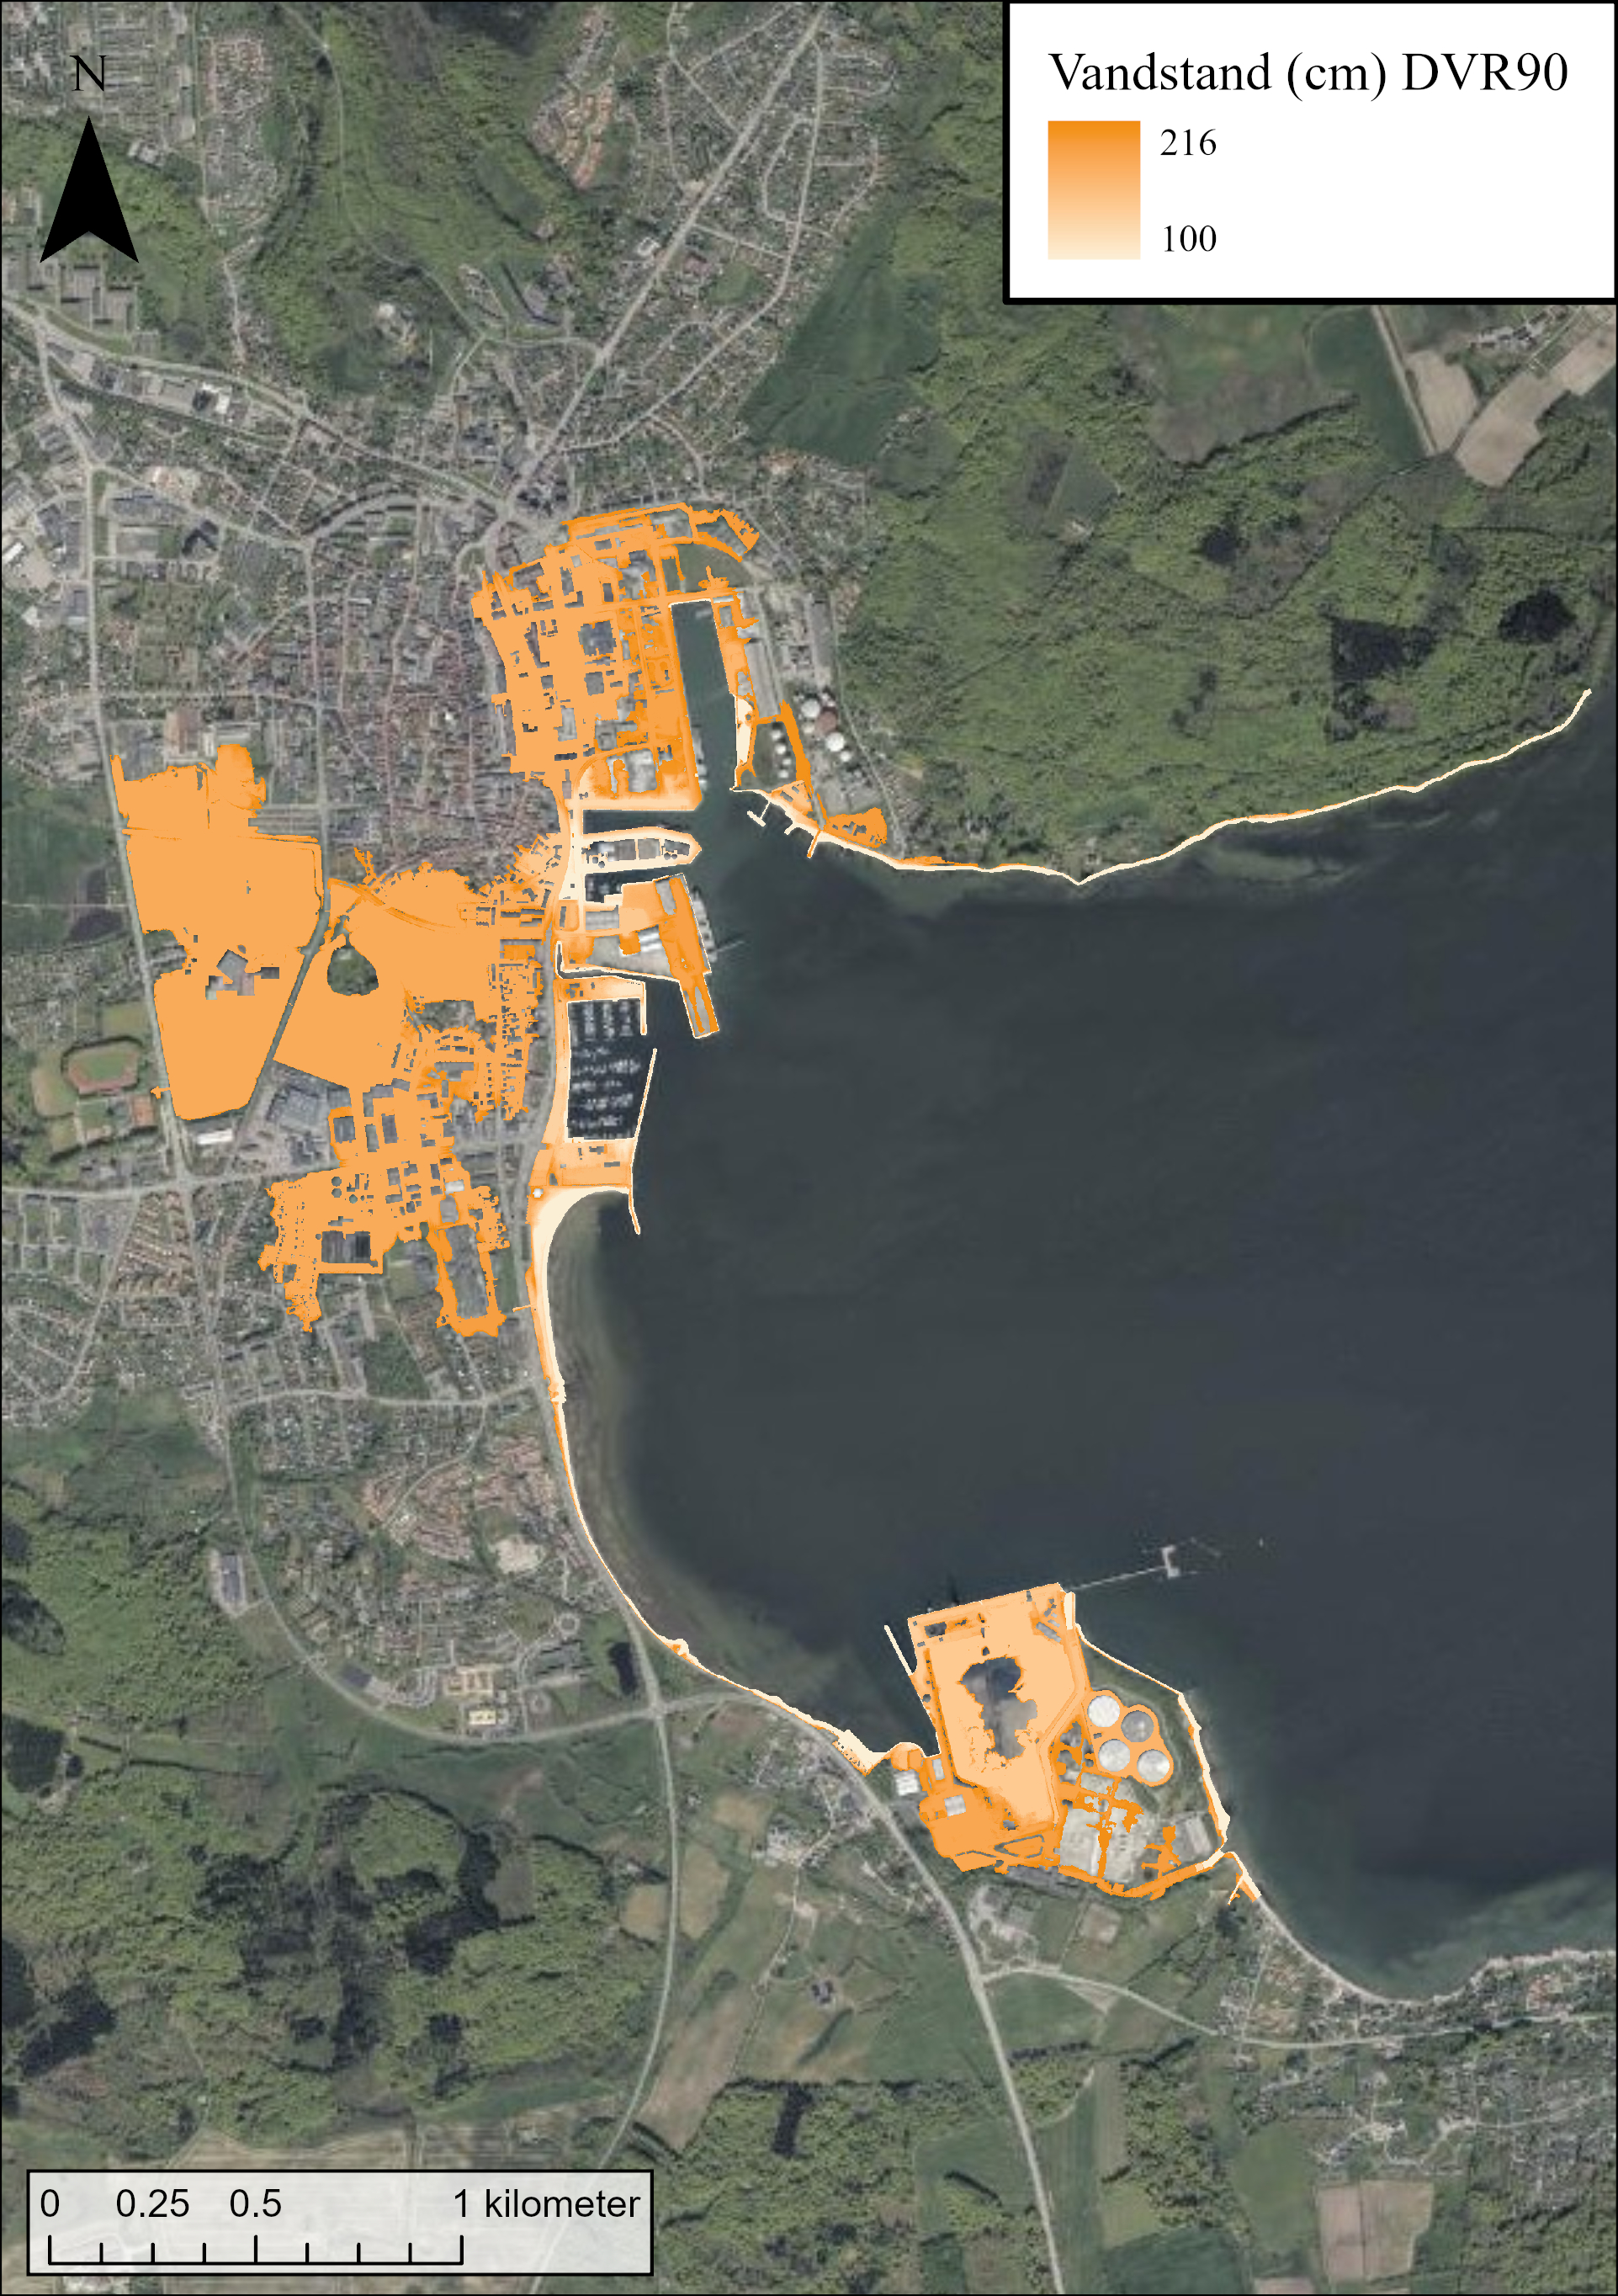
\includegraphics[width=0.95\linewidth]{images/Resultater/2023Model/2023 model_aabenraa.jpg}
        \caption{}
        \label{Subfig: Model Aabenraa}
    \end{subfigure}
    \caption{Oversvømmelseskort over 2023-stormfloden for Aabenraa. \textbf{(a)} Observeret data \textbf{(b)} Simuleret data.}
    \label{Figur: Målt & simuleret Aabenraa}
\end{figure}
Stormfloden i Aabenraa påvirkede syv forskellige arealanvendelser. I figur \ref{Subfig: Arealklasser i procent Aabenraa} er der vist hvilke arealer der blev påvirket under den observeret og simuleret stormflod, som procent af det totale oversvømmet areal. Under den observeret stormflod blev 42\% af bebyggede områder oversvømmet, svarende til 30 ha (figur \ref{Subfig: Hektar arealklasser Aabenraa}). Hvorimod ved den simuleret stormflod blev 29\% af det bebyggede areal oversvømmet, svarende til ca. 37 ha (figur \ref{Subfig: Hektar arealklasser Aabenraa}). En anden klasse hvor der er forskel mellem resultaterne er rekreativt areal, hvor 25 ha oversvømmes i den simuleret stormflod, svarende til ca. 20\% af det totale areal. I modsætning til den observeret stormflod hvor 0,41 ha (0,6\%) af rekreativ areal blev oversvømmet.
\begin{figure}[H]
    \begin{subfigure}[t]{0.5\textwidth}
        \centering
        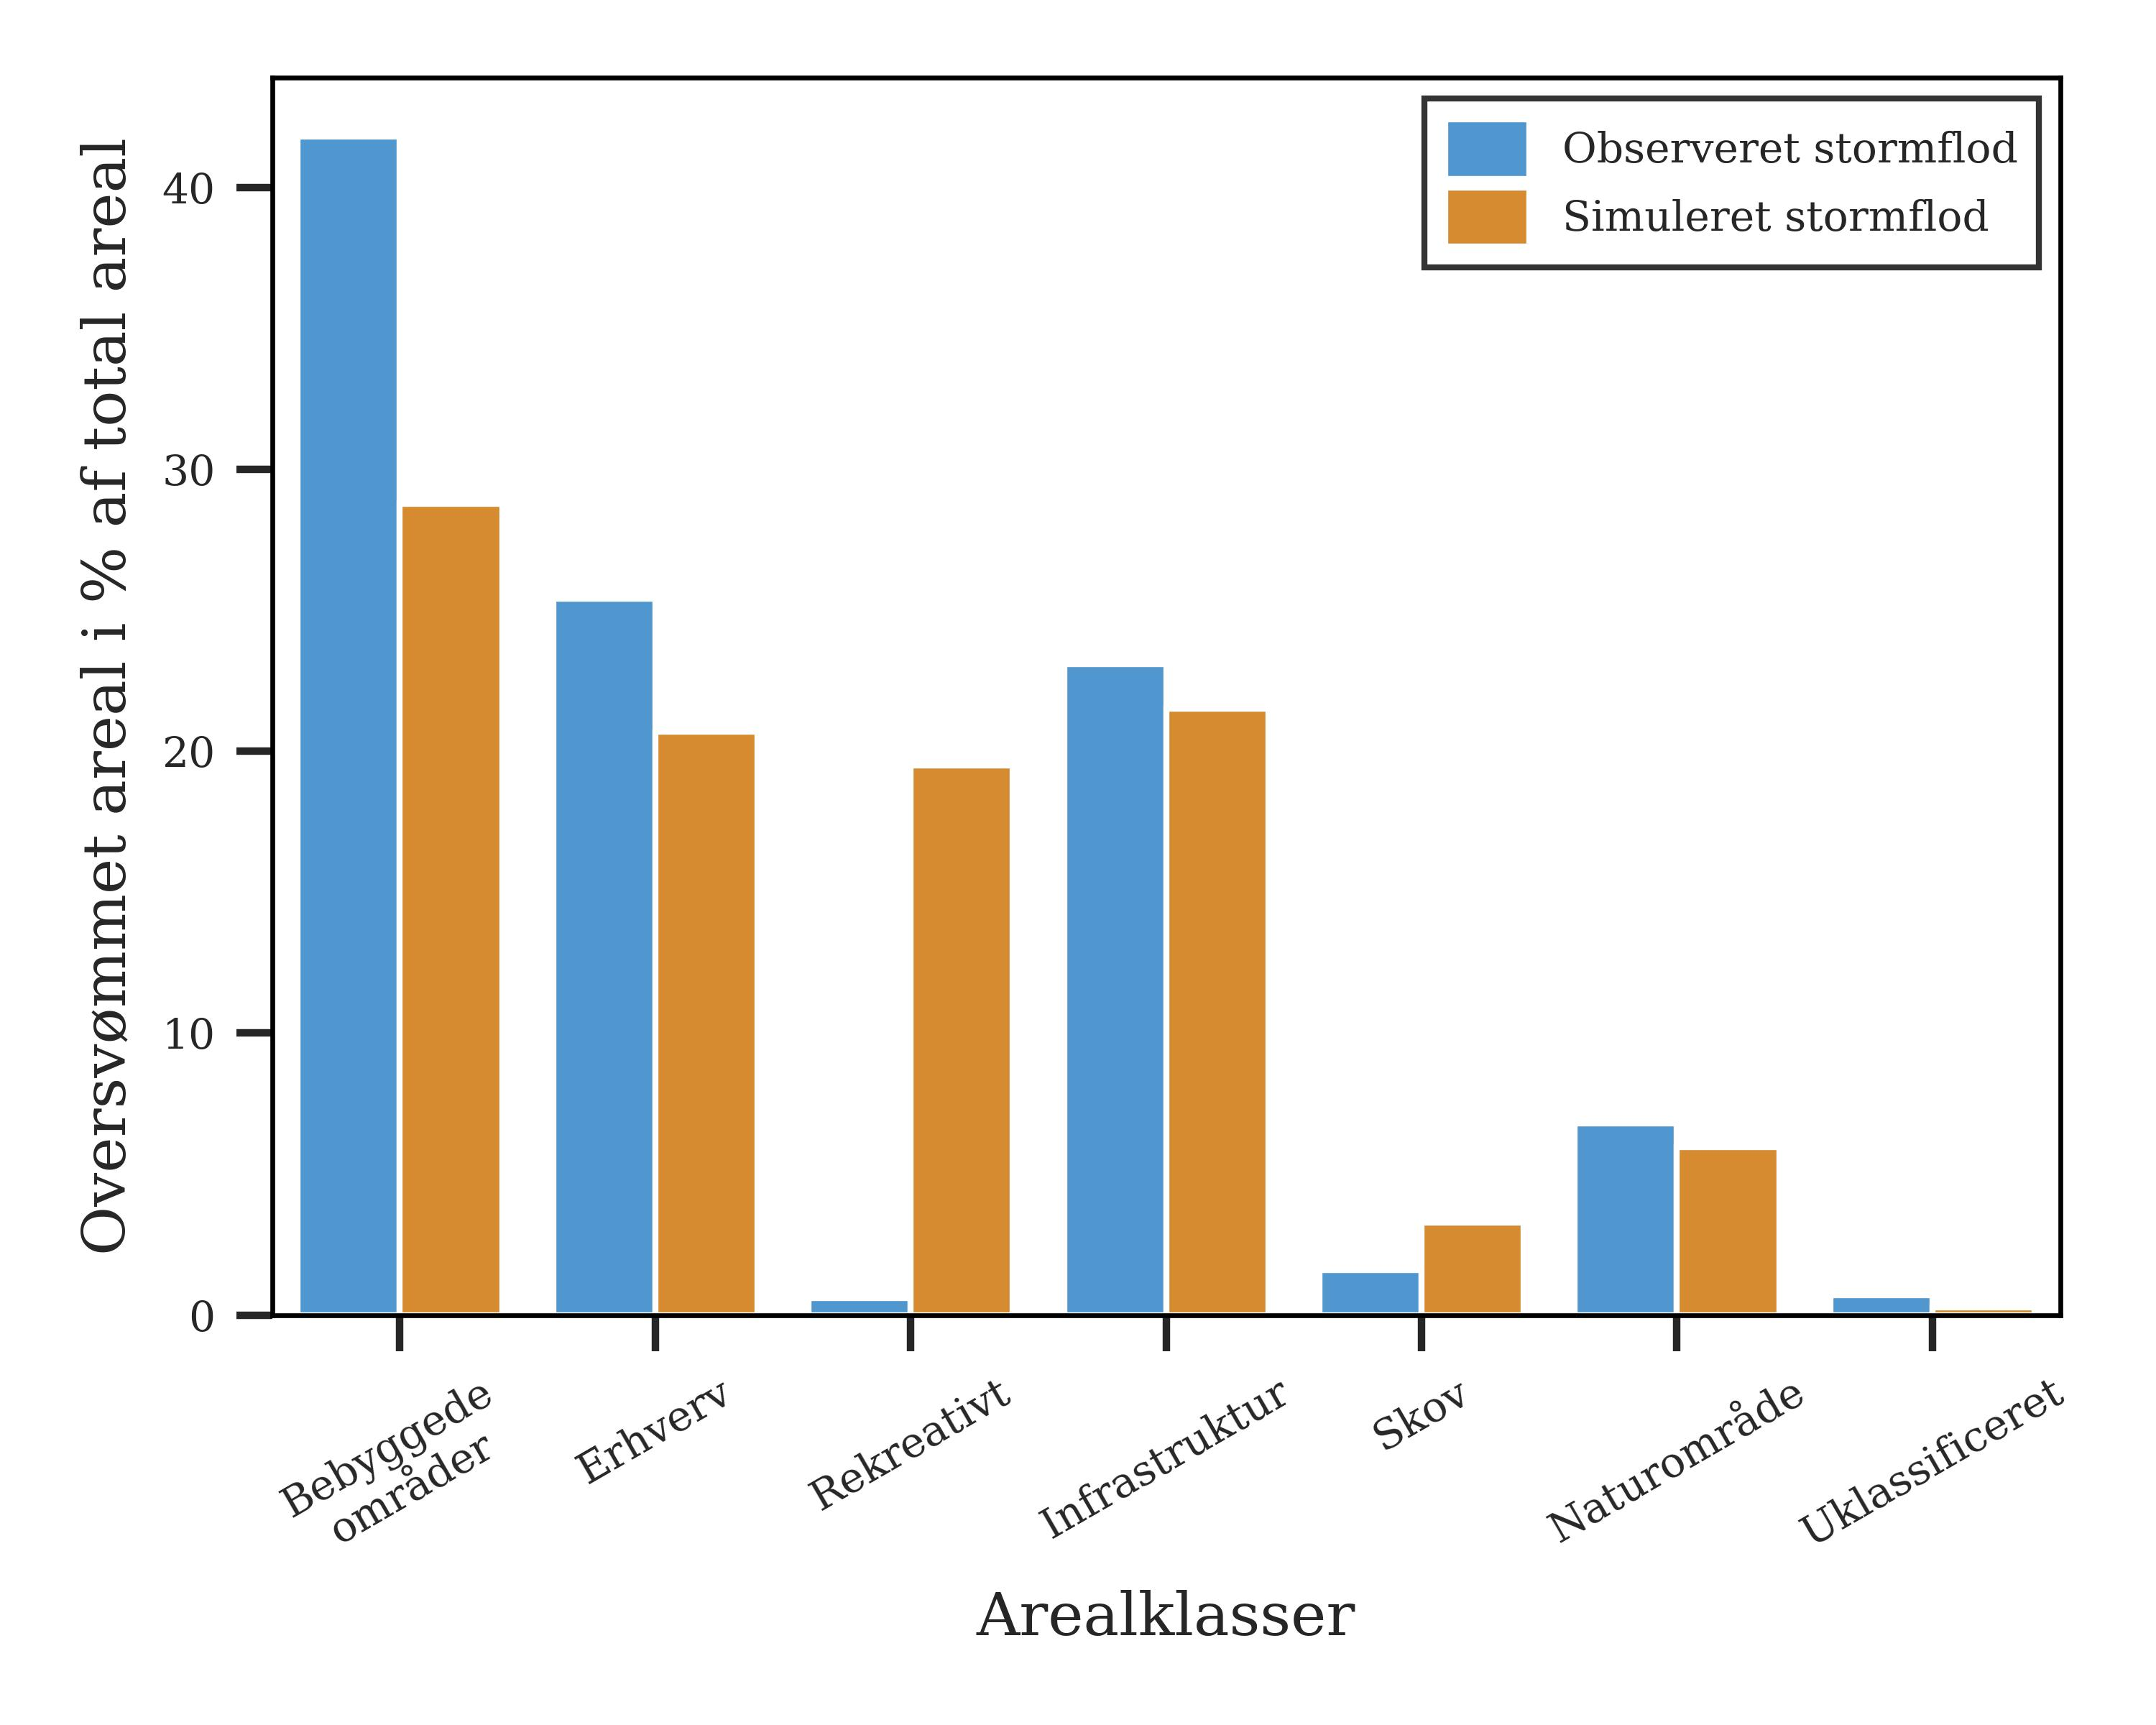
\includegraphics[width=1\linewidth]{images/Resultater/areal_anvendelses_grafer/aabenraa_arealanvendelse.jpg}
        \caption{}
        \label{Subfig: Arealklasser i procent Aabenraa}
    \end{subfigure}
    \begin{subfigure}[t]{0.5\textwidth}
        \centering
        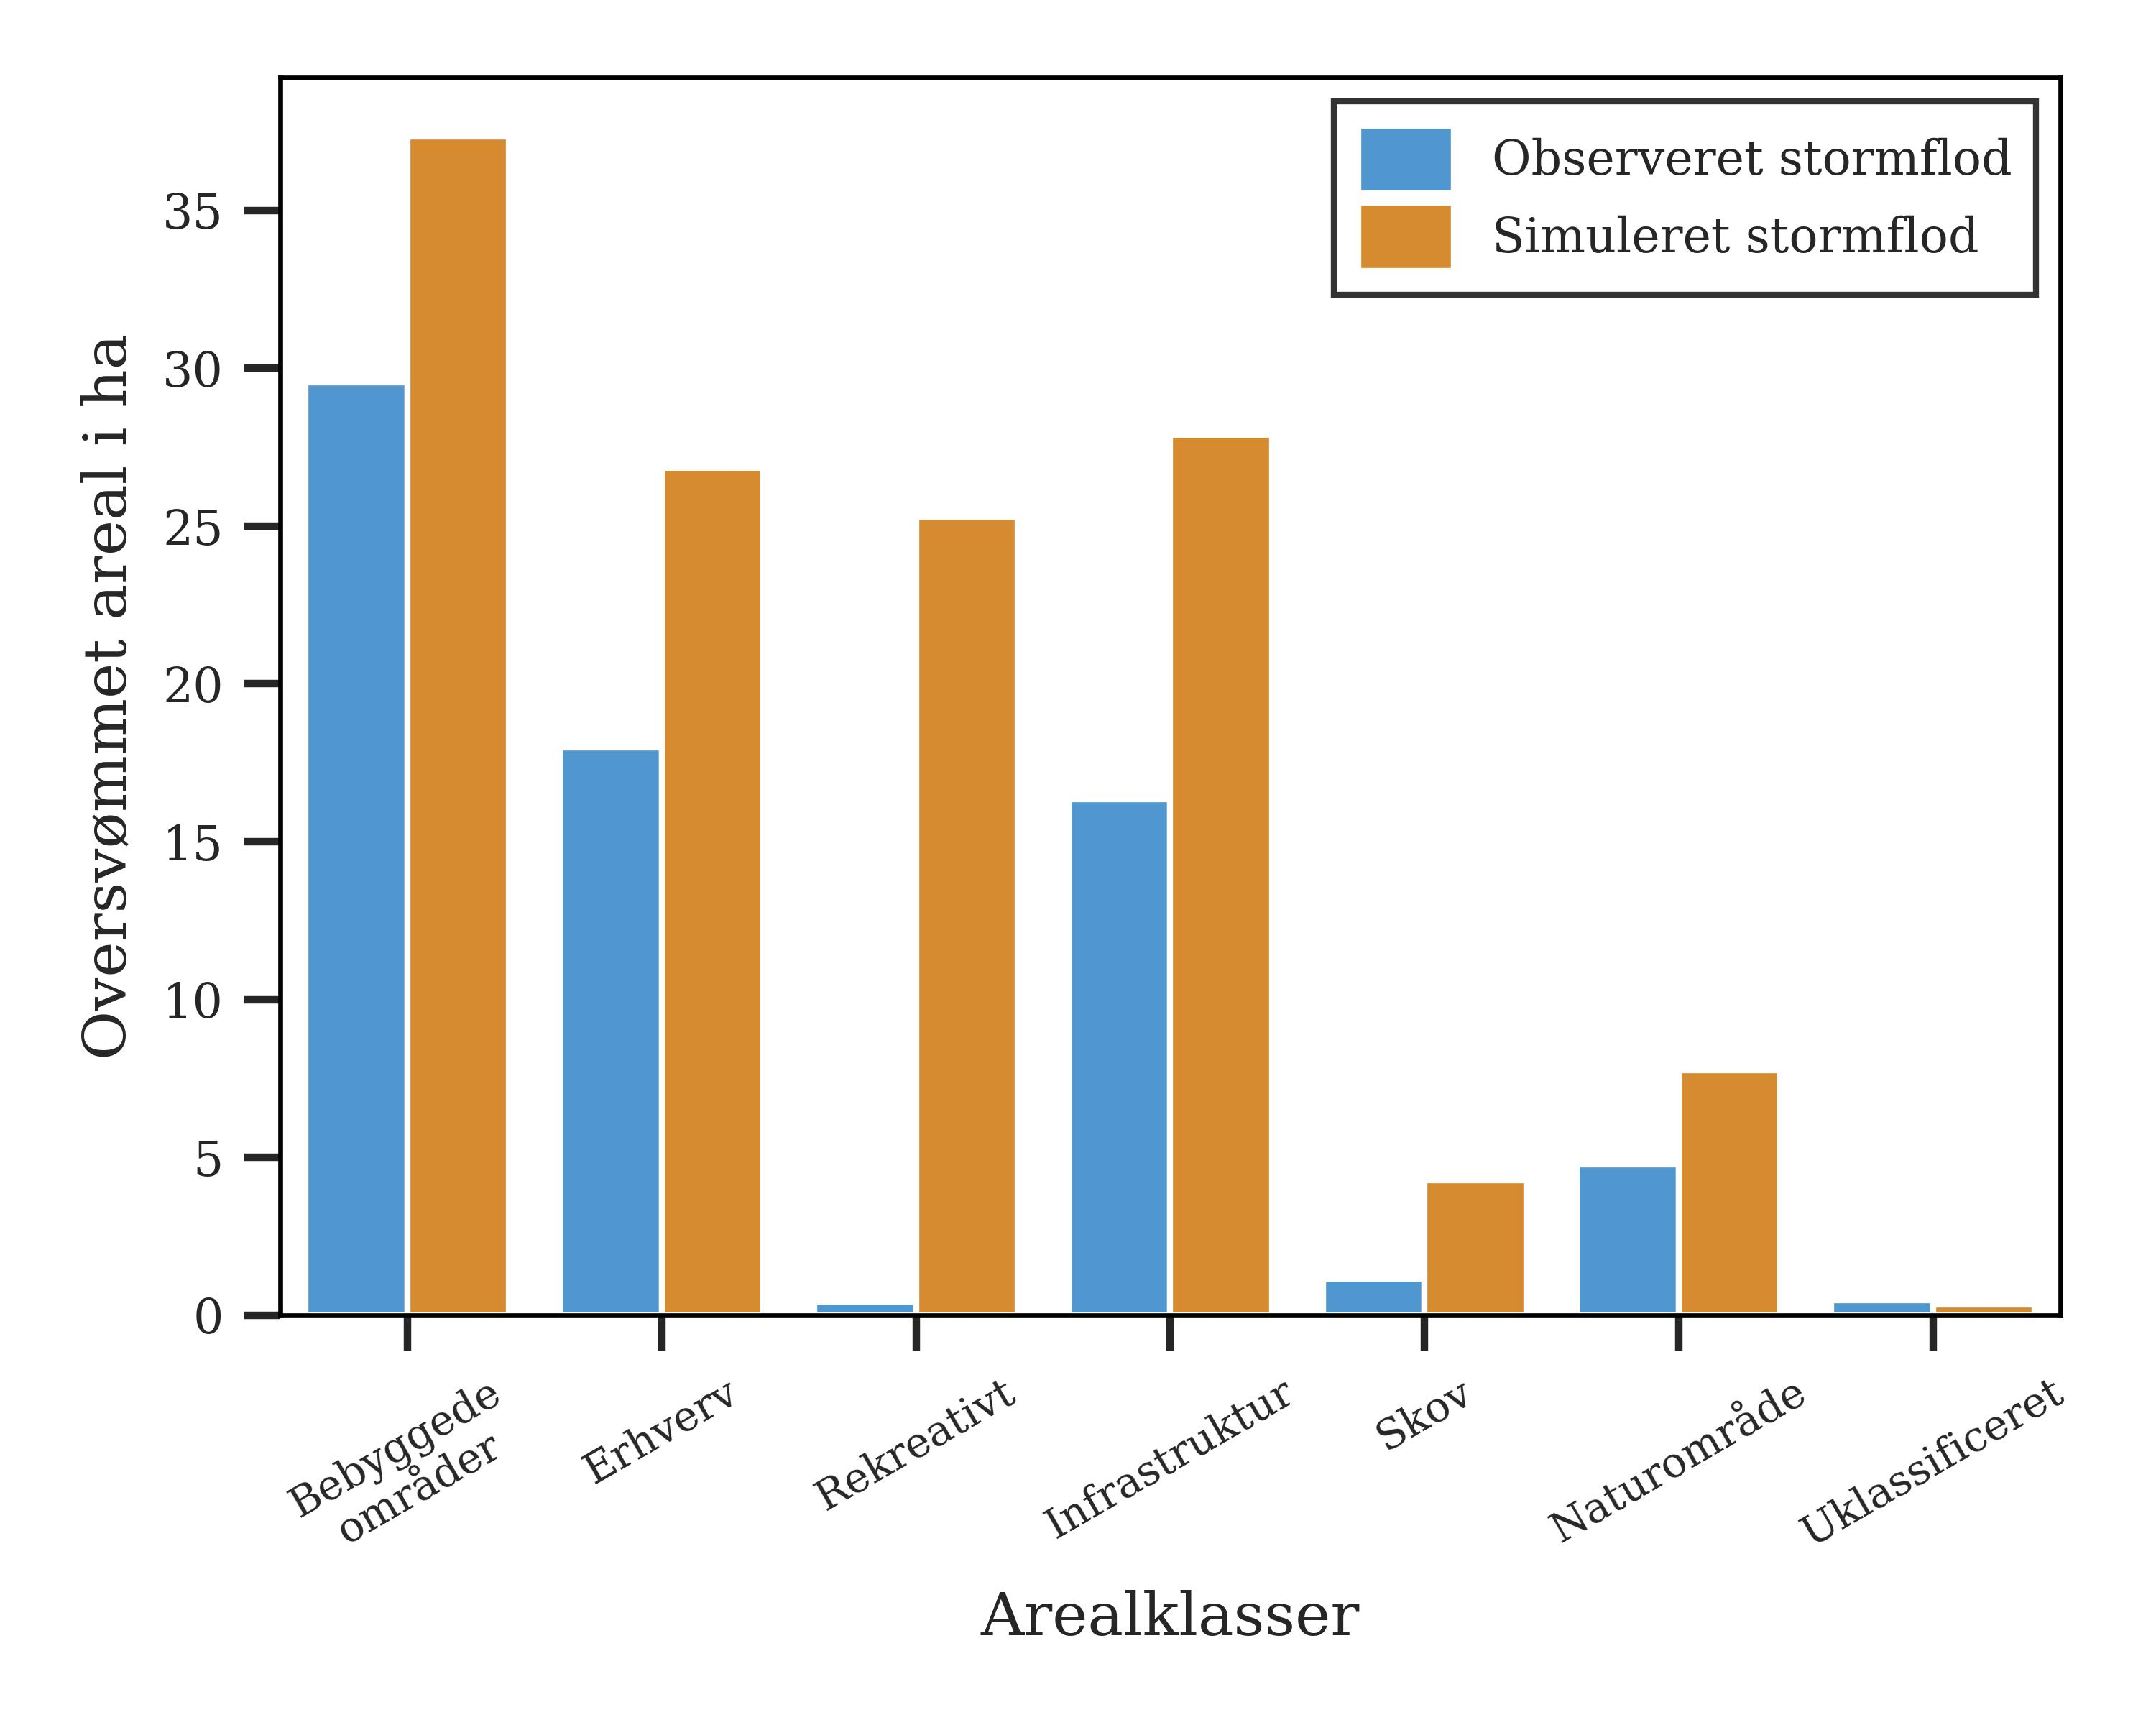
\includegraphics[width=1\linewidth]{images/Resultater/areal_anvendelses_grafer/aabenraa_oversvommet_Hektar.jpg}
        \caption{}
        \label{Subfig: Hektar arealklasser Aabenraa}
    \end{subfigure}
    \caption{Påvirkede arealanvendelsesklasser i Aabenraa for den observeret og simuleret stormflod. \textbf{(a)} Oversømmet areal som procent af det totale areal. \textbf{(b)} Oversvømmet areal i hektar.}
    \label{Figur: Påvirket arealanvendelse Aabenraa}
\end{figure}

På figur \ref{Subfig: Målt Gedser} ses arealet af den observeret oversvømmelse af Gedser Havn af stormfloden. På figur \ref{Subfig: Model Gedser} er det simulerede resultat. Resultatet fra Inundation Modellen er ens med den observeret hændelse. Den observeret hændelse havde et oversvømmet areal på 34,5 ha kontra 33,2 ha fra Inundation Modellen. Modellens resultat er dermed ca. 4\% mindre, svarende til ca. 1,3 ha. Det er primært arealet omkring lystbådehavnen nord for færgehavnen og et lavliggende naturområde vest for færgehavnen der blev oversvømmet. Dette fremgår af både det observeret data og den simuleret hændelse.   
\begin{figure}[H]
    \begin{subfigure}[t]{0.5\textwidth}
        \centering
        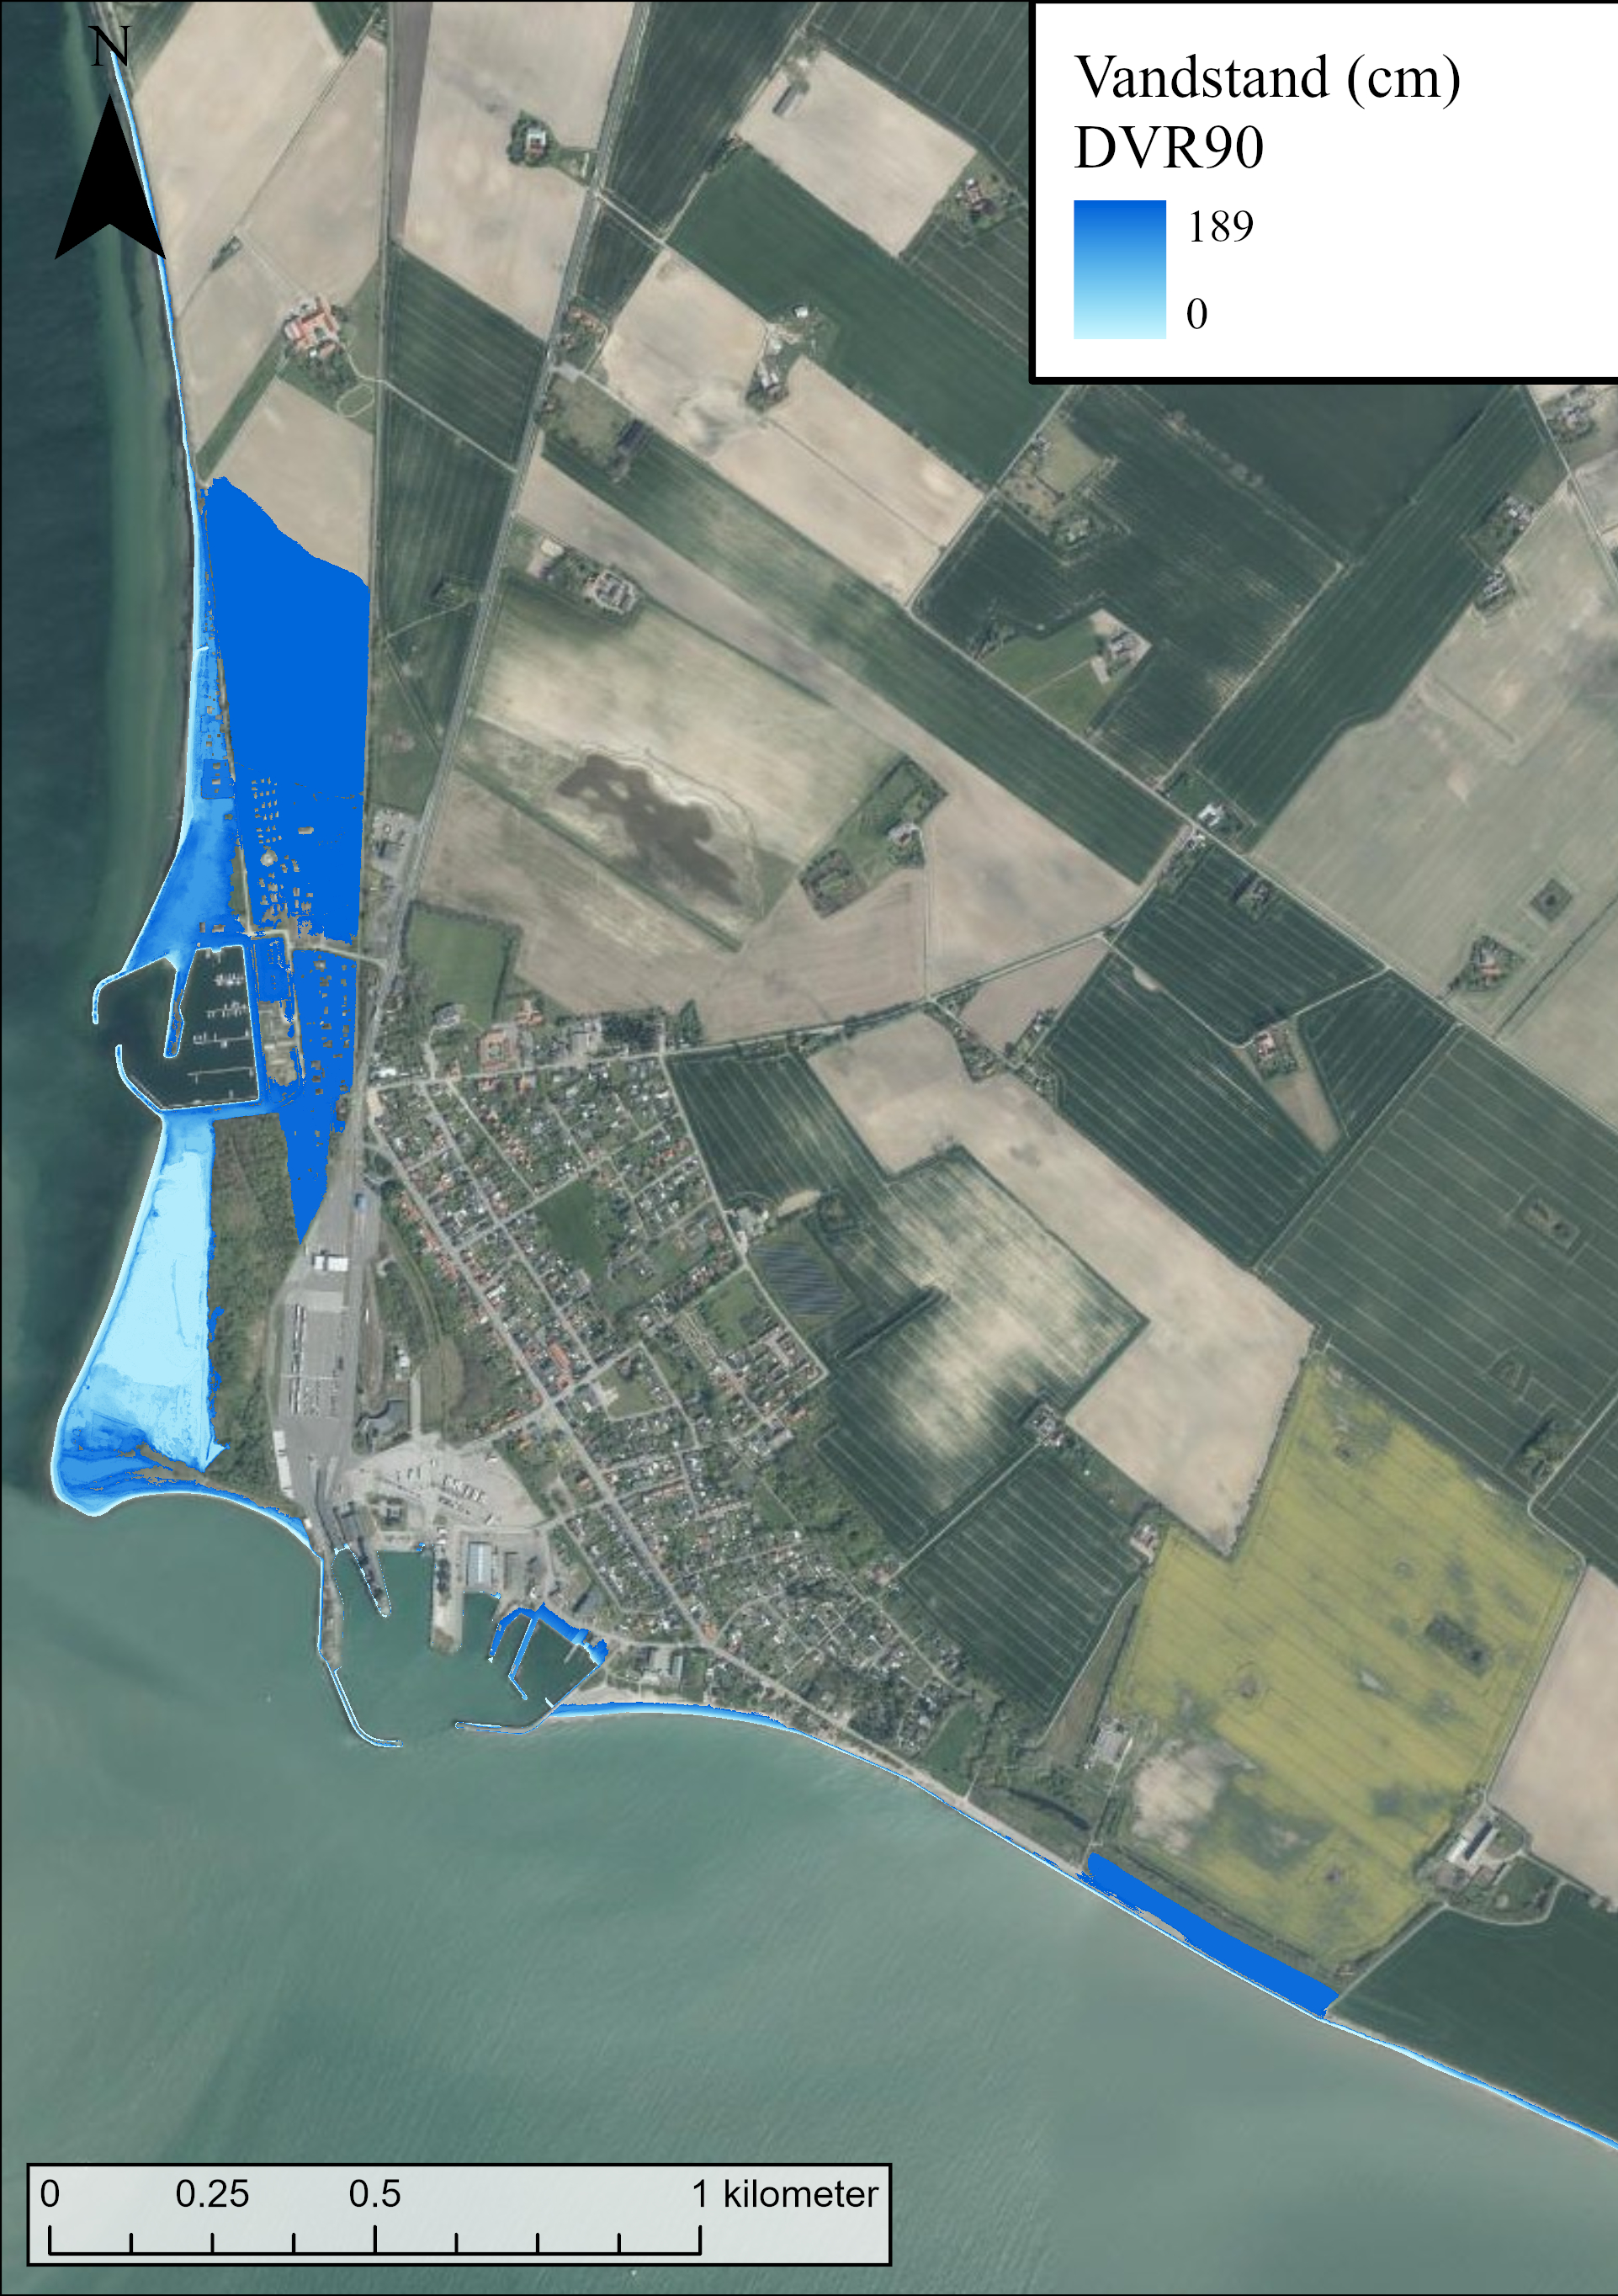
\includegraphics[width=0.95\linewidth]{images/Resultater/2023Malt/2023 resultat_gedser.jpg}
        \caption{}
        \label{Subfig: Målt Gedser}
    \end{subfigure}
    \begin{subfigure}[t]{0.5\textwidth}
        \centering
        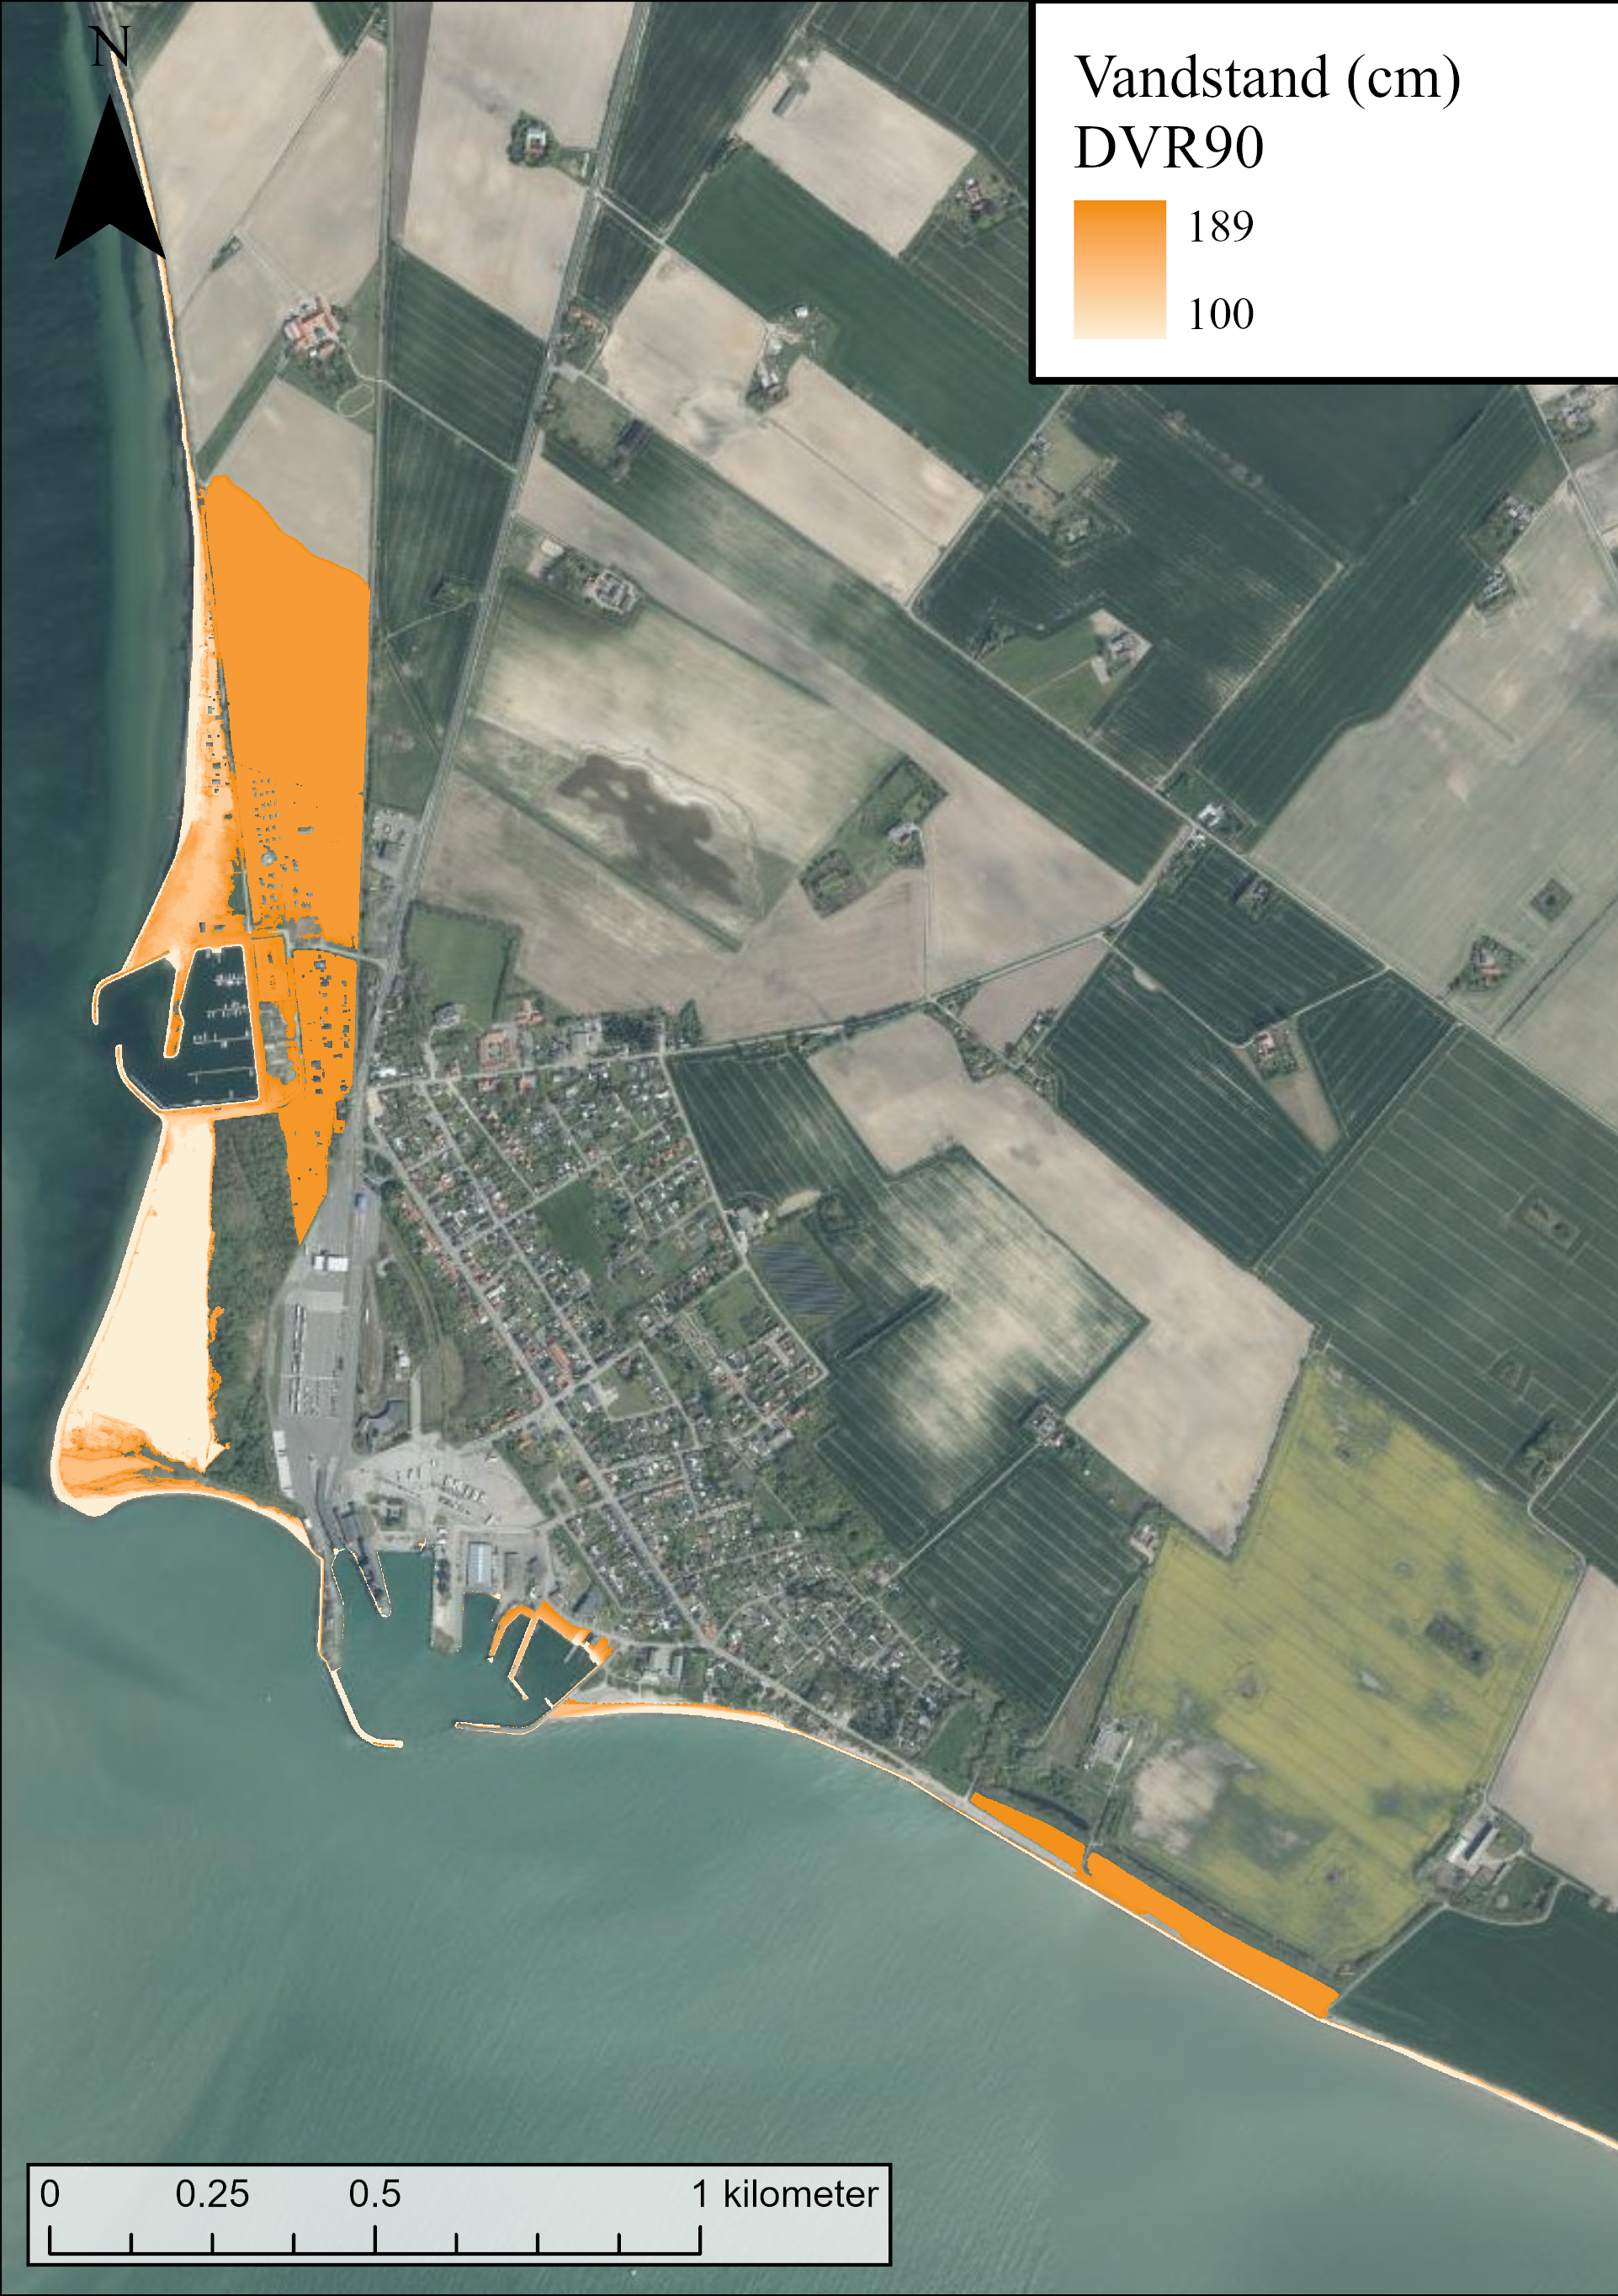
\includegraphics[width=0.95\linewidth]{images/Resultater/2023Model/2023 model_gedser.jpg}
        \caption{}
        \label{Subfig: Model Gedser}
    \end{subfigure}
    \caption{Oversvømmelseskort over 2023-stormfloden for Gedser Havn. \textbf{(a)} Observeret data. \textbf{(b)} Simuleret data}
    \label{Figur: Målt & simuleret Gedser}
\end{figure}

I Gedser Havn blev otte arealklasser påvirket af oversvømmelserne under stormfloden. Ved både den observeret og simuleret stormflod er det naturområder der blev mest påvirket med 17,7 og 17,2 ha, svarende til henholdsvis 51,5 og 51,7\% af det samlet areal (figur \ref{Subfig: Procent areal Gedser} og \ref{Subfig: Hektar areal Gedser}).
Andelen og arealet af de andre oversvømmet arealer er ens for begge resultater (figur \ref{Figur: Påvirket arealanvendelse Gedser}).
\begin{figure}[H]
    \begin{subfigure}[b]{0.5\textwidth}
        \centering
        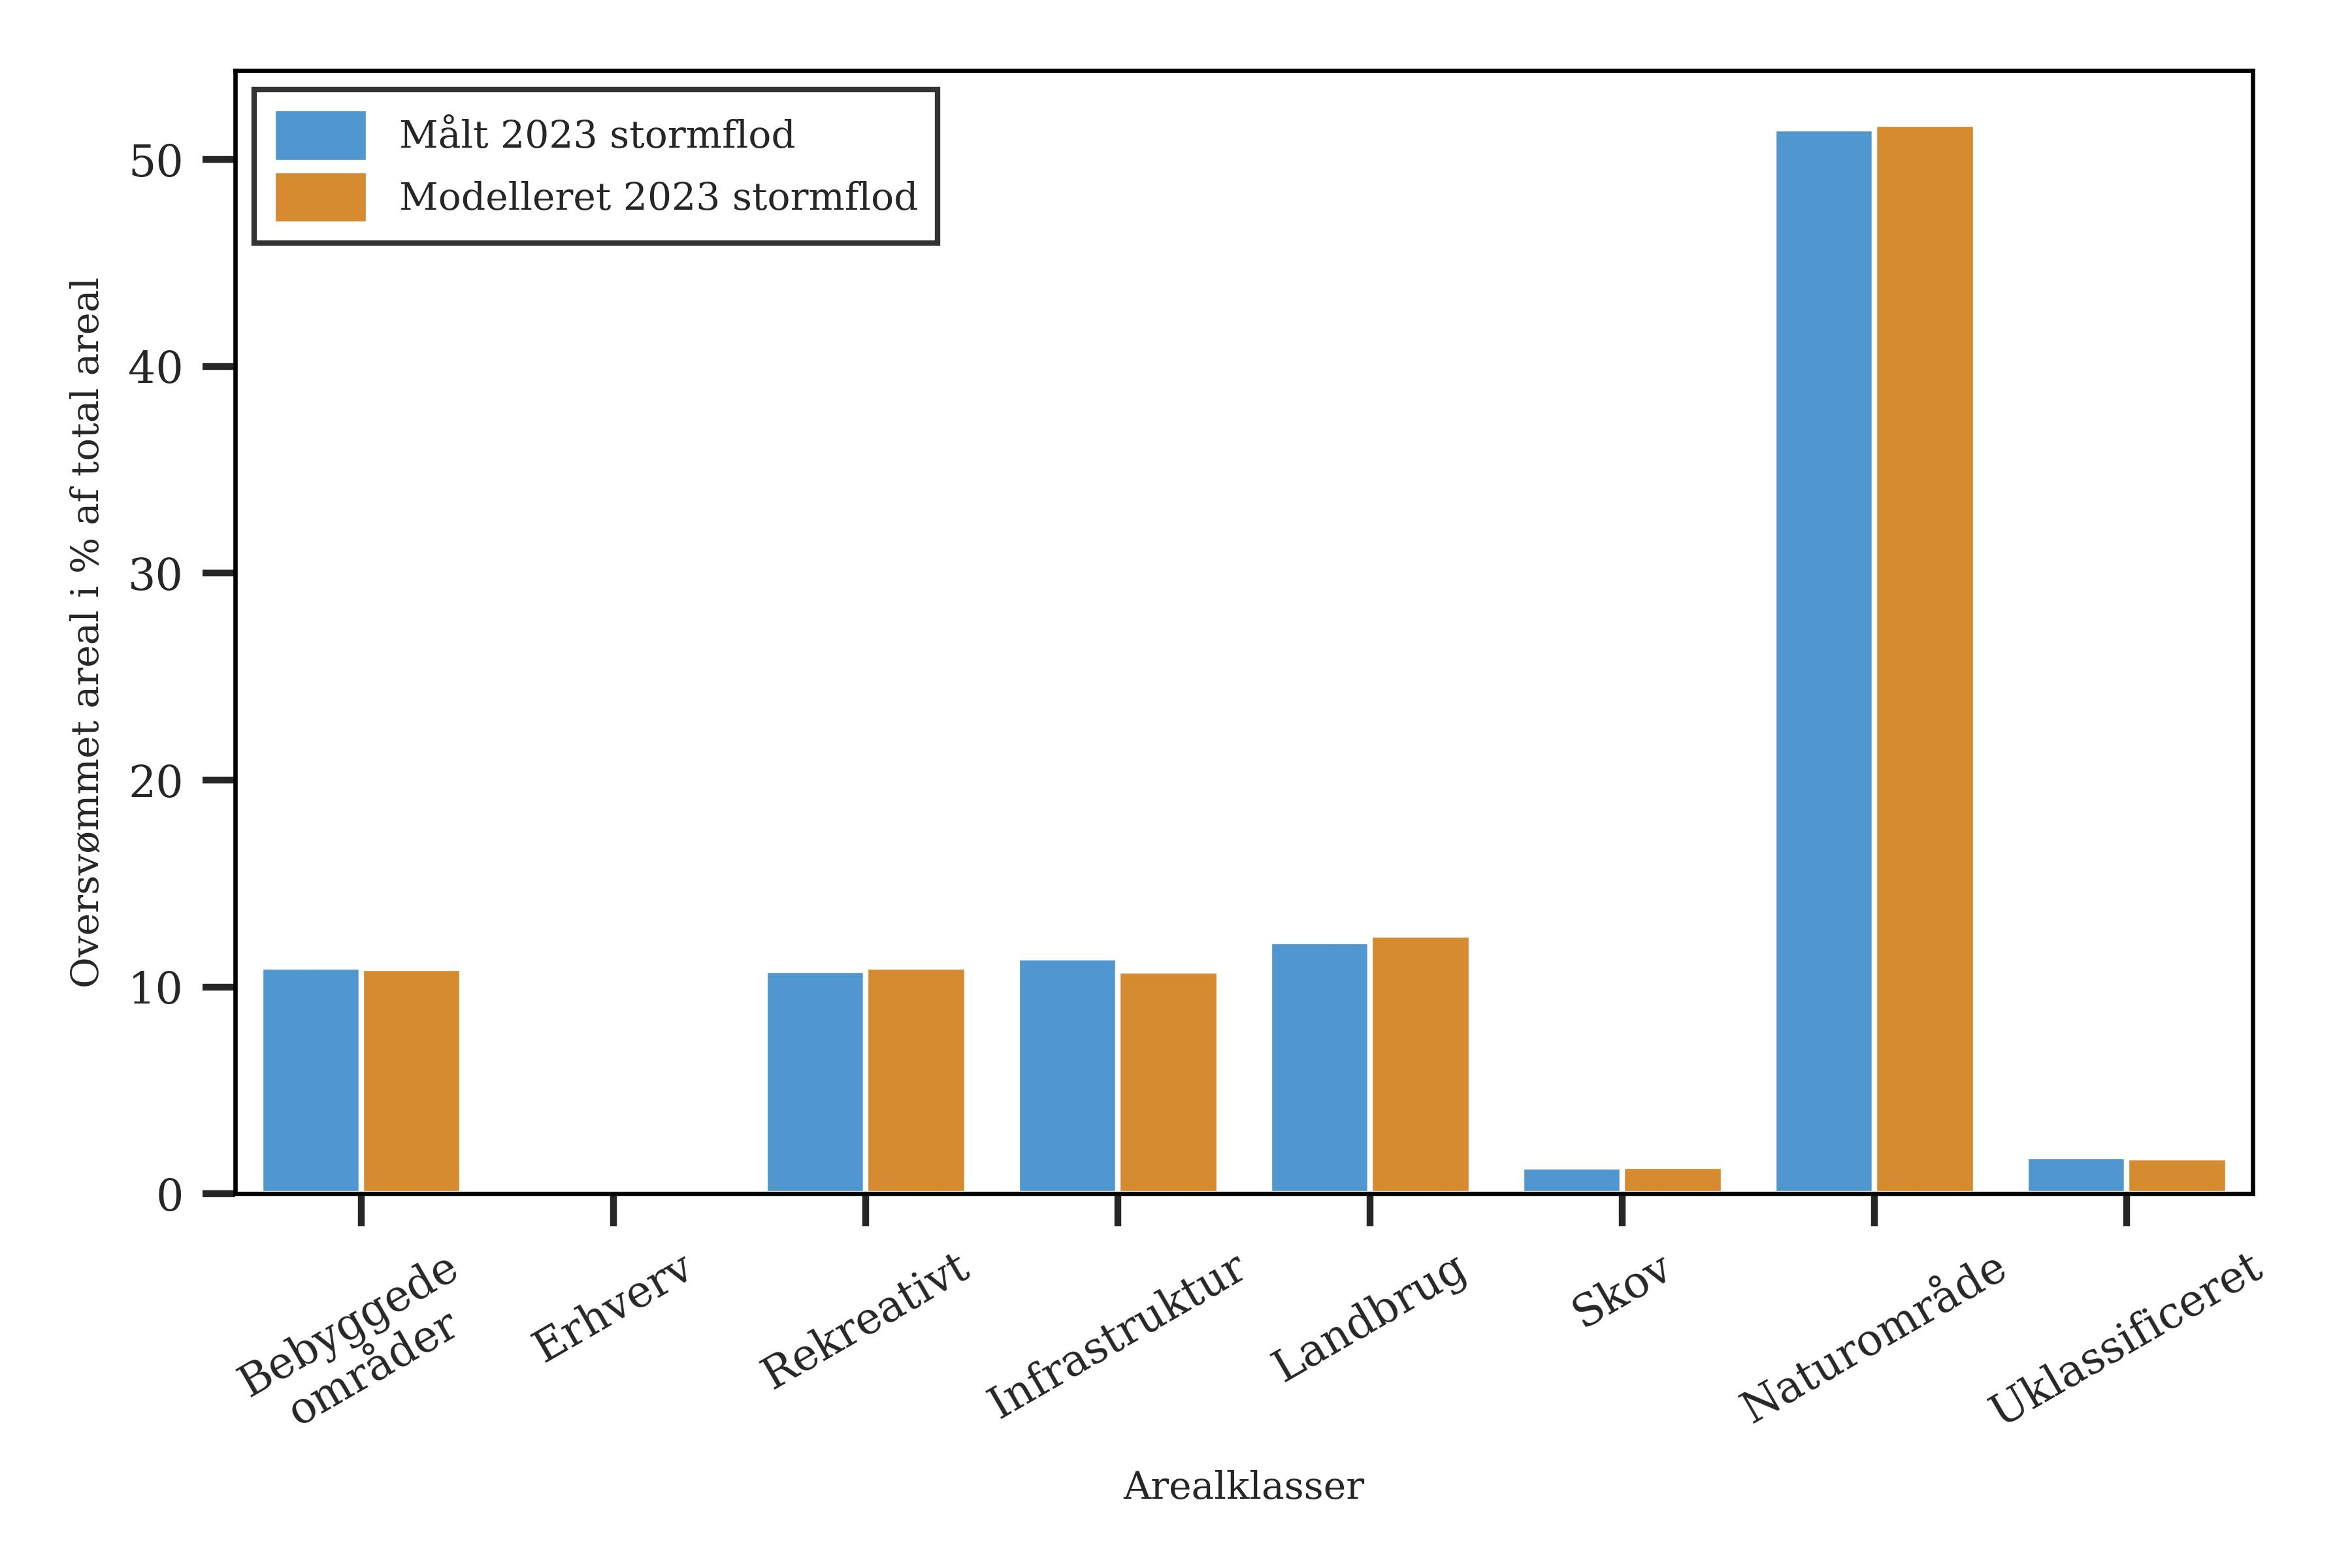
\includegraphics[width=1\linewidth]{images/Resultater/areal_anvendelses_grafer/gedser_arealanvendelse.jpg}
        \caption{}
        \label{Subfig: Procent areal Gedser}
    \end{subfigure}
    \begin{subfigure}[b]{0.5\textwidth}
        \centering
        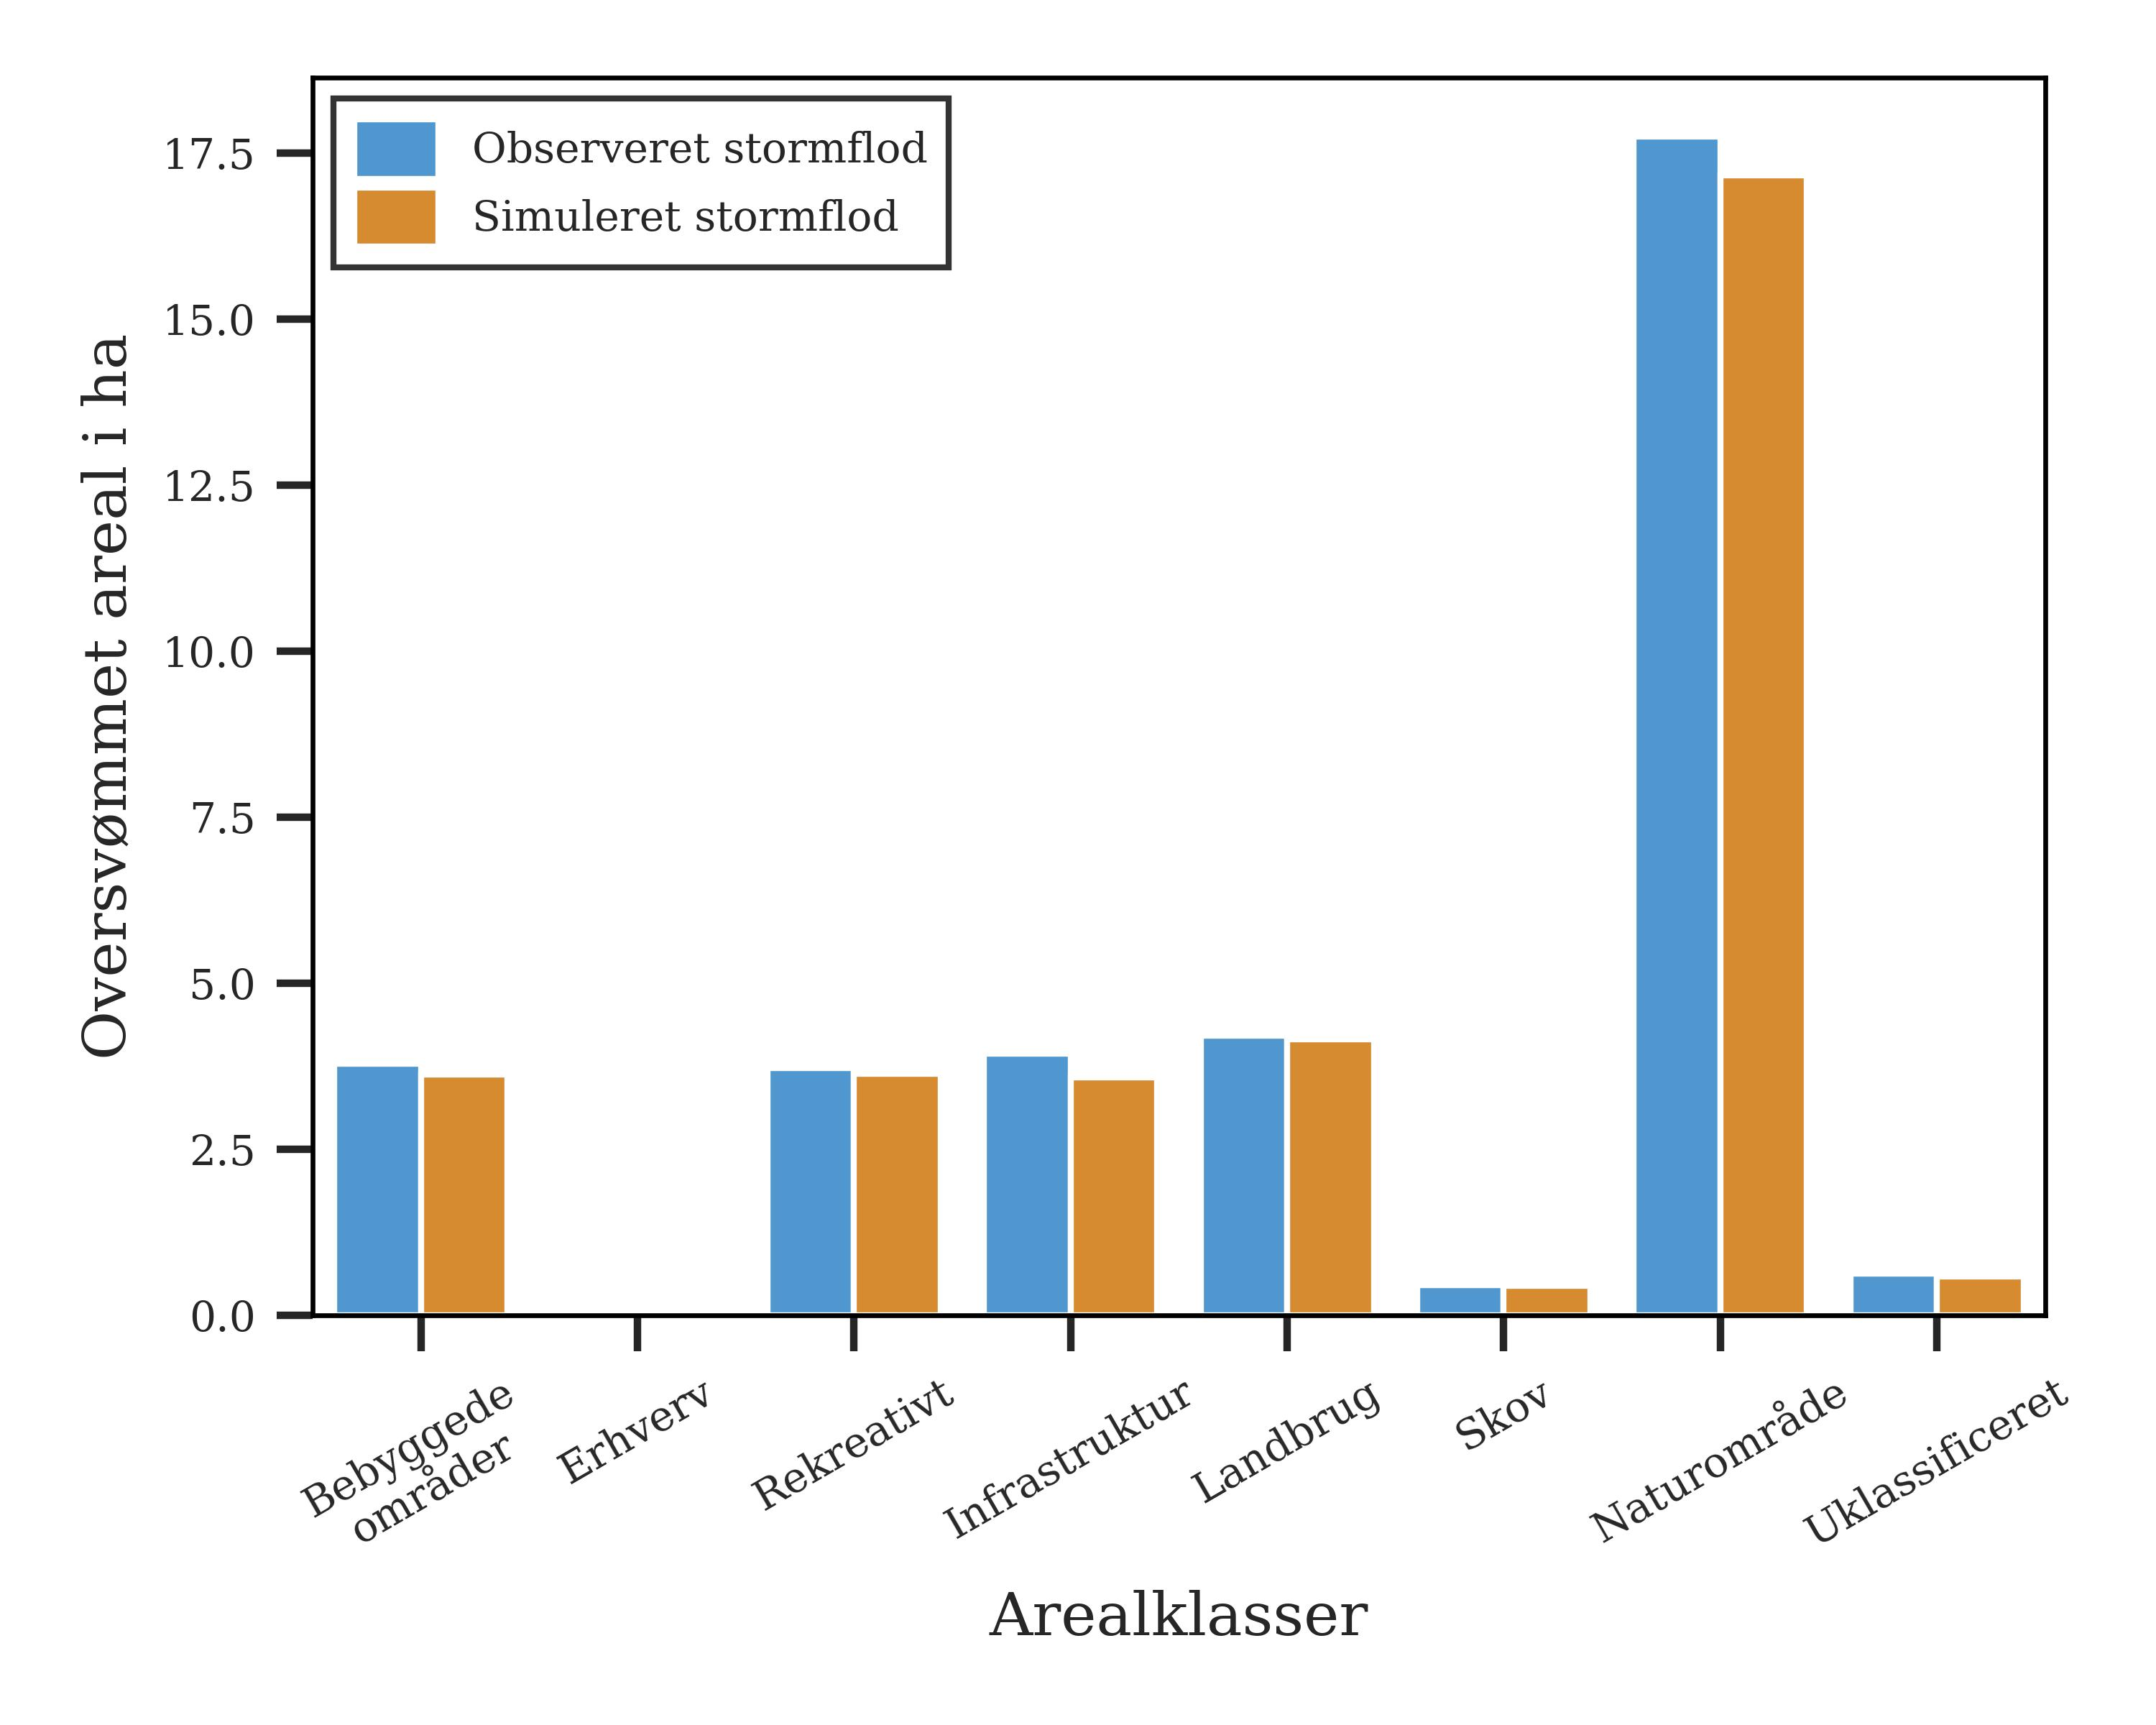
\includegraphics[width=1\linewidth]{images/Resultater/areal_anvendelses_grafer/gedser_oversvommet_Hektar.jpg}
        \caption{}
        \label{Subfig: Hektar areal Gedser}
    \end{subfigure}
    \caption{Påvirkede arealanvendelsesklasser i Gedser Havn for den observeret og simuleret stormflod. Bemærk at kategorien "Erhverv" \hspace{0.1cm}udgør >0,05\% og er derfor ikke synlig. \textbf{(a)} Oversømmet areal som procent af det totale areal. \textbf{(b)} Oversvømmet areal i hektar.}
    \label{Figur: Påvirket arealanvendelse Gedser}
\end{figure}

For Hesnæs var det primært havnen, inklusiv havnens mole og kystlinjen der blev oversvømmet under stormfloden (figur \ref{Subfig: Målt Hesnæs}). Resultatet fra Inundation Modellen i figur \ref{Subfig: Model Hesnæs} giver det samme resultat og der er ikke forskel mellem det observeret og simuleret resultat. Den observeret hændelse havde et totalt oversvømmet areal på 34,6 ha og det simulerede resultat havde et areal på 33 ha. Modellens resultat er derfor 1,6 ha mindre, svarende til en forskel på 5,2\%.
\begin{figure}[H]
    \begin{subfigure}[t]{0.5\textwidth}
        \centering
        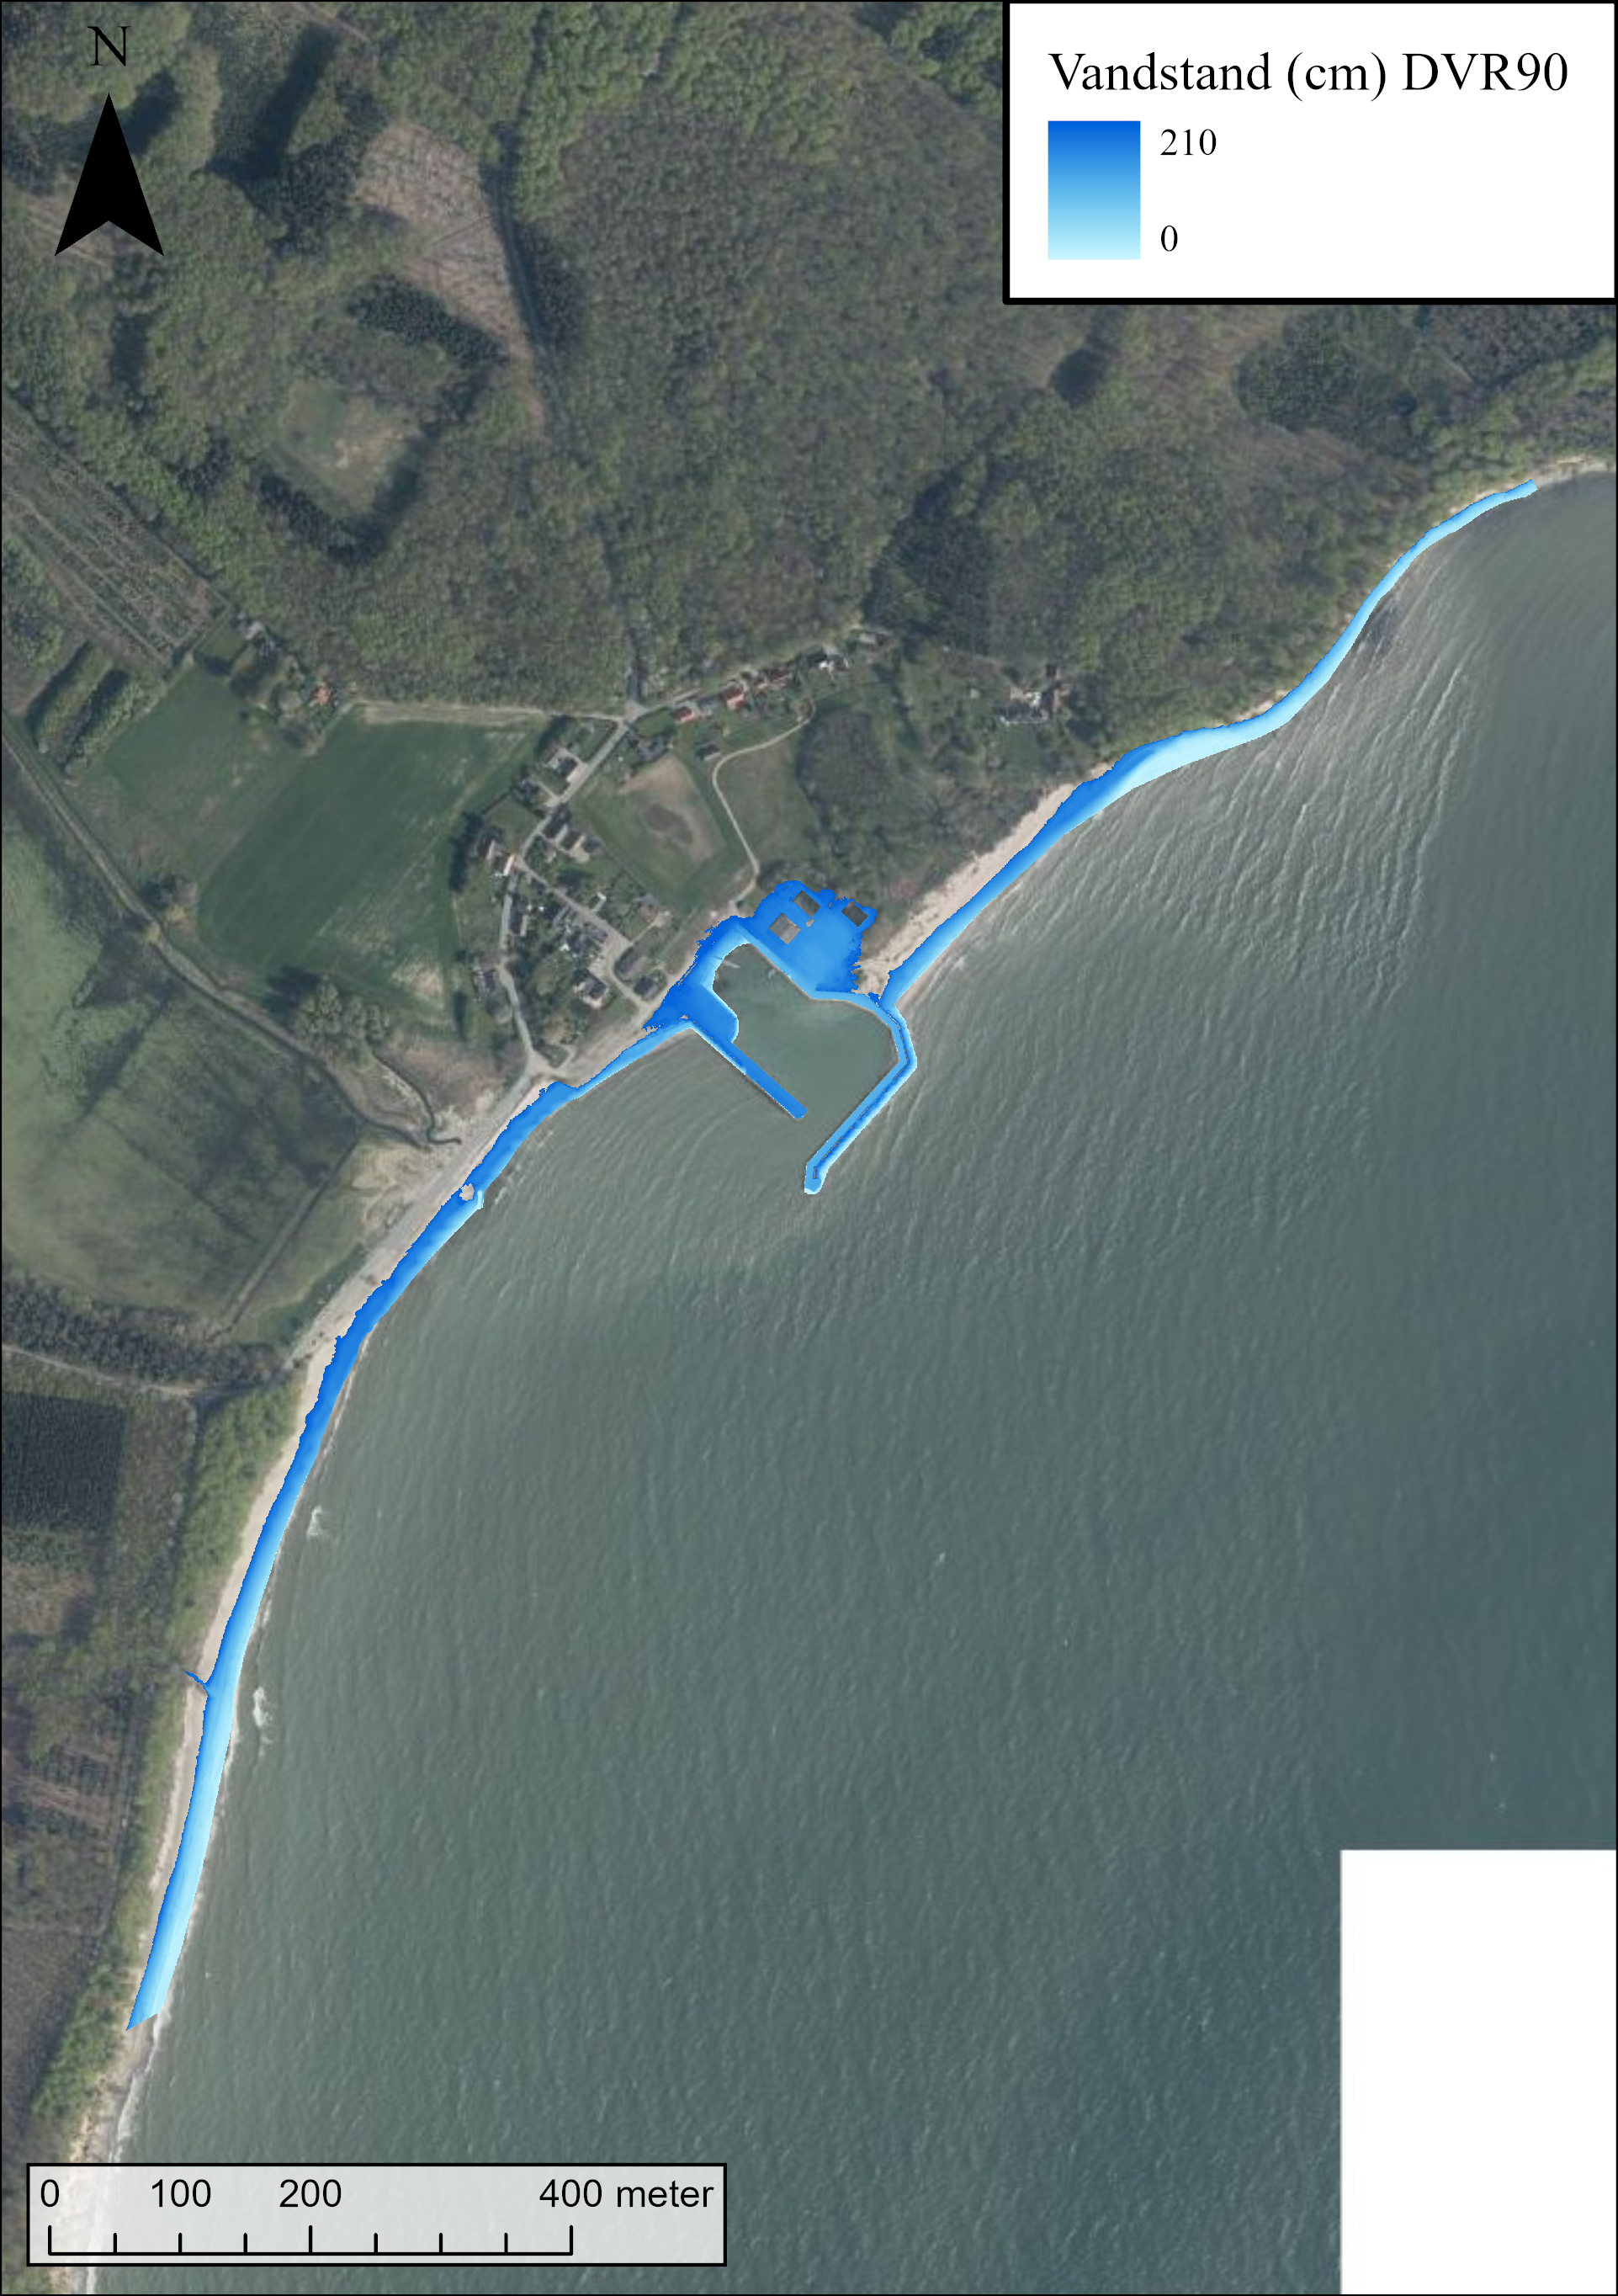
\includegraphics[width=0.95\linewidth]{images/Resultater/2023Malt/2023 resultat_hesnaes.jpg}
        \caption{}
        \label{Subfig: Målt Hesnæs}
    \end{subfigure}
    \begin{subfigure}[t]{0.5\textwidth}
        \centering
        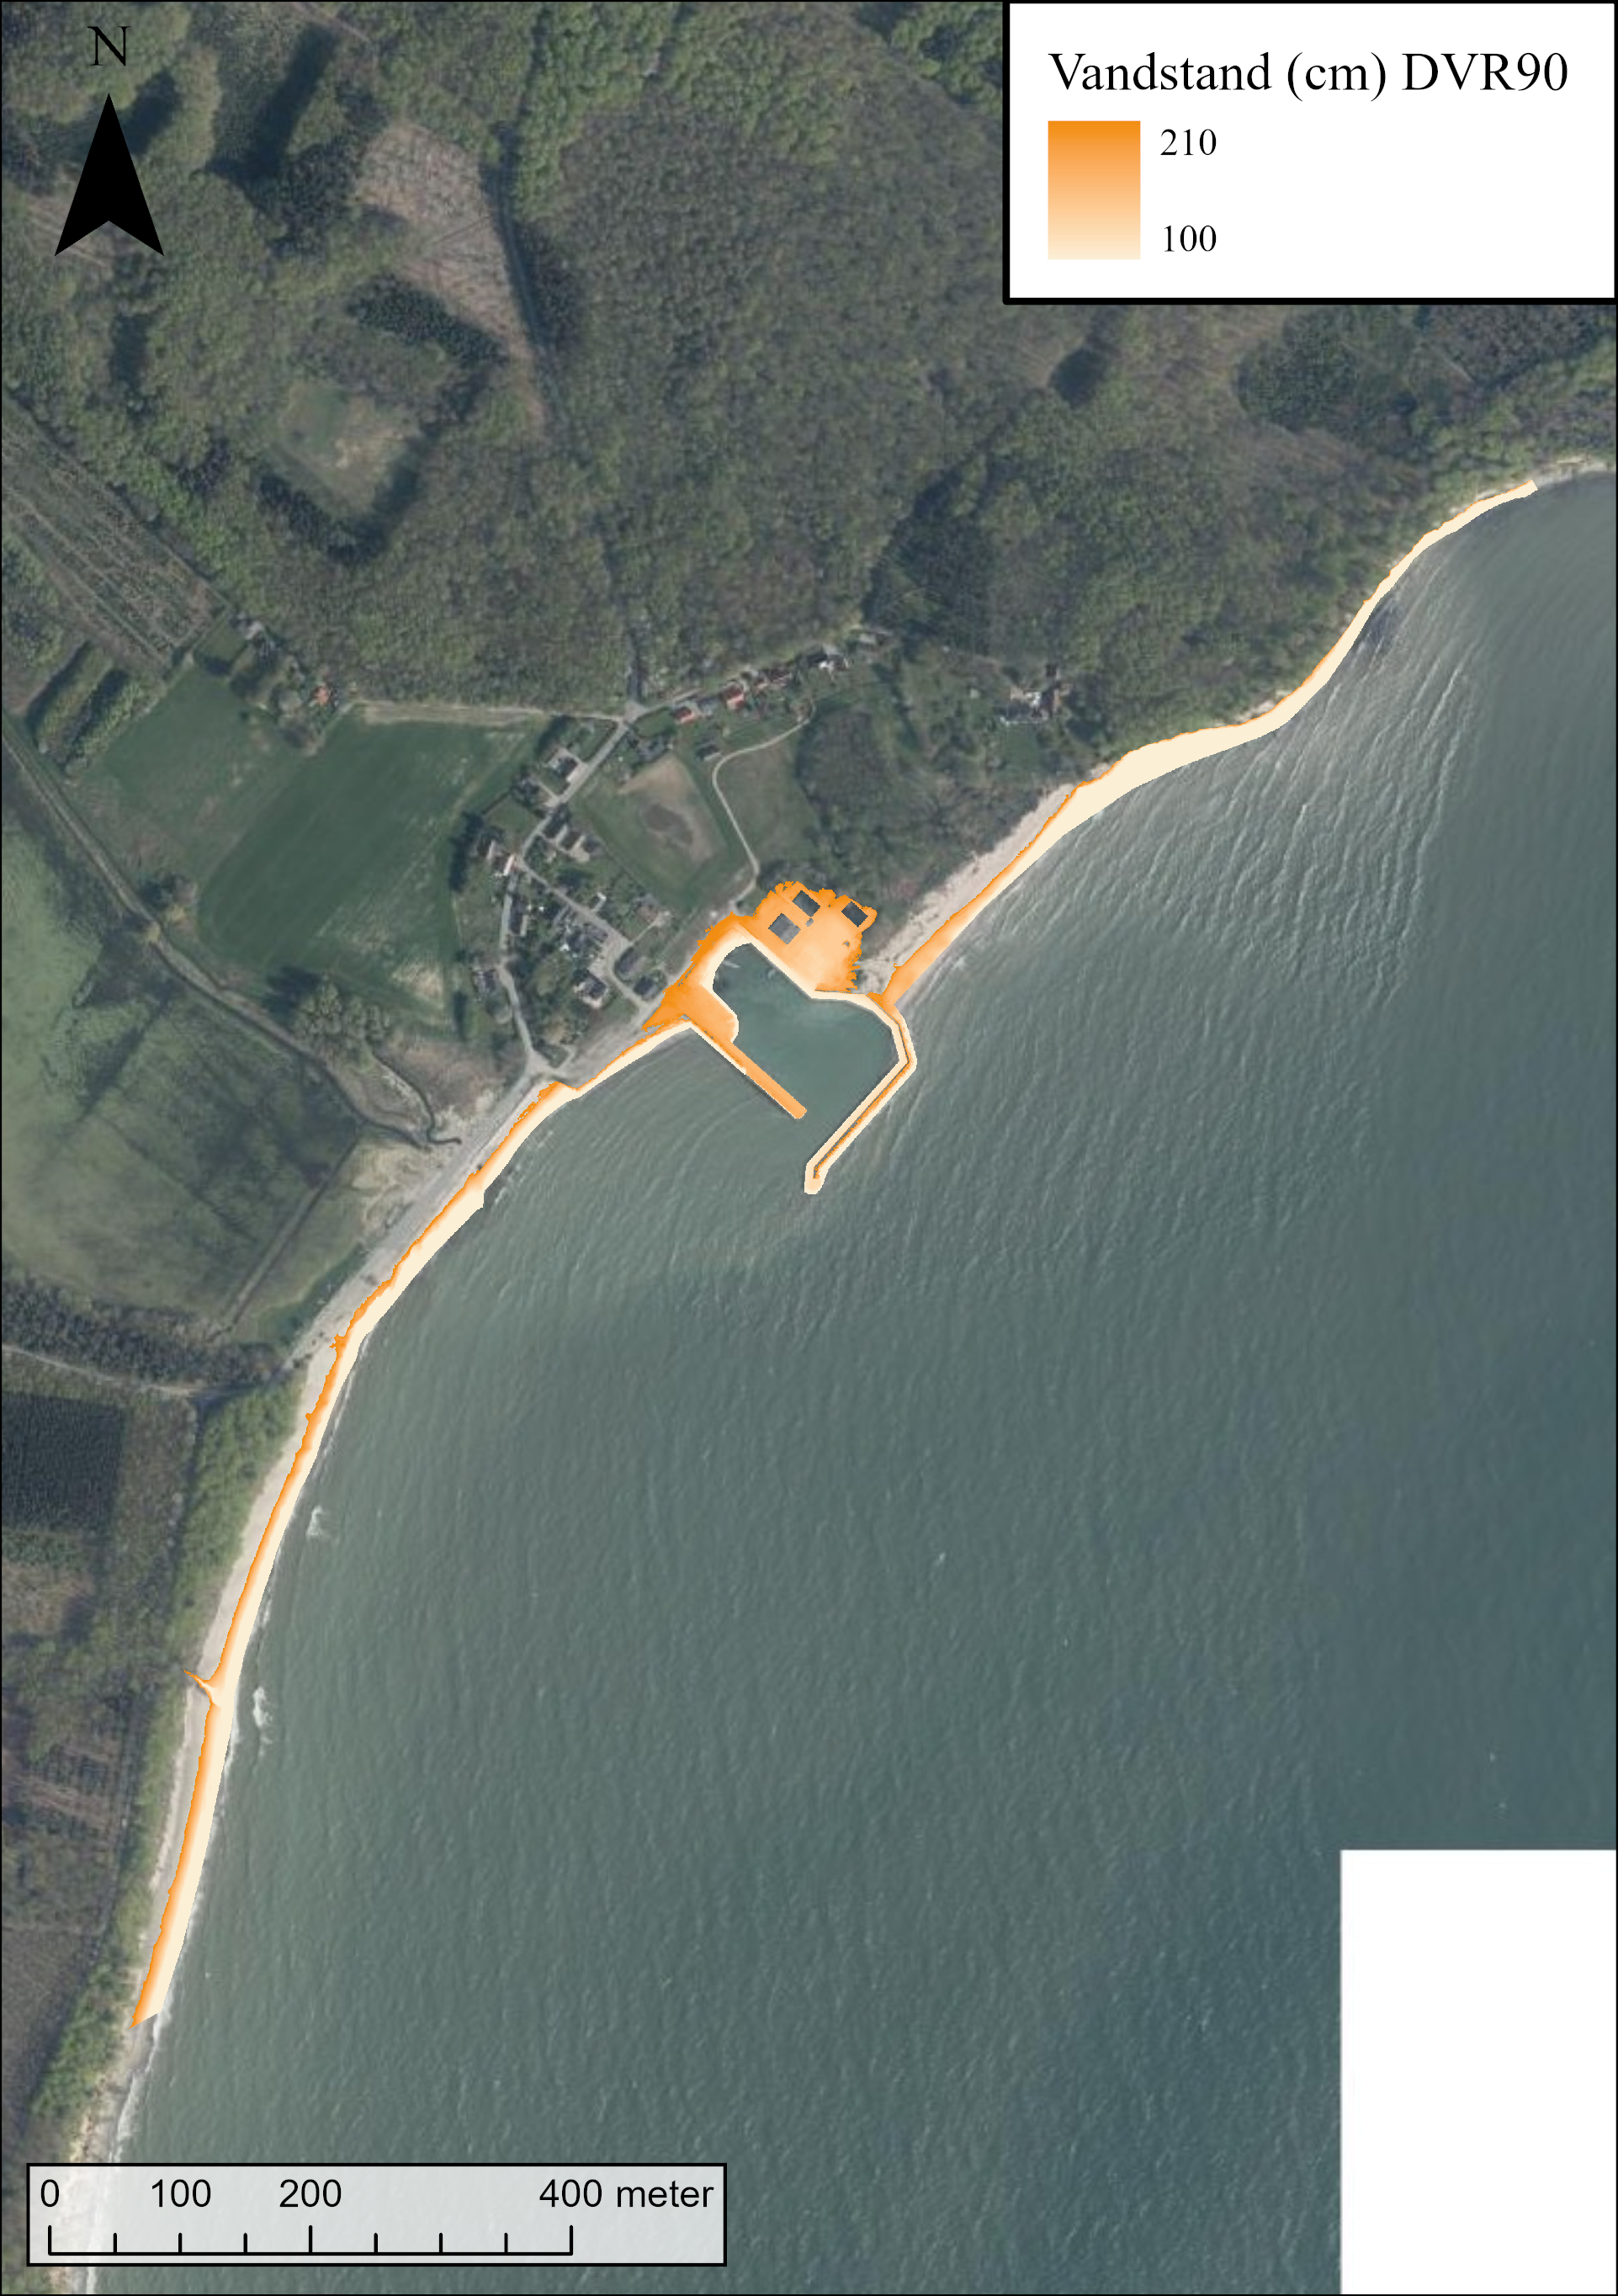
\includegraphics[width=0.95\linewidth]{images/Resultater/2023Model/2023 model_hesnaes.jpg}
        \caption{}
        \label{Subfig: Model Hesnæs}
    \end{subfigure}
    \caption{Oversvømmelseskort over 2023-stormfloden for Hesnæs. \textbf{(a)} Observeret data. \textbf{(b)} Simuleret data.}
    \label{Figur: Målt & simuleret Hesnæs}
\end{figure} 

I Hesnæs blev seks forskellige arealanvendelser påvirket. De mest påvirkede arealer i Hesnæs var kysten, der falder ind under naturområder. Dette har været gældende for begge resultater. For den observeret hændelse blev 66,2\% naturområde oversvømmet og for den simuleret hændelse blev 65,8\% oversvømmet (figur \ref{Subfig: Procent hesnæs}). Dette svarer til henholdsvis 2,3 og 2,2 ha (figur \ref{Subfig: Hektar Hesnæs}). For de andre arealklasser er resultatet ens for den observeret og simuleret stormflod. 
\begin{figure}[H]
    \begin{subfigure}[b]{0.5\textwidth}
        \centering
        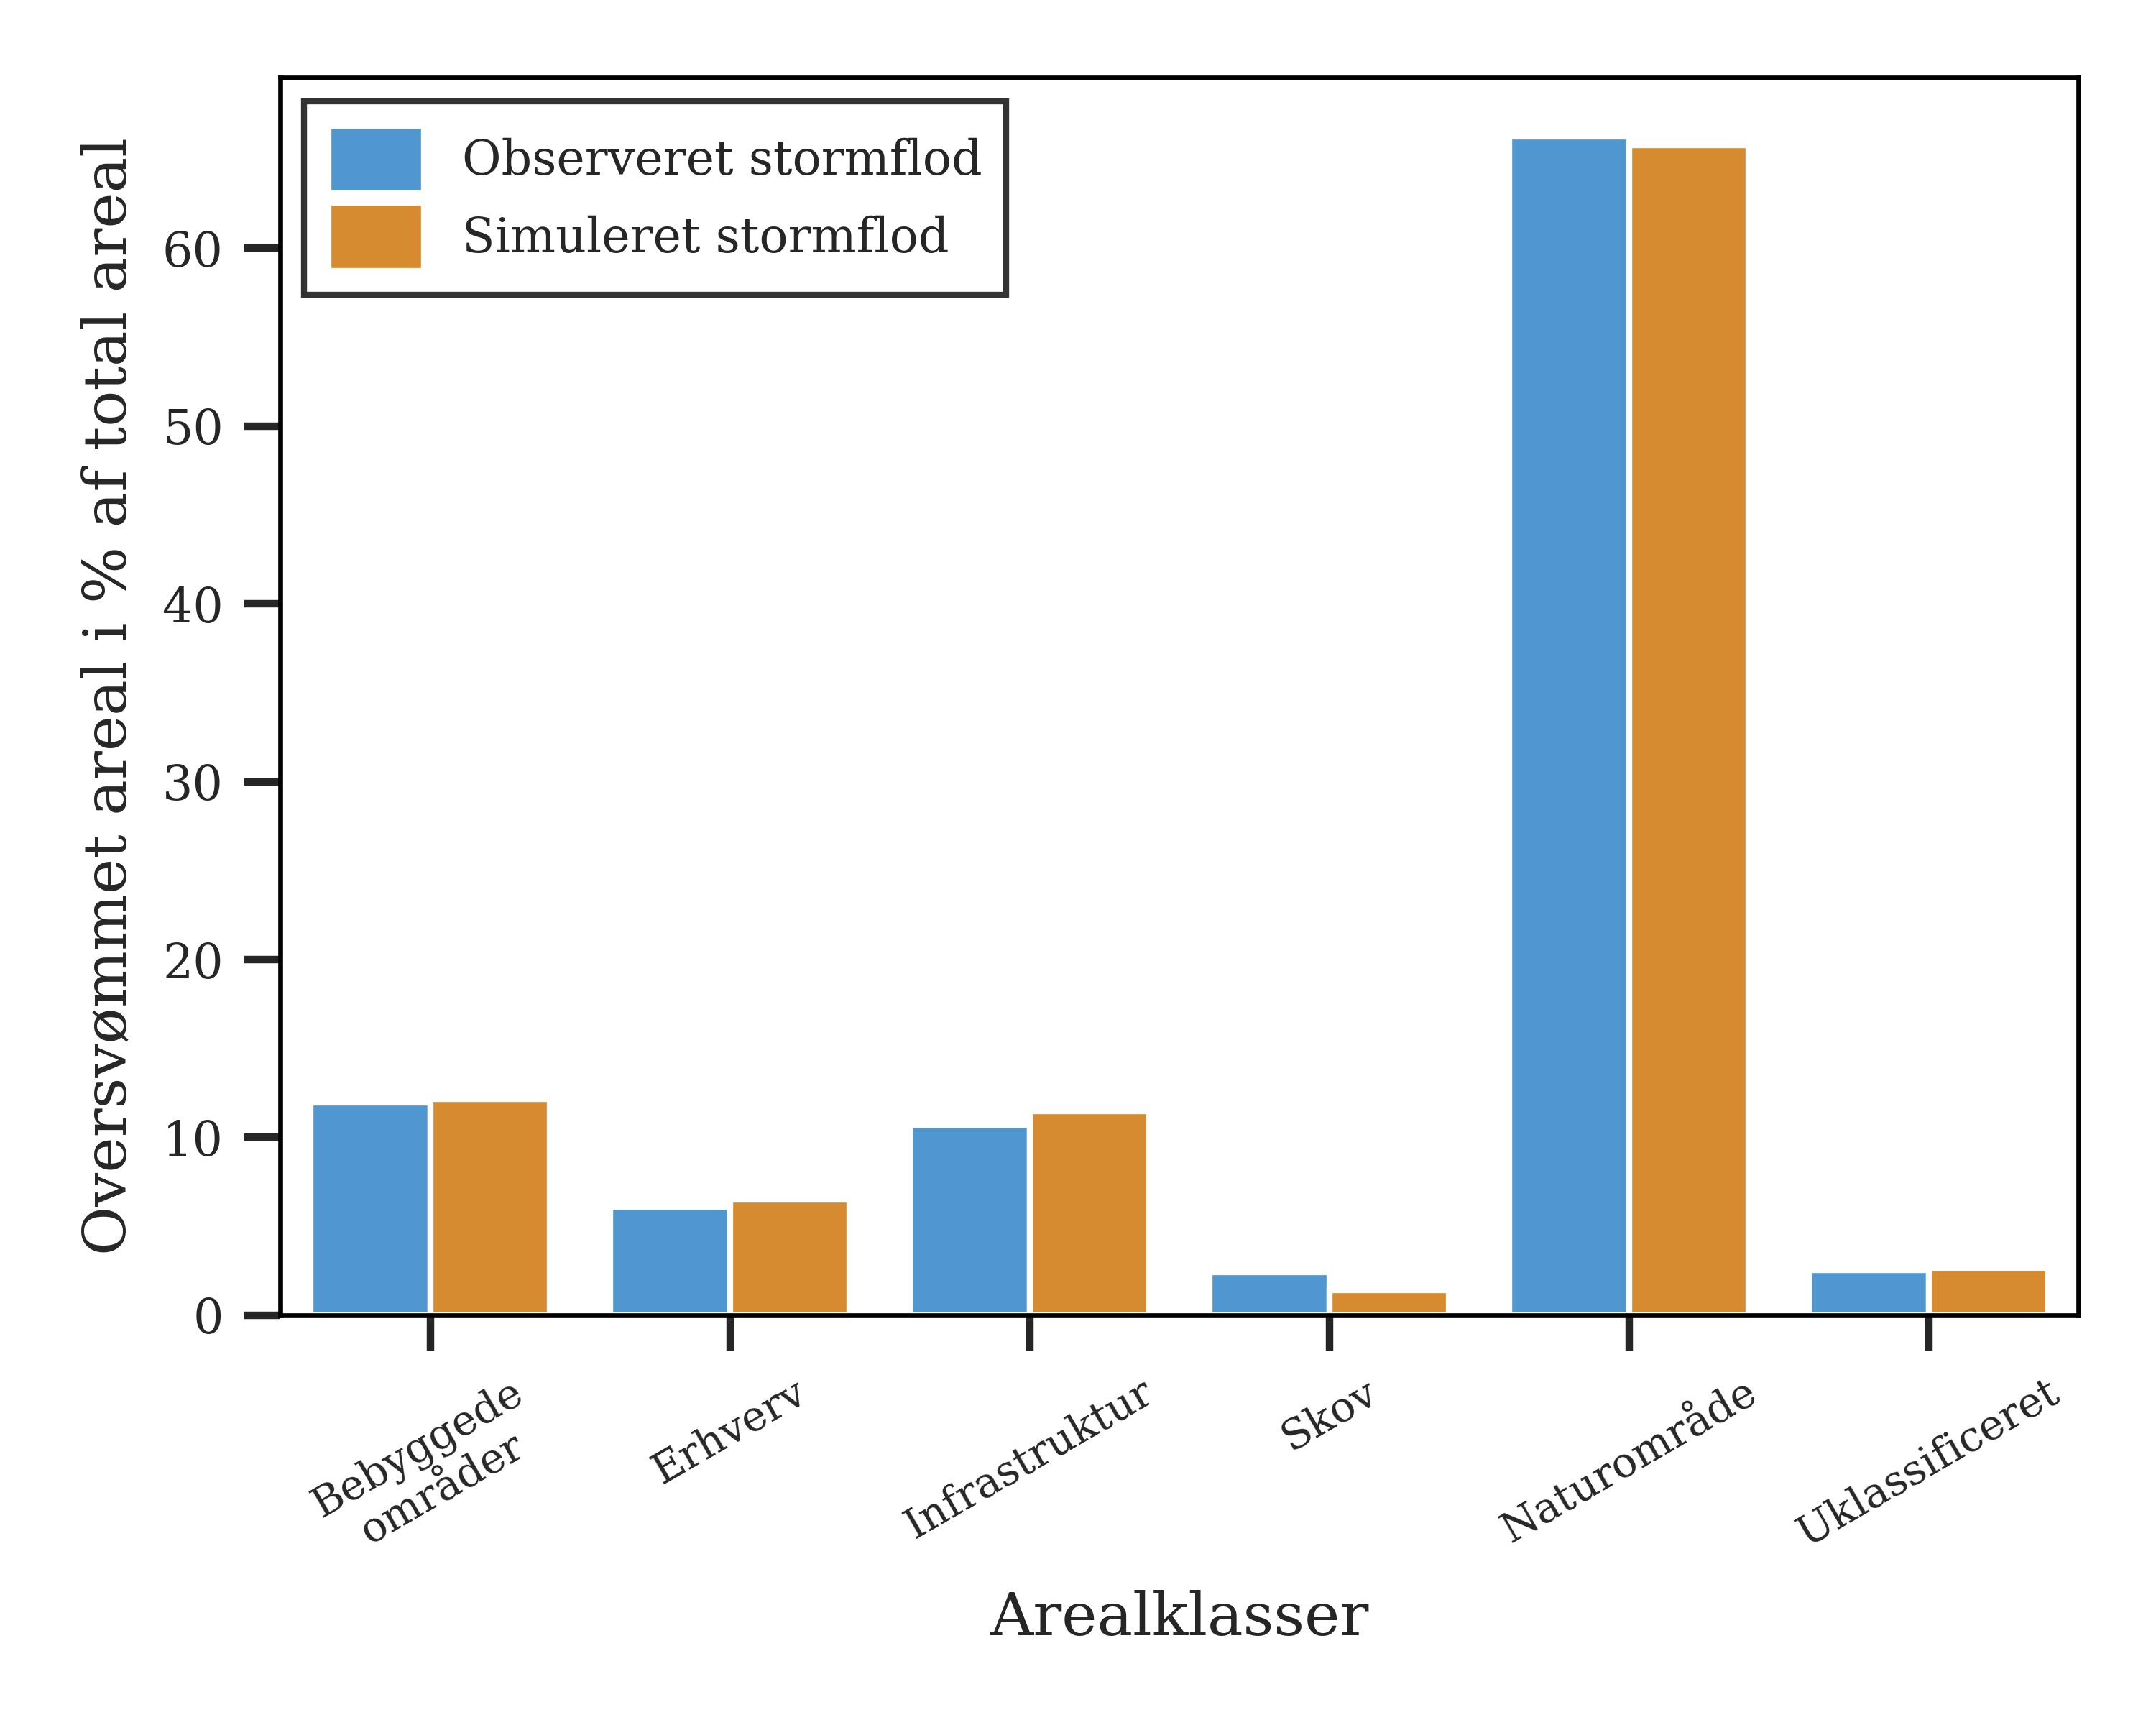
\includegraphics[width=1\linewidth]{images/Resultater/areal_anvendelses_grafer/hesnaes_arealanvendelse.jpg}
        \caption{}
        \label{Subfig: Procent hesnæs}
    \end{subfigure}
    \begin{subfigure}[b]{0.5\textwidth}
        \centering
        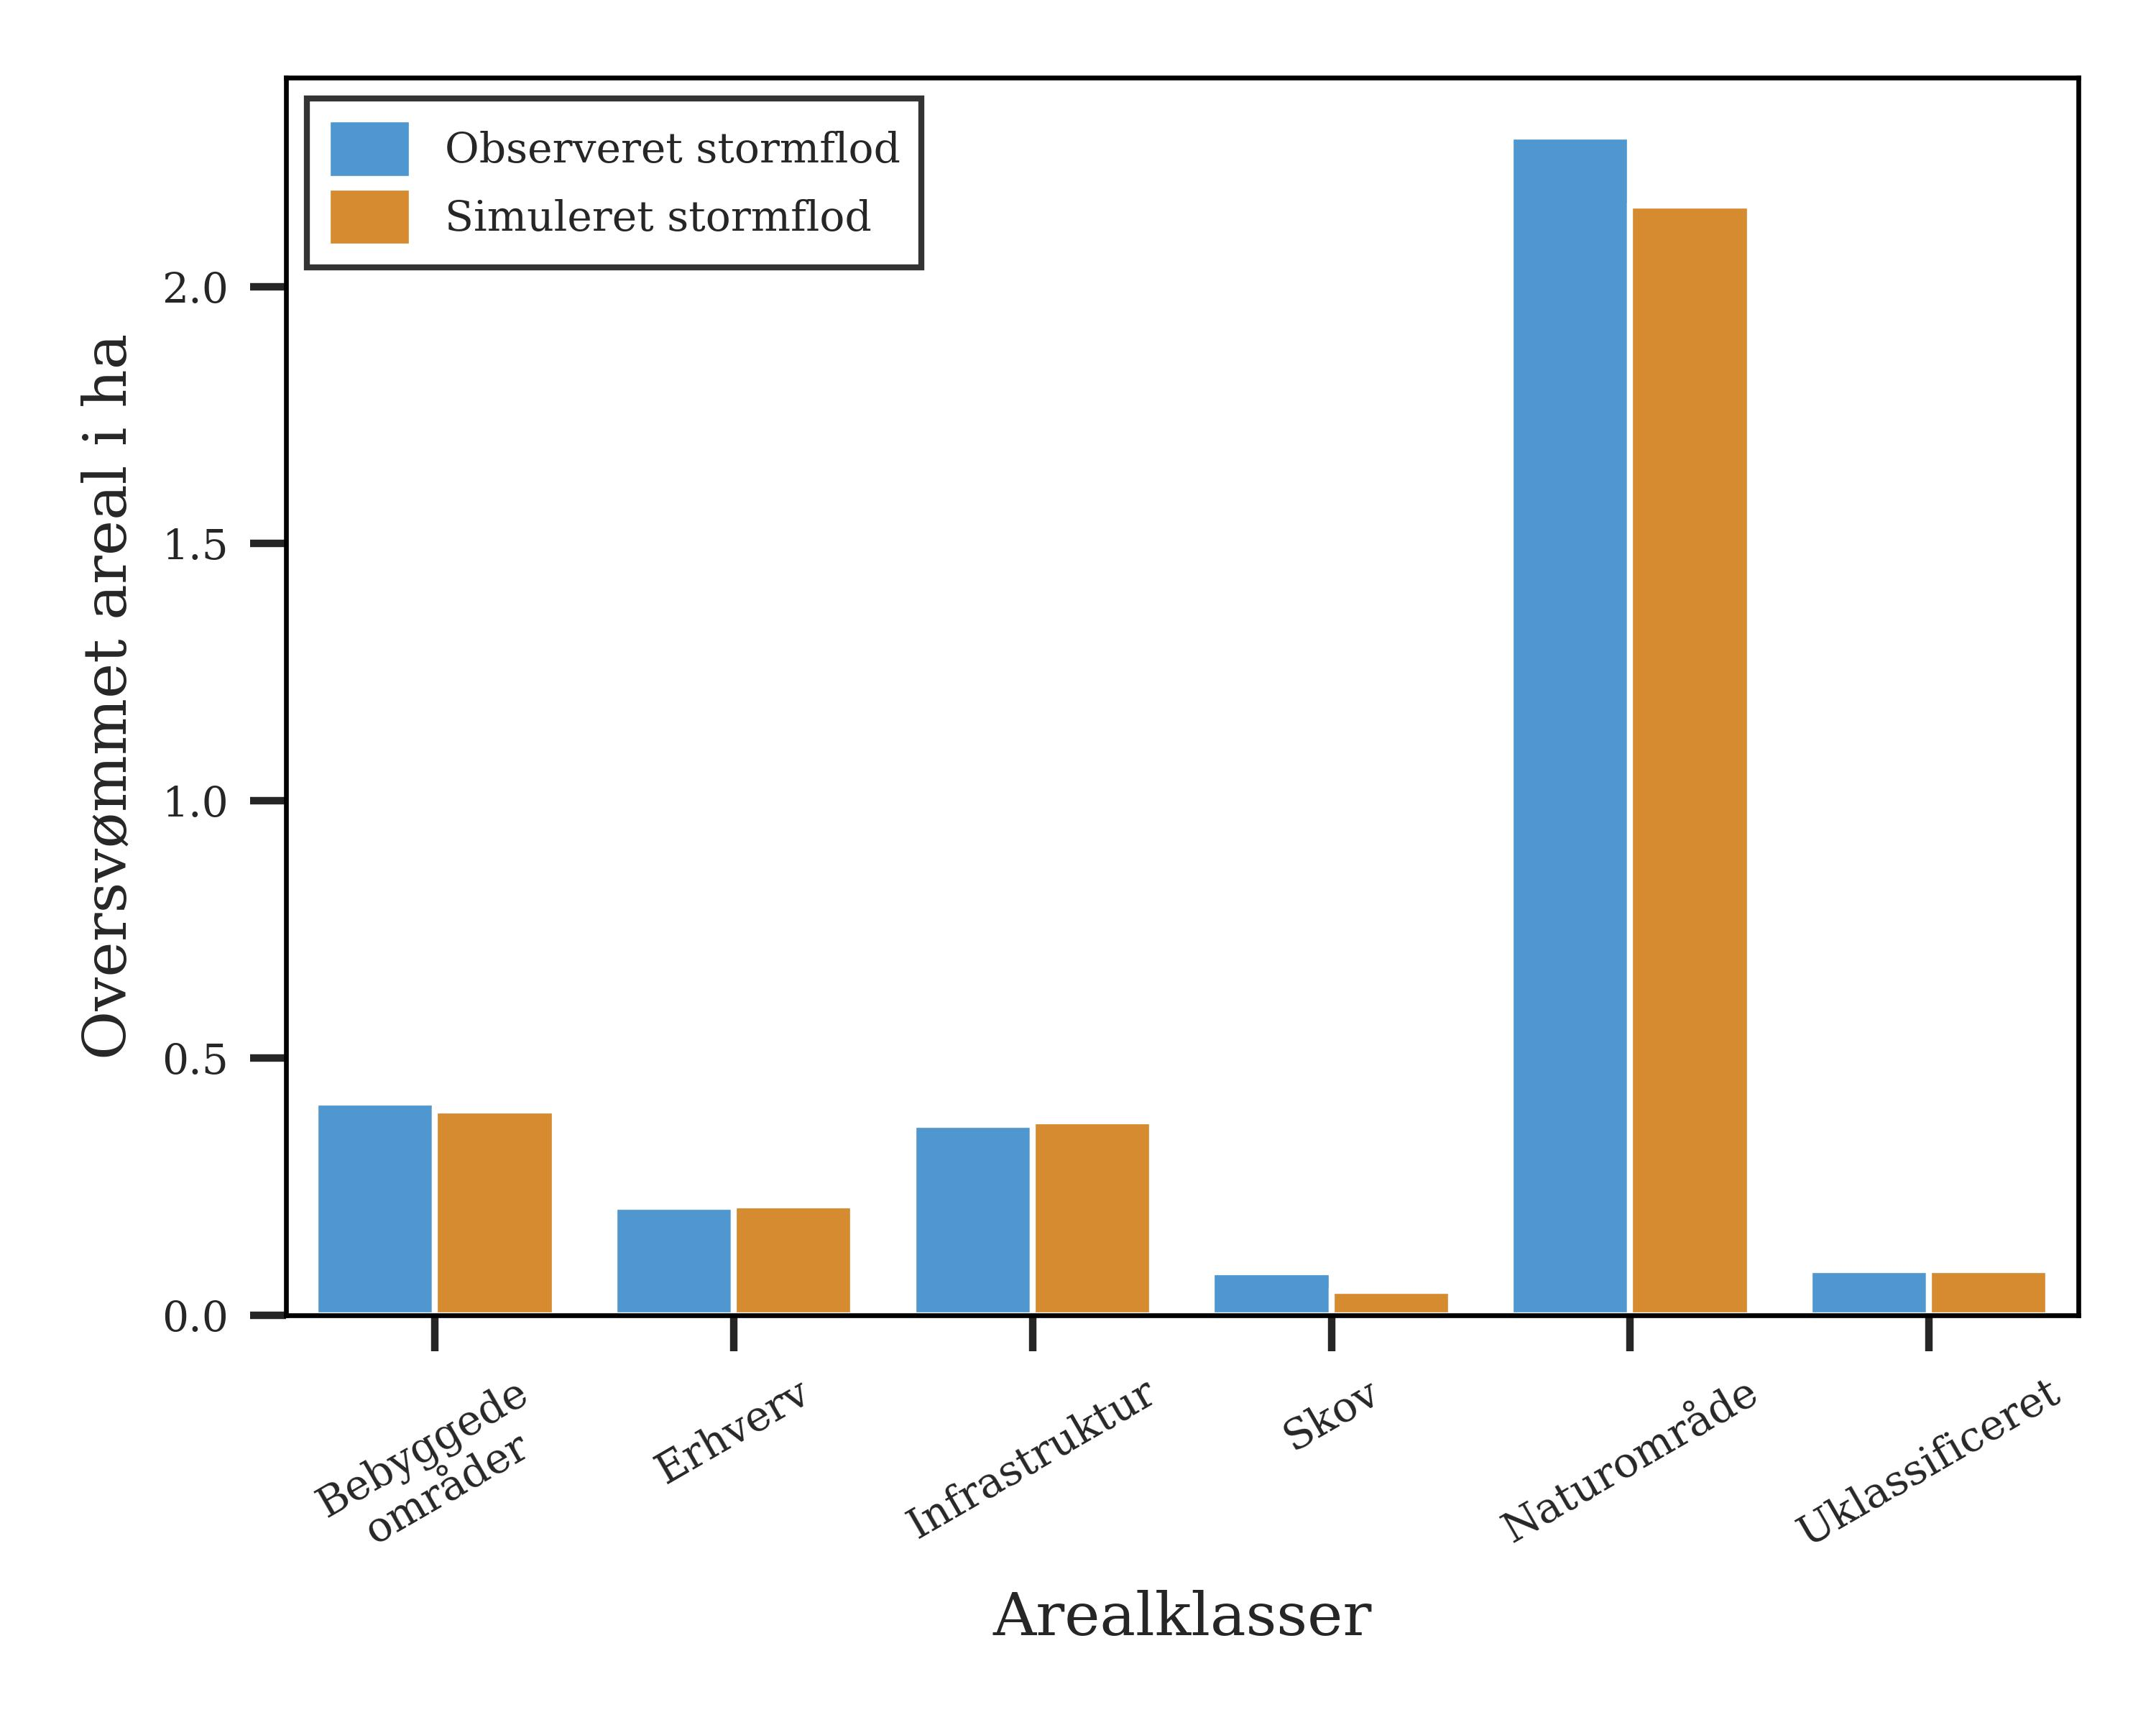
\includegraphics[width=1\linewidth]{images/Resultater/areal_anvendelses_grafer/hesnaes_oversvommet_Hektar.jpg}
        \caption{}
        \label{Subfig: Hektar Hesnæs}
    \end{subfigure}
    \caption{Påvirkede arealanvendelsesklasser i Hesnæs for den observeret og simuleret stormflod. \textbf{(a)} Oversømmet areal som procent af det totale areal. \textbf{(b)} Oversvømmet areal i hektar.}
    \label{Figur: Påvirket arealanvendelse Hesnæs}
\end{figure}


Figur \ref{Figur: Målt & simuleret Præstø} viser den observeret stormflods hændelse og den simuleret hændelse i Præstø. Begge kort viser at kysten og havnen af Præstø bliver oversvømmet samt den nordlige bydel. Den primære forskel mellem de to oversvømmelseskort er at under den observeret hændelse blev en del af Tubæk Ådal oversvømmet samt de omkringliggende arealer. Den observeret hændelse på 53,5 ha er derfor 26\% større i udbredelse end det simuleret resultat på 39.8 ha. Dette svarer til forskel på 13,7 ha. 

\begin{figure}[H]
    \begin{subfigure}[t]{0.5\textwidth}
        \centering
        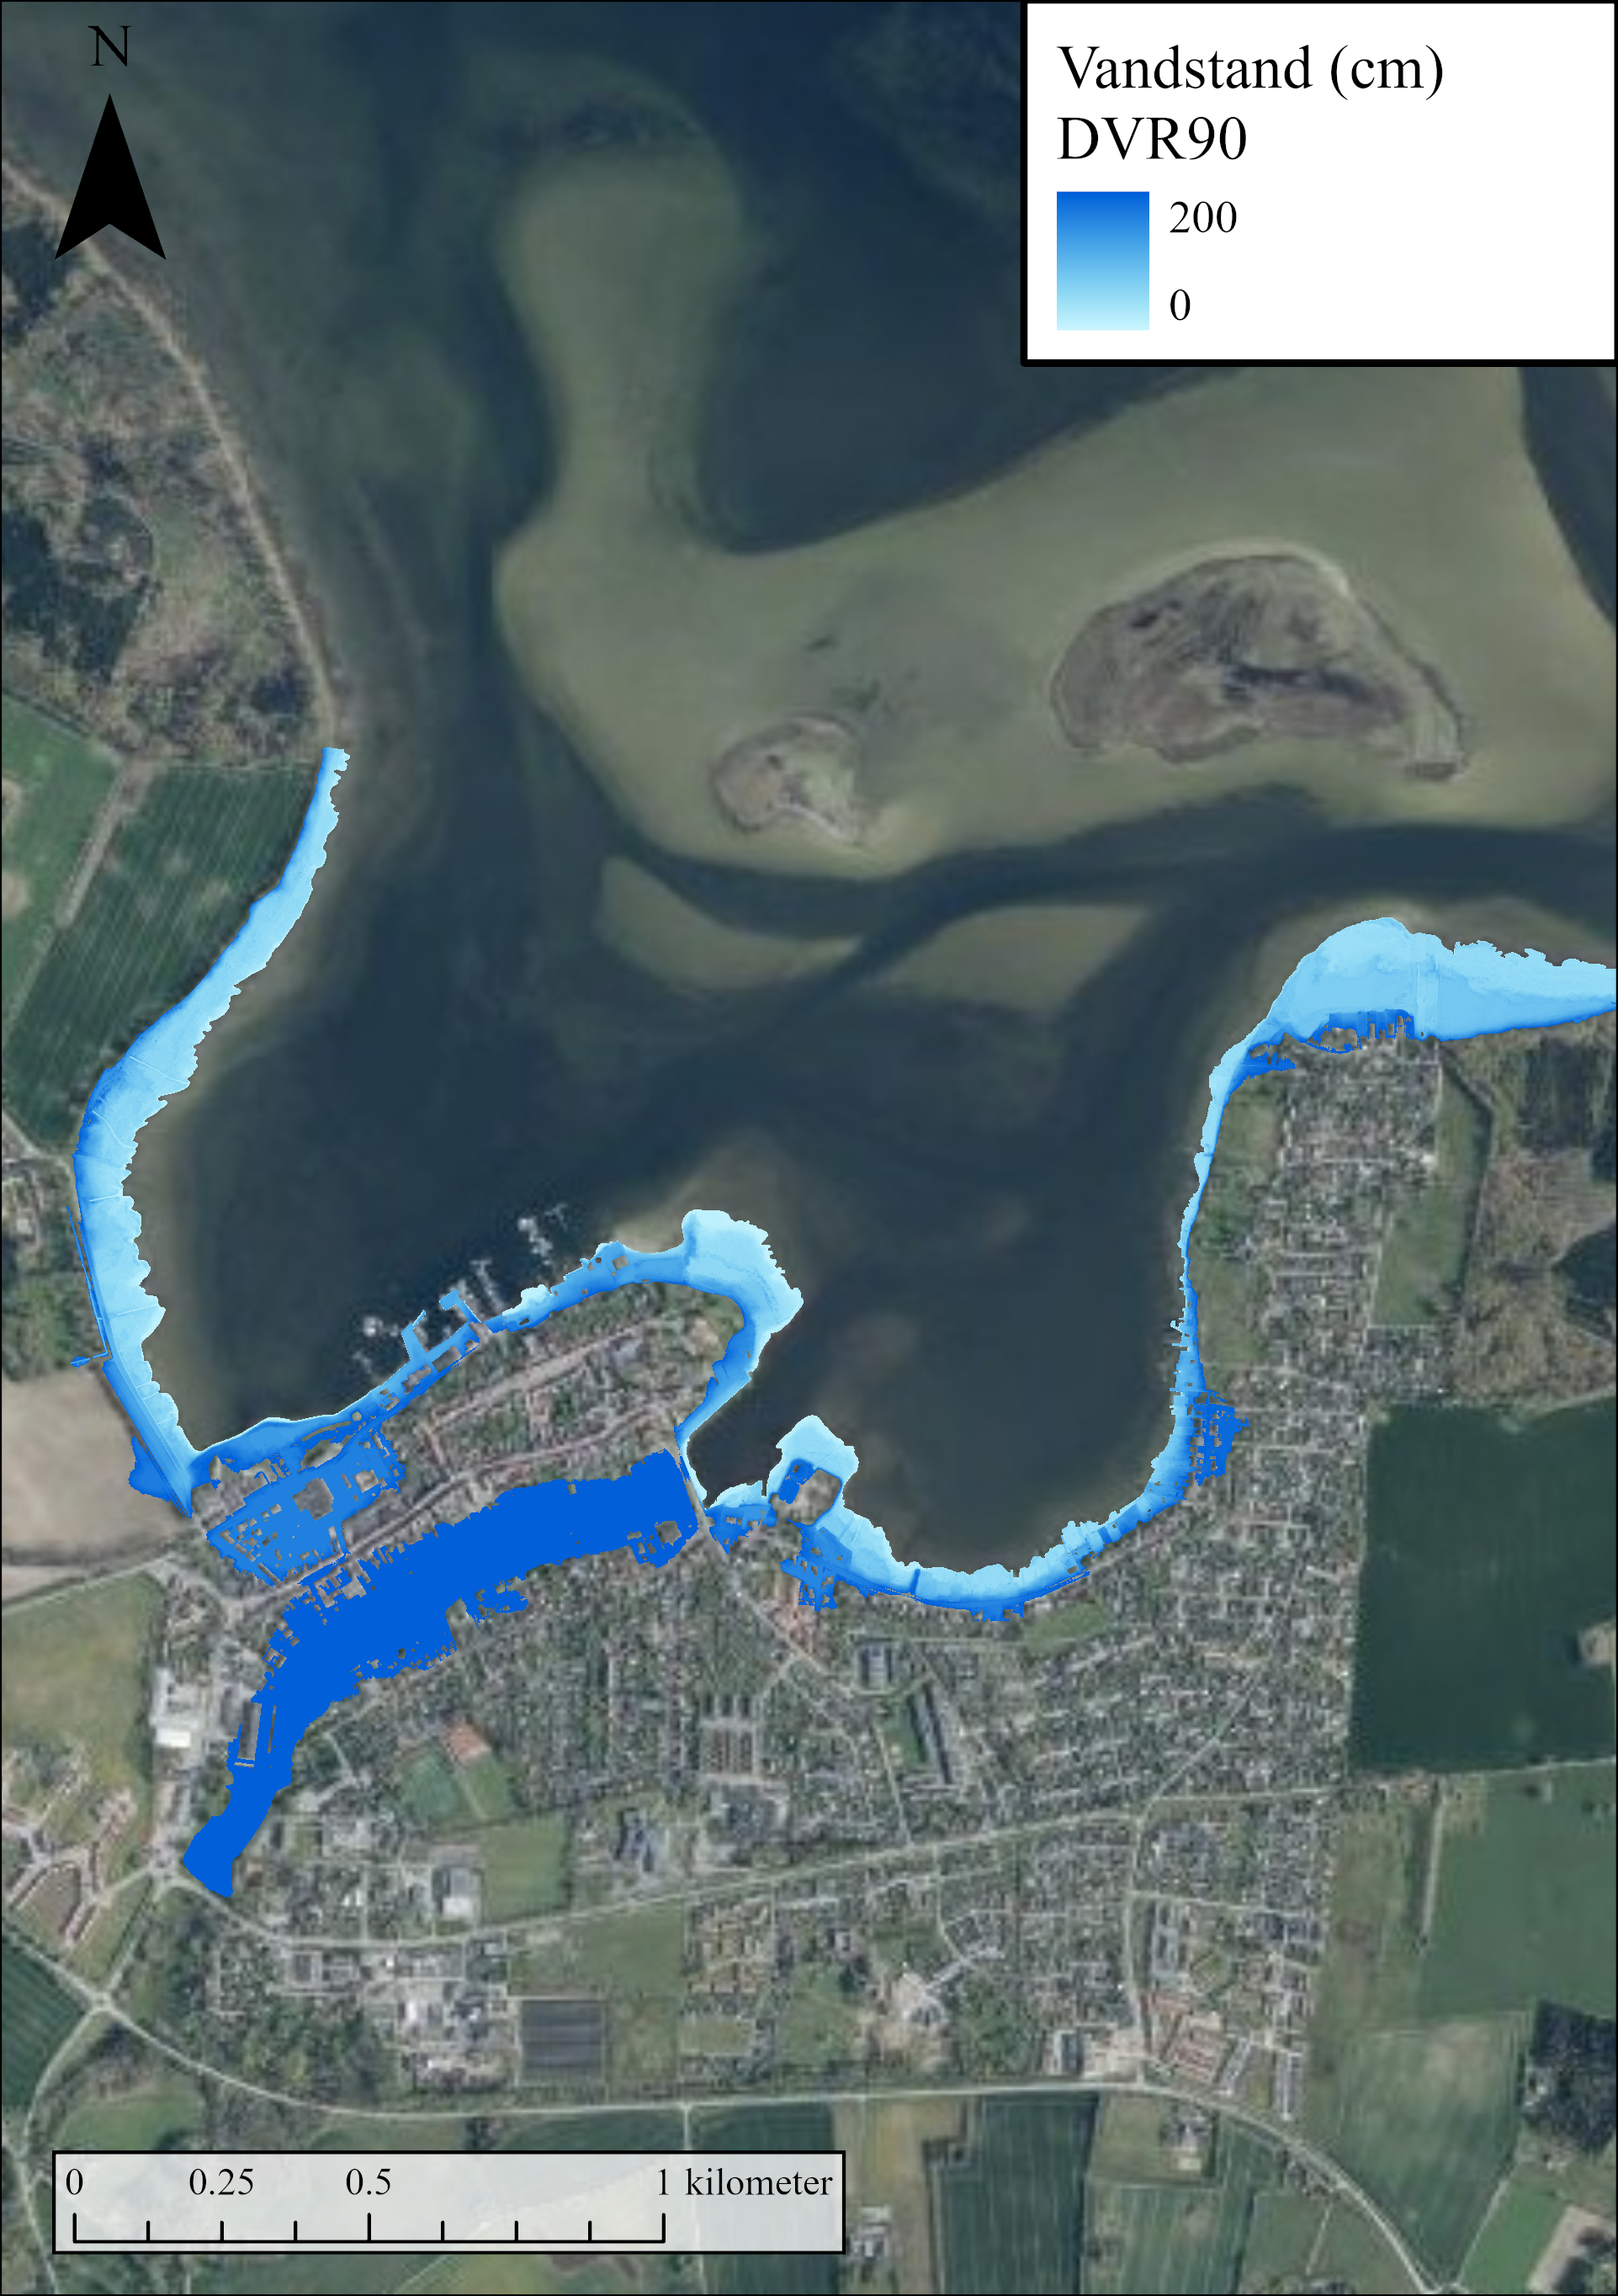
\includegraphics[width=0.95\linewidth]{images/Resultater/2023Malt/2023 resultat_praestoe.jpg}
        \caption{}
        \label{Subfig: Målt Præstø}
    \end{subfigure}
    \begin{subfigure}[t]{0.5\textwidth}
        \centering
        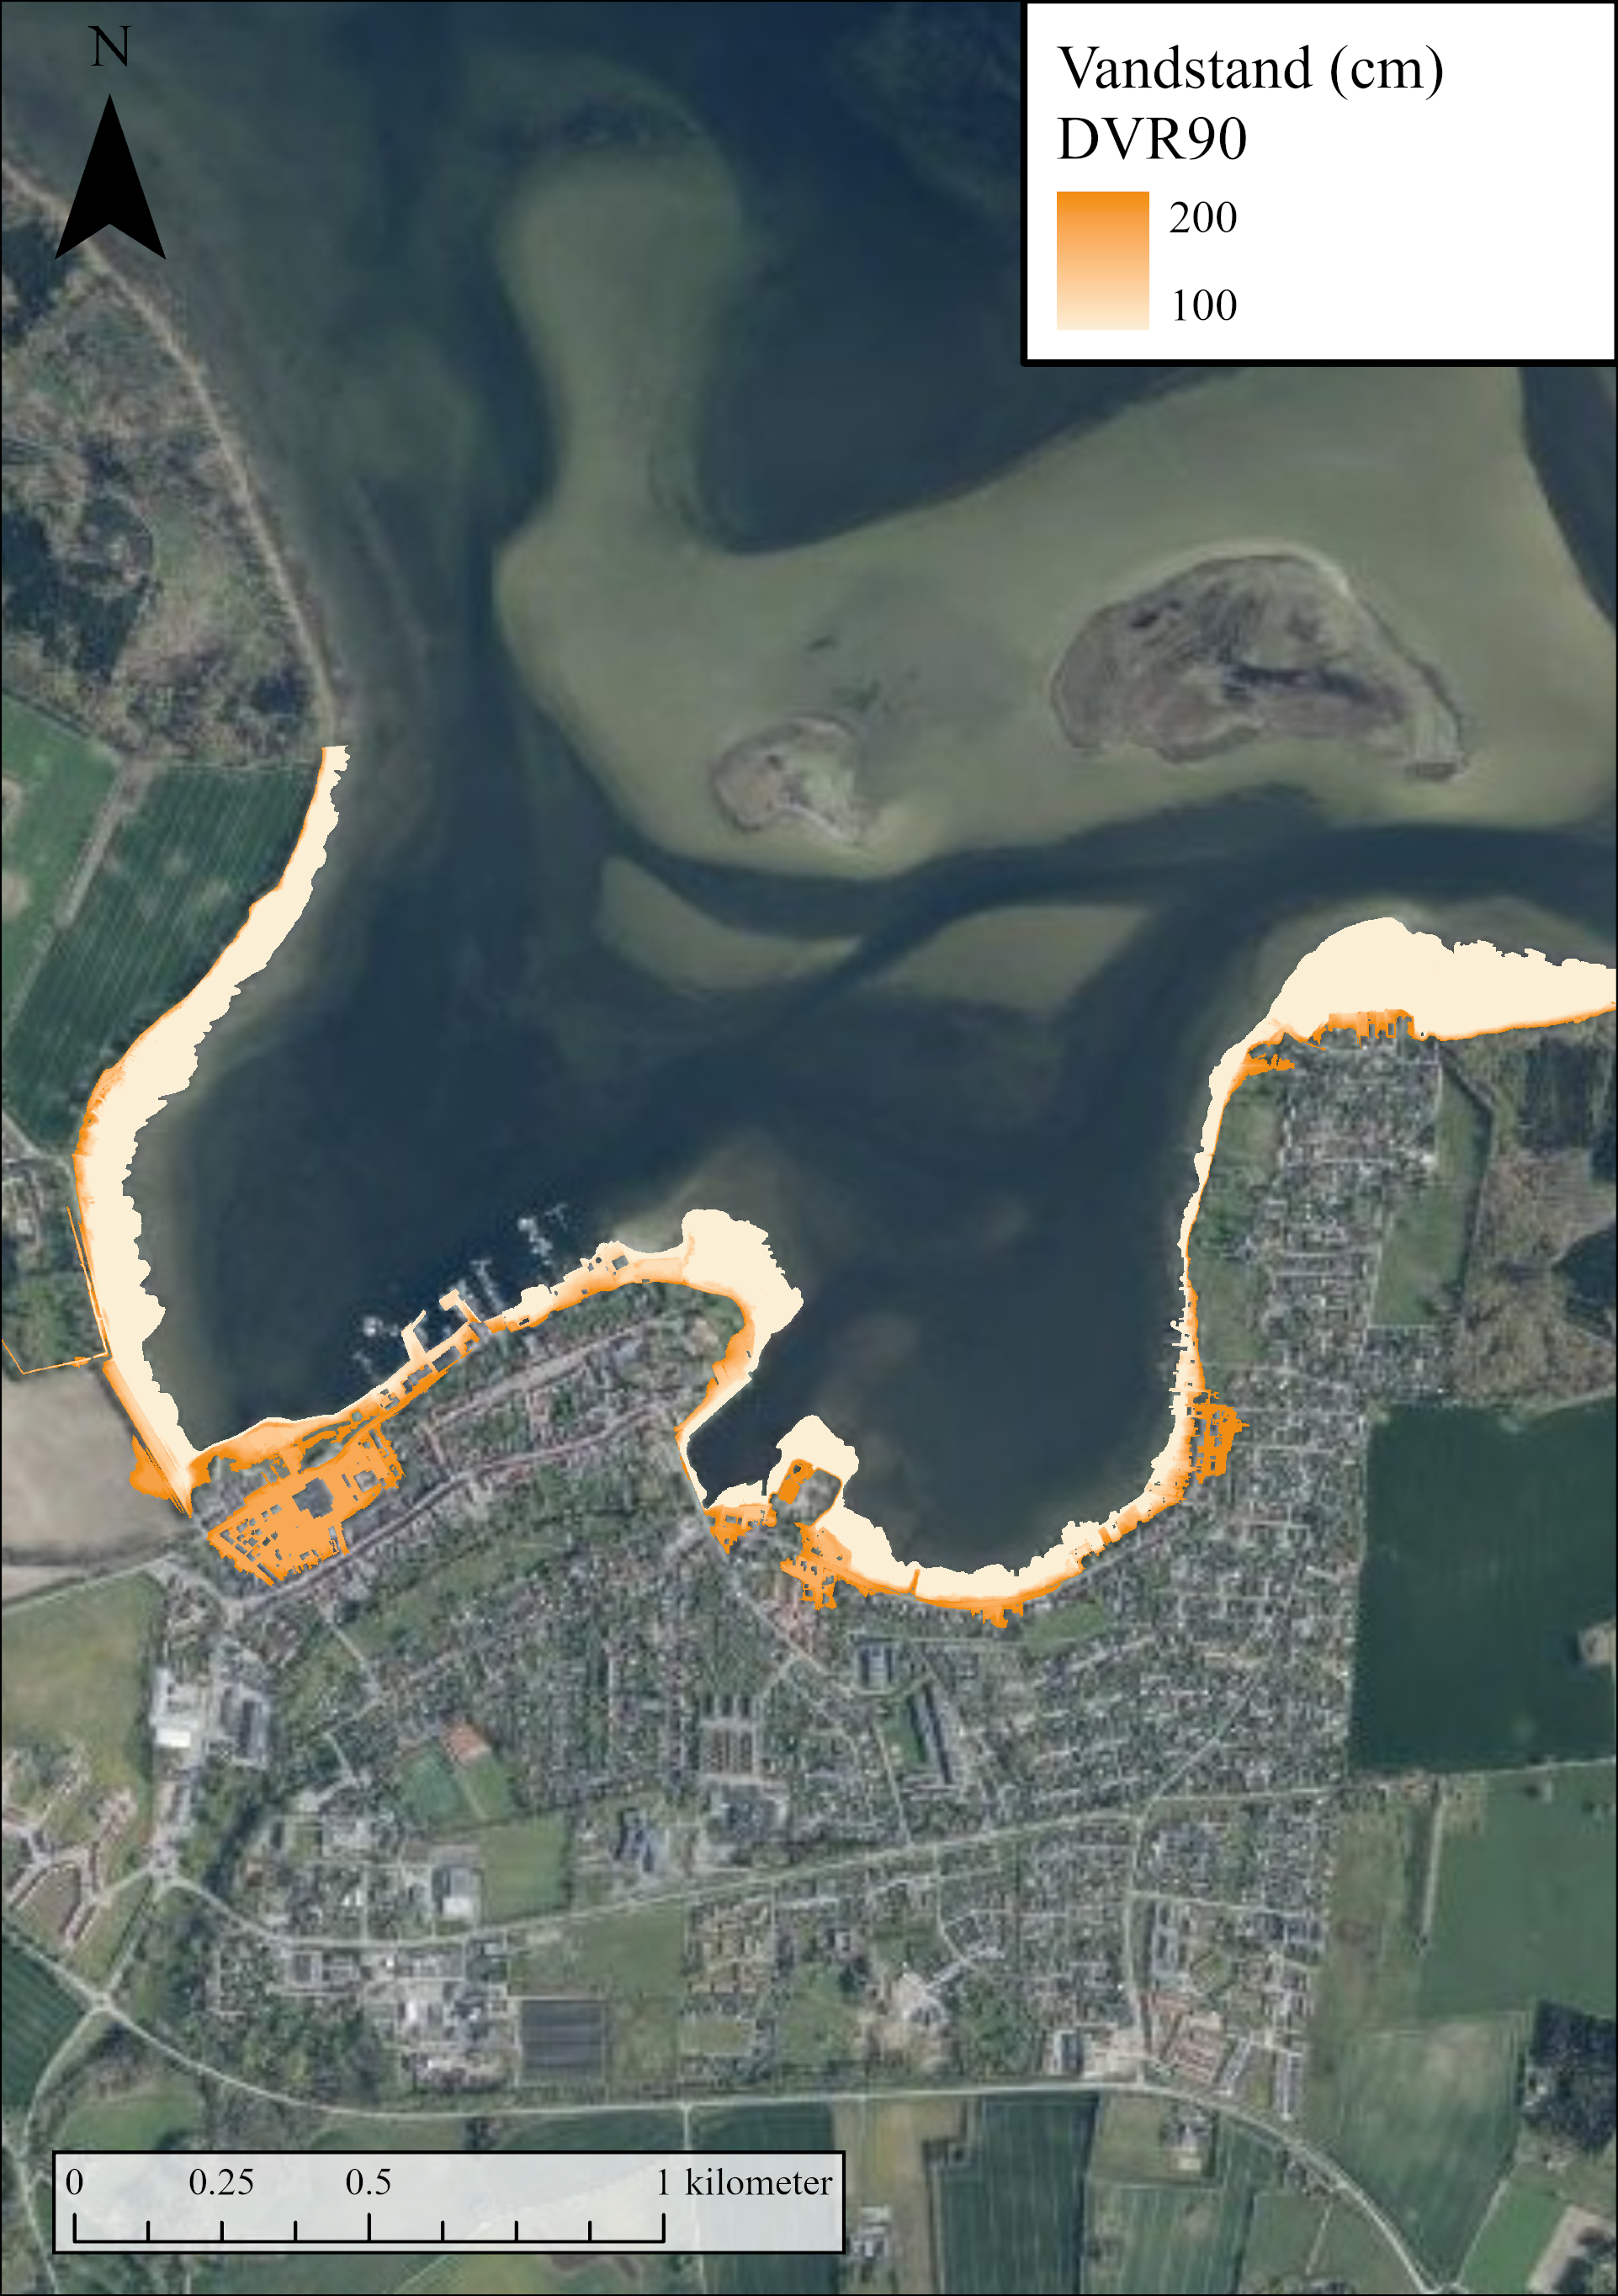
\includegraphics[width=0.95\linewidth]{images/Resultater/2023Model/2023 model_praestoe.jpg}
        \caption{}
        \label{Subfig: Model Præstø}
    \end{subfigure}
    \caption{Oversvømmelseskort over oktober 2023 stormfloden for Præstø. \textbf{(a)} Observeret data. \textbf{(b)} Simuleret data}
    \label{Figur: Målt & simuleret Præstø}
\end{figure}

I Præstø blev otte forskellige arealanvendelser påvirket af stormfloden. For både den observeret og simuleret hændelse var naturområde det mest påvirket areal med 47 og 60\% henholdsvis. Da den observeret oversvømmelse er et større areal udgør naturområder en mindre andel af det totale areal end for den simuleret hændelse (figur \ref{Subfig: Procent præstø}). Den observeret hændelse havde et større rekreativt område oversvømmet end den simuleret hændelse med en forskel på 4 ha, da arealerne langs Tubæk Ådal er klassificeret som rekreative områder. Grundet oversvømmelsen af Tubæk Ådal er et større bebygget areal blevet oversvømmet med ca. 12 ha i den observeret stormflod og 6 ha i den simuleret stormflod. Det samme er gældende for infrastruktur og erhvervs områder (figur \ref{Subfig: Hektar præstø}).
\begin{figure}[H]
    \begin{subfigure}[b]{0.5\textwidth}
        \centering
        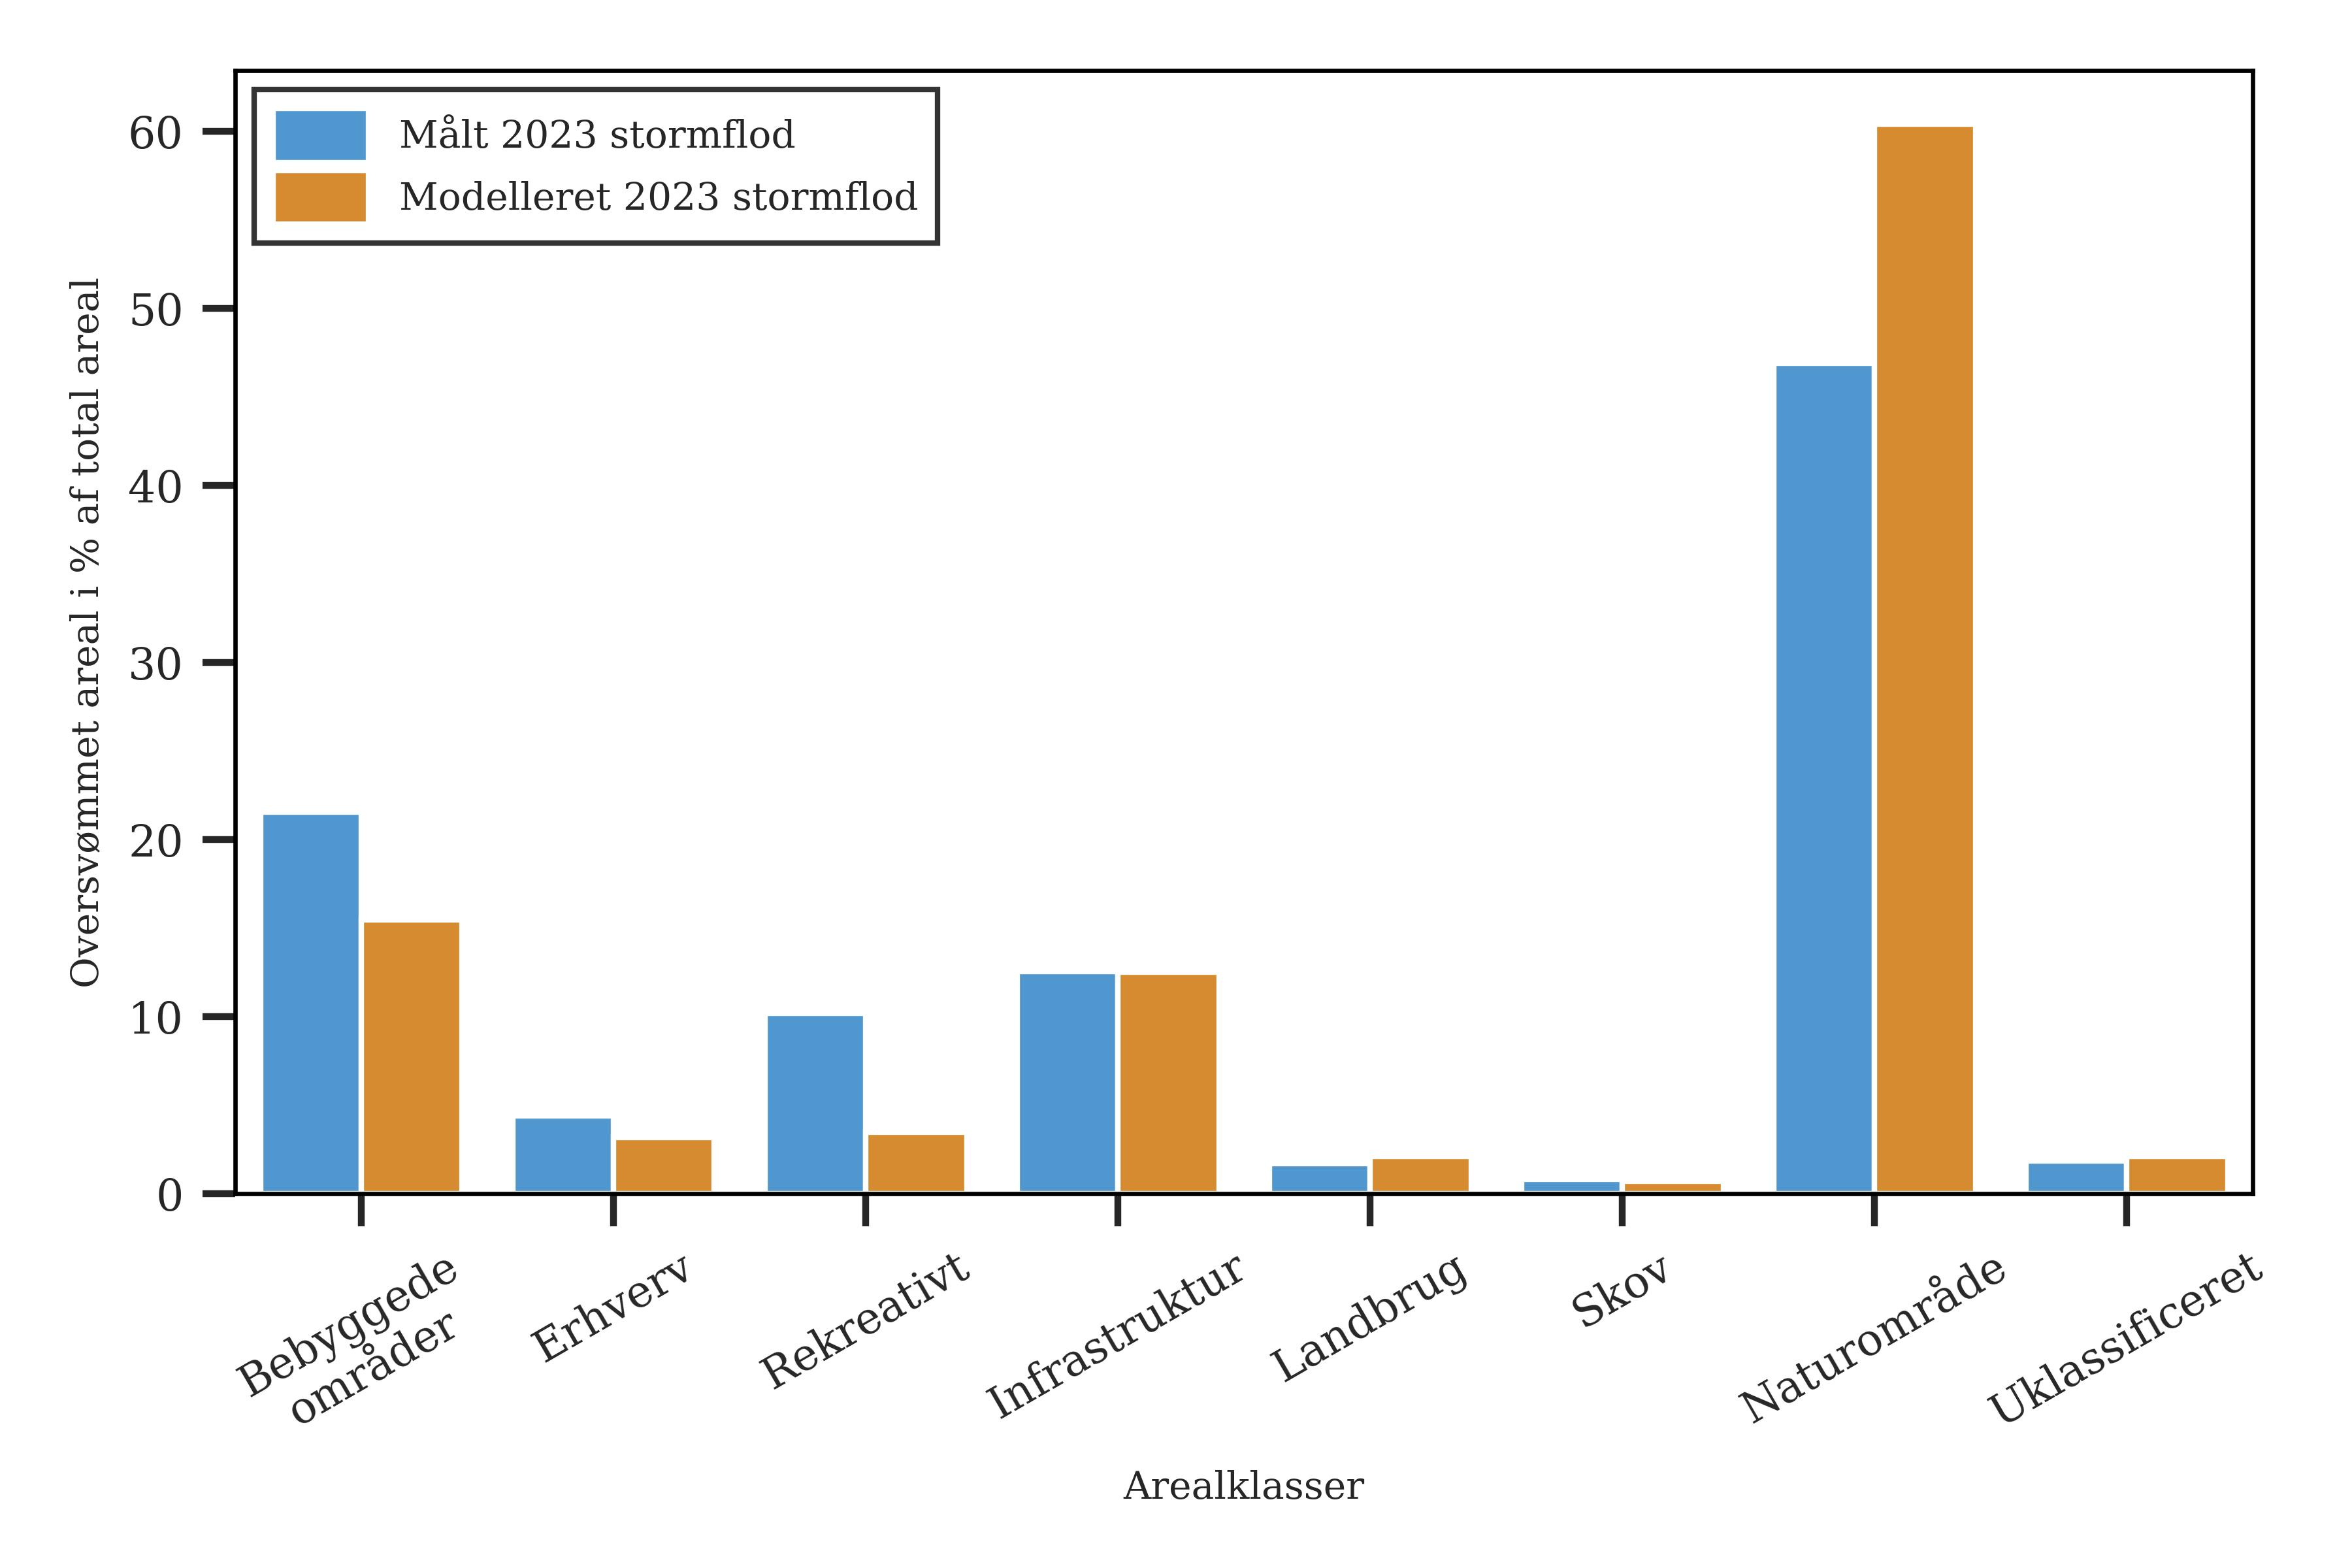
\includegraphics[width=1\linewidth]{images/Resultater/areal_anvendelses_grafer/praestoe_arealanvendelse.jpg}
        \caption{}
        \label{Subfig: Procent præstø}
    \end{subfigure}
    \begin{subfigure}[b]{0.5\textwidth}
        \centering
        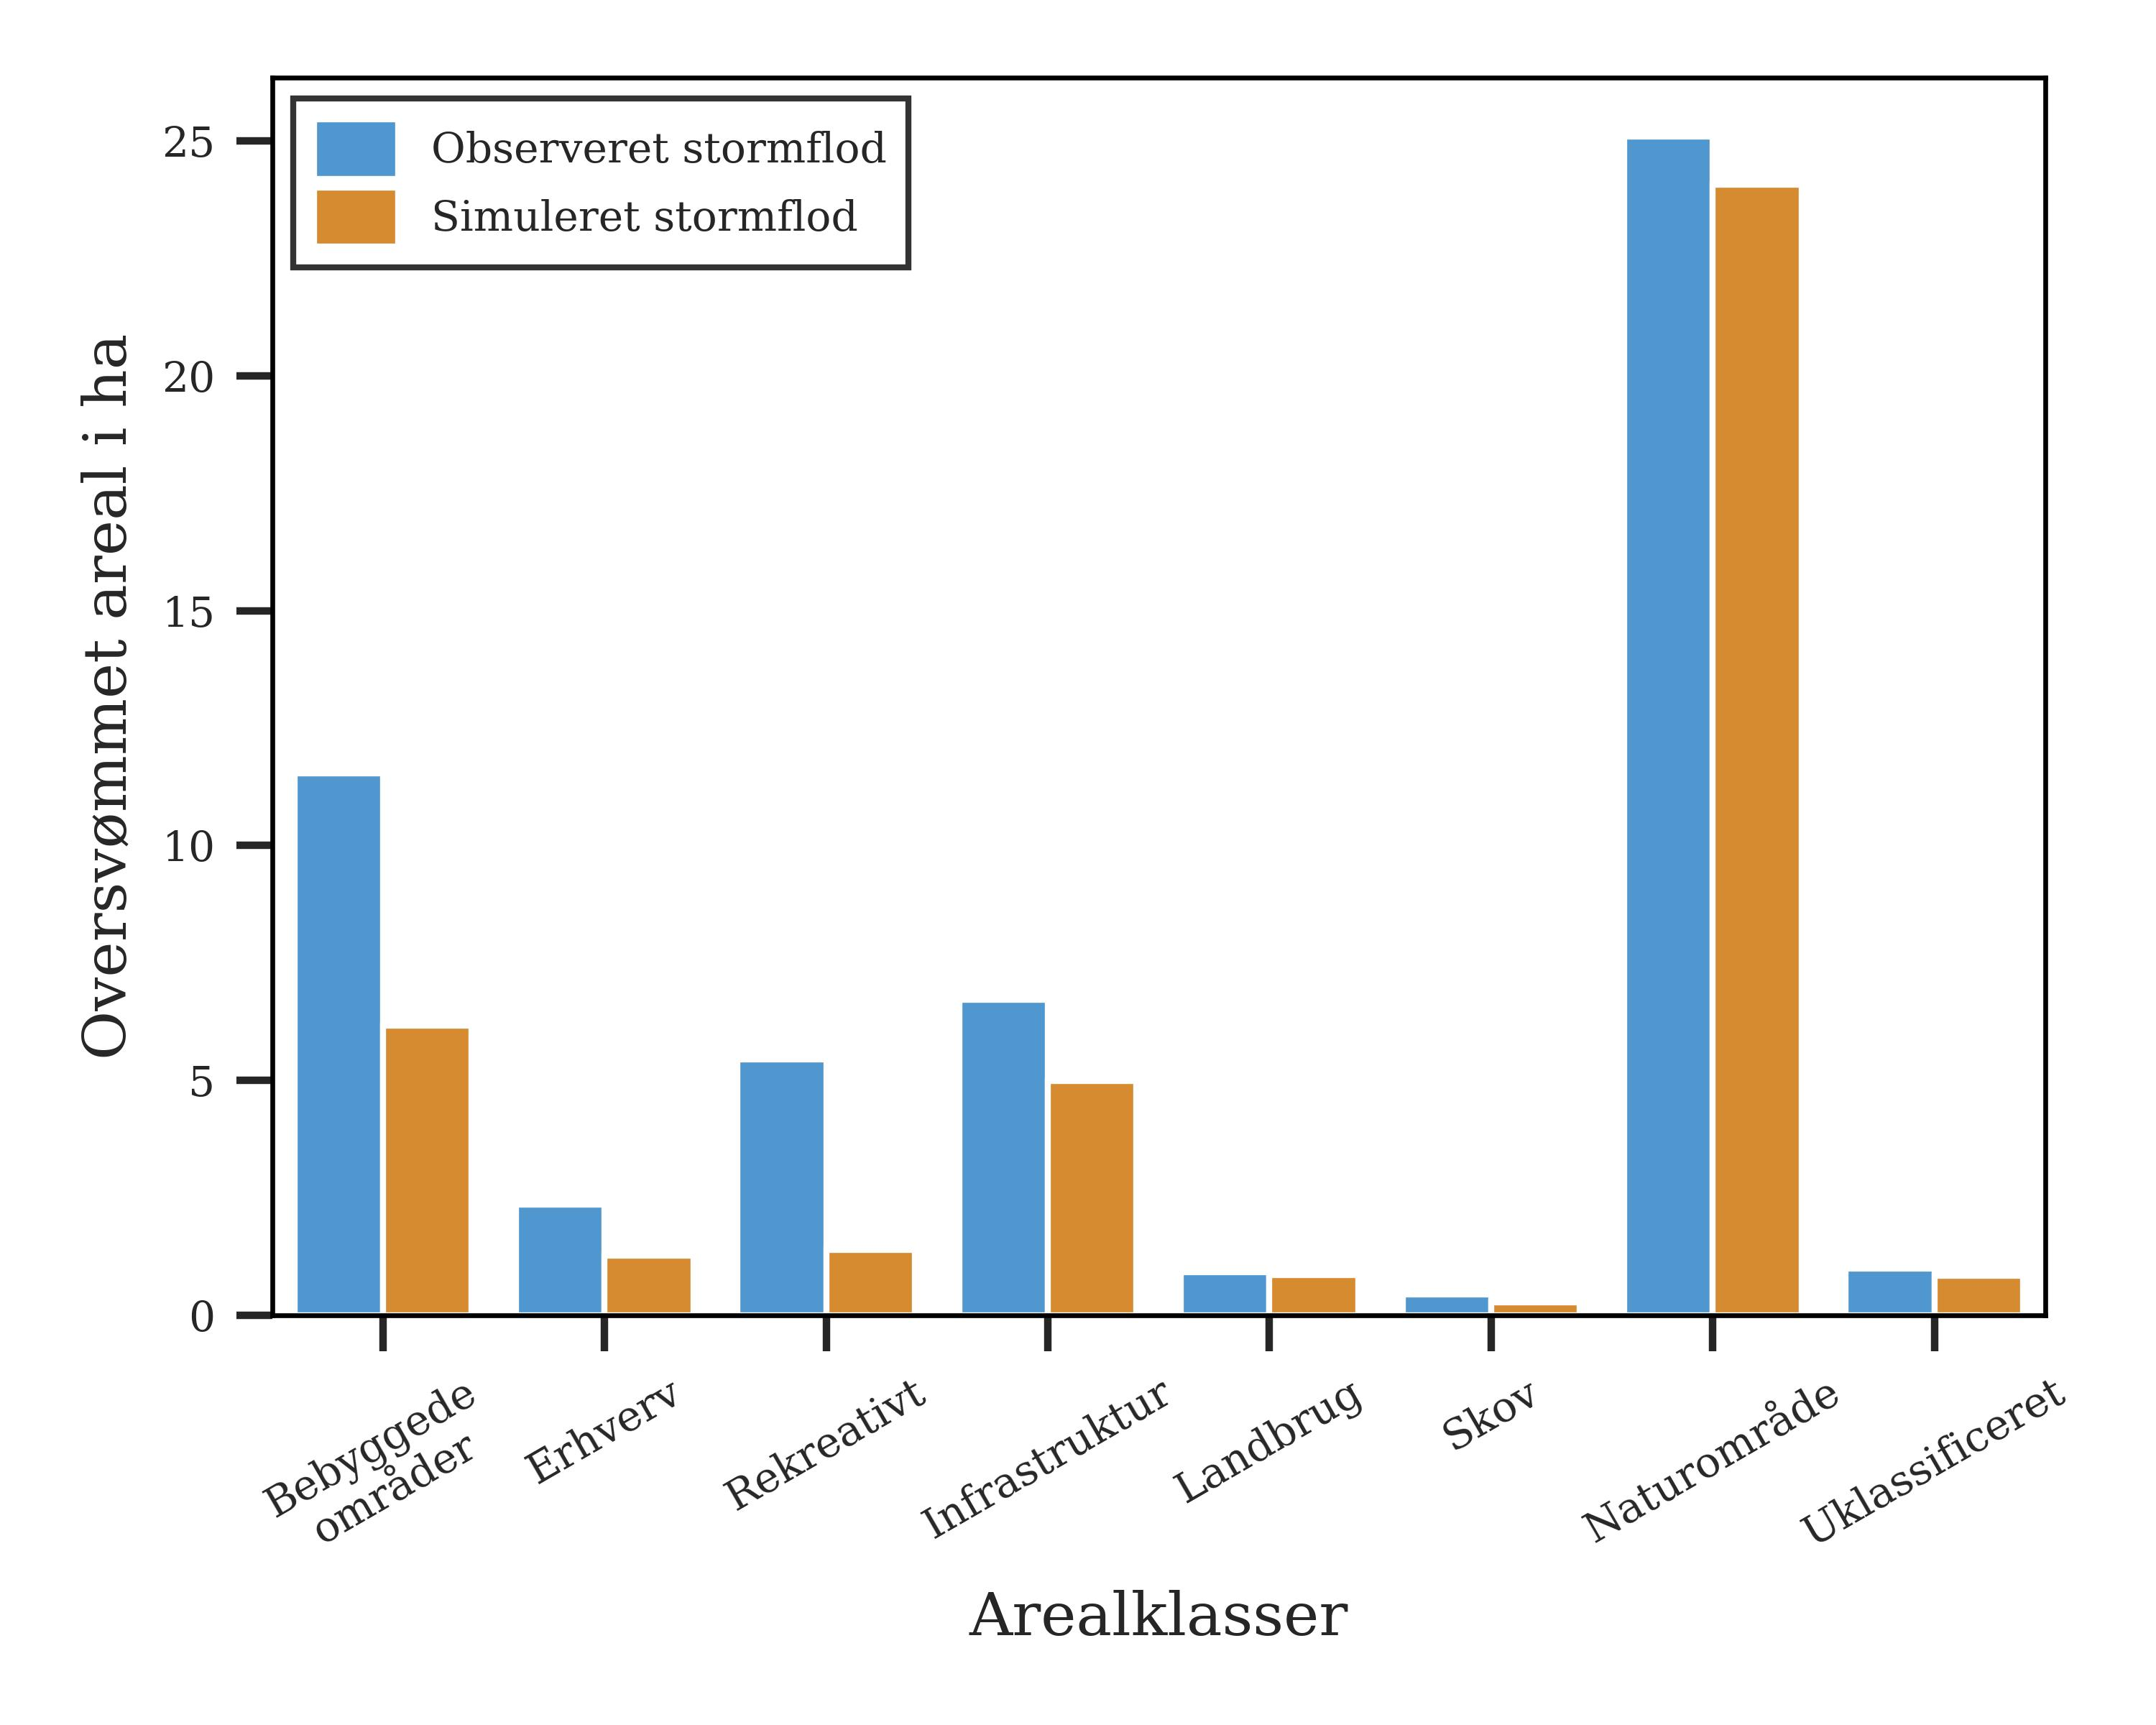
\includegraphics[width=1\linewidth]{images/Resultater/areal_anvendelses_grafer/praestoe_oversvommet_Hektar.jpg}
        \caption{}
        \label{Subfig: Hektar præstø}
    \end{subfigure}
    \caption{Påvirkede arealanvendelsesklasser i Præstø for den observeret og simuleret stormflod. \textbf{(a)} Oversømmet areal som procent af det totale areal. \textbf{(b)} Oversvømmet areal i hektar.}
    \label{Figur: Påvirket arealanvendelse Præstø}
\end{figure}


\newpage
\subsection{Fremskrevet og statistiske stormflods hændelser}

I dette afsnit vil der blive præsenteret resultaterne af en 100-års hændelse og en fremskrivning af 2023-stormfloden i slutningen af det nuværende århundrede ved et SSP4,5 og 8,5 udledningsscenarie. 
\begin{figure}[H]
    \centering
    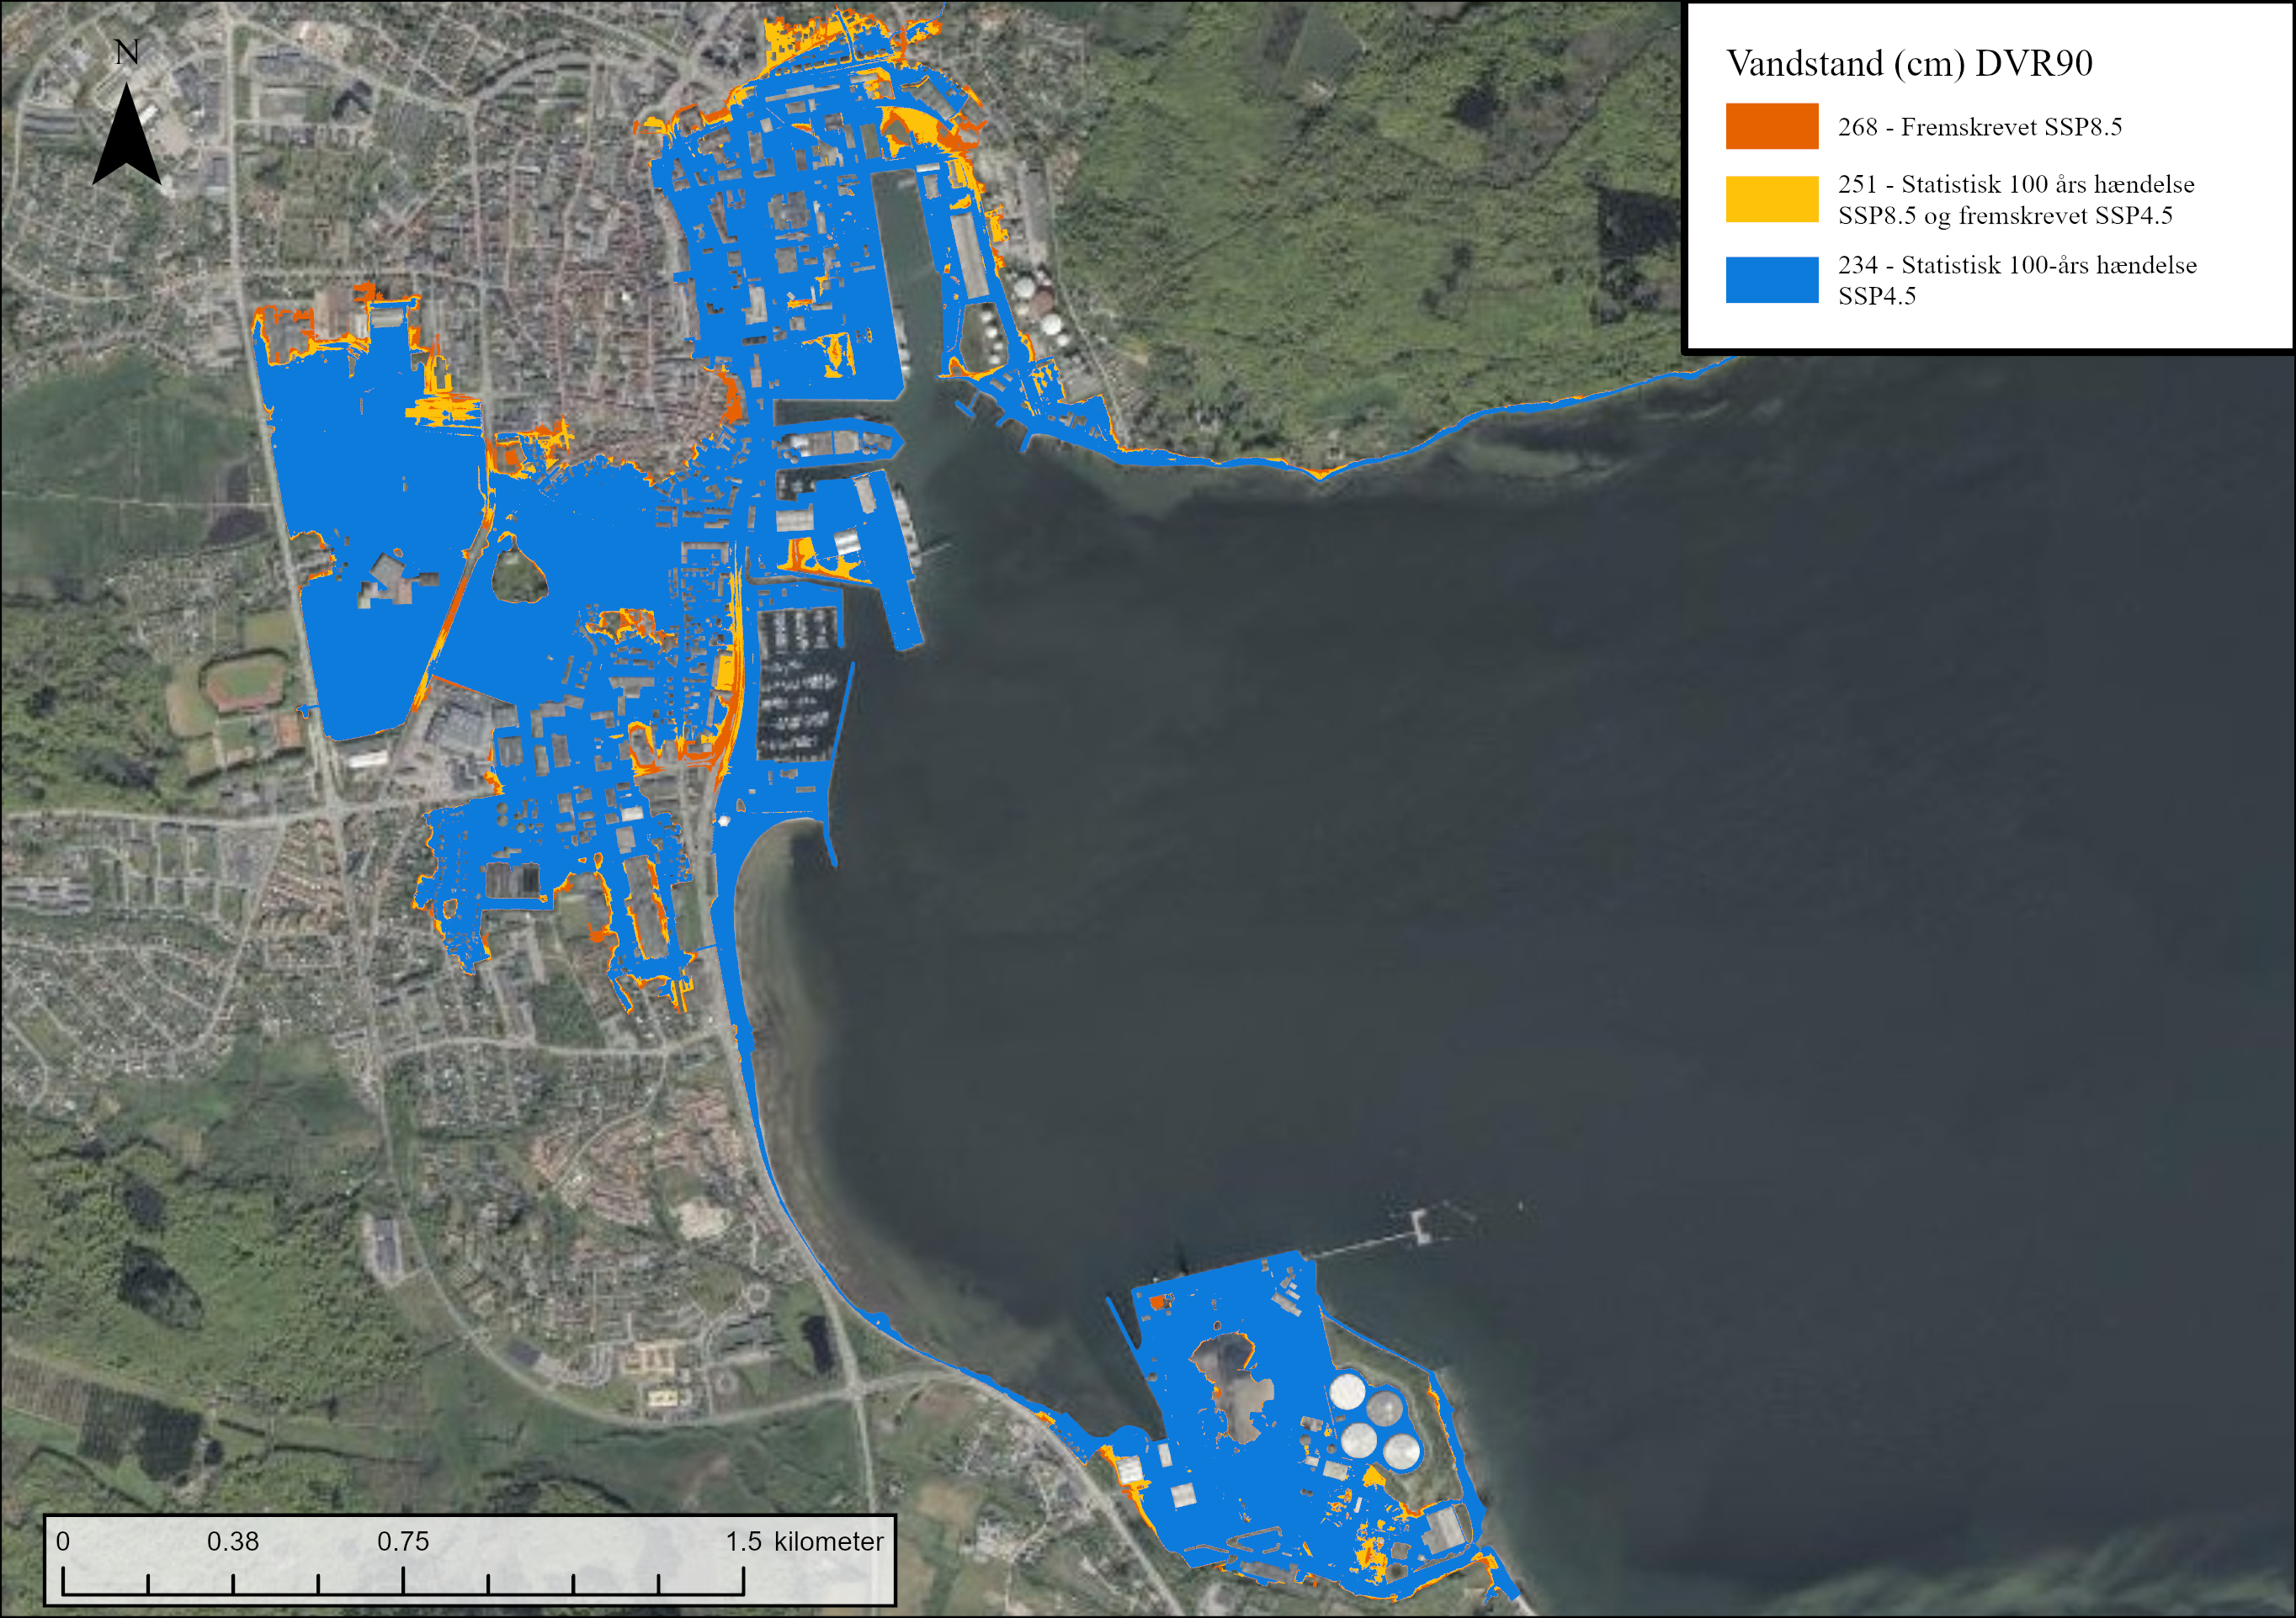
\includegraphics[width=0.8\linewidth]{images/Resultater/fremskrevet_hændelser/klima resultat_aabenraa.jpg}
    \caption{Kort over oversvømmet areal i Aabenraa af en stormflod ved en statistisk 100-års hændelse og en fremskrivning af 2023-stormfloden til slutningen af århundredet ved et SSP4,5 og SSP8,5 scenarie.}
    \label{Figur: Klima Aabenraa}
\end{figure}
I figur \ref{Figur: Klima Aabenraa} ses et oversvømmelseskort over Aabenraa for en 100-års hændelse og en fremskrivning af stormfloden ved et SSP4,5 og SSP8,5 scenarie. Det største areal oversvømmet sker ved en 100-års hændelse i SSP4,5 med en vandstand på 234 cm over DVR90 hvor en større del af den sydlige bydel bliver oversvømmet. Det oversvømmet areal ved fremskrivningen af stormfloden i et SSP8,5 scenarie er 13\% større end en 100-års hændelse i SSP4,5. Dette svarer til 19,6 ha. I forhold til den observeret 2023-stormflodshændelse, oversvømmer en fremskrevet stormflod et 96 og 104 ha større areal ved henholdsvis et SSP4,5 og SSP8,5 klimascenarie. Det er primært i den nordelige del af Aabenraa hvor der er forskel mellem 100-års hændelsen og den fremskrevet stormflod.  
\begin{figure}[H]
    \centering
    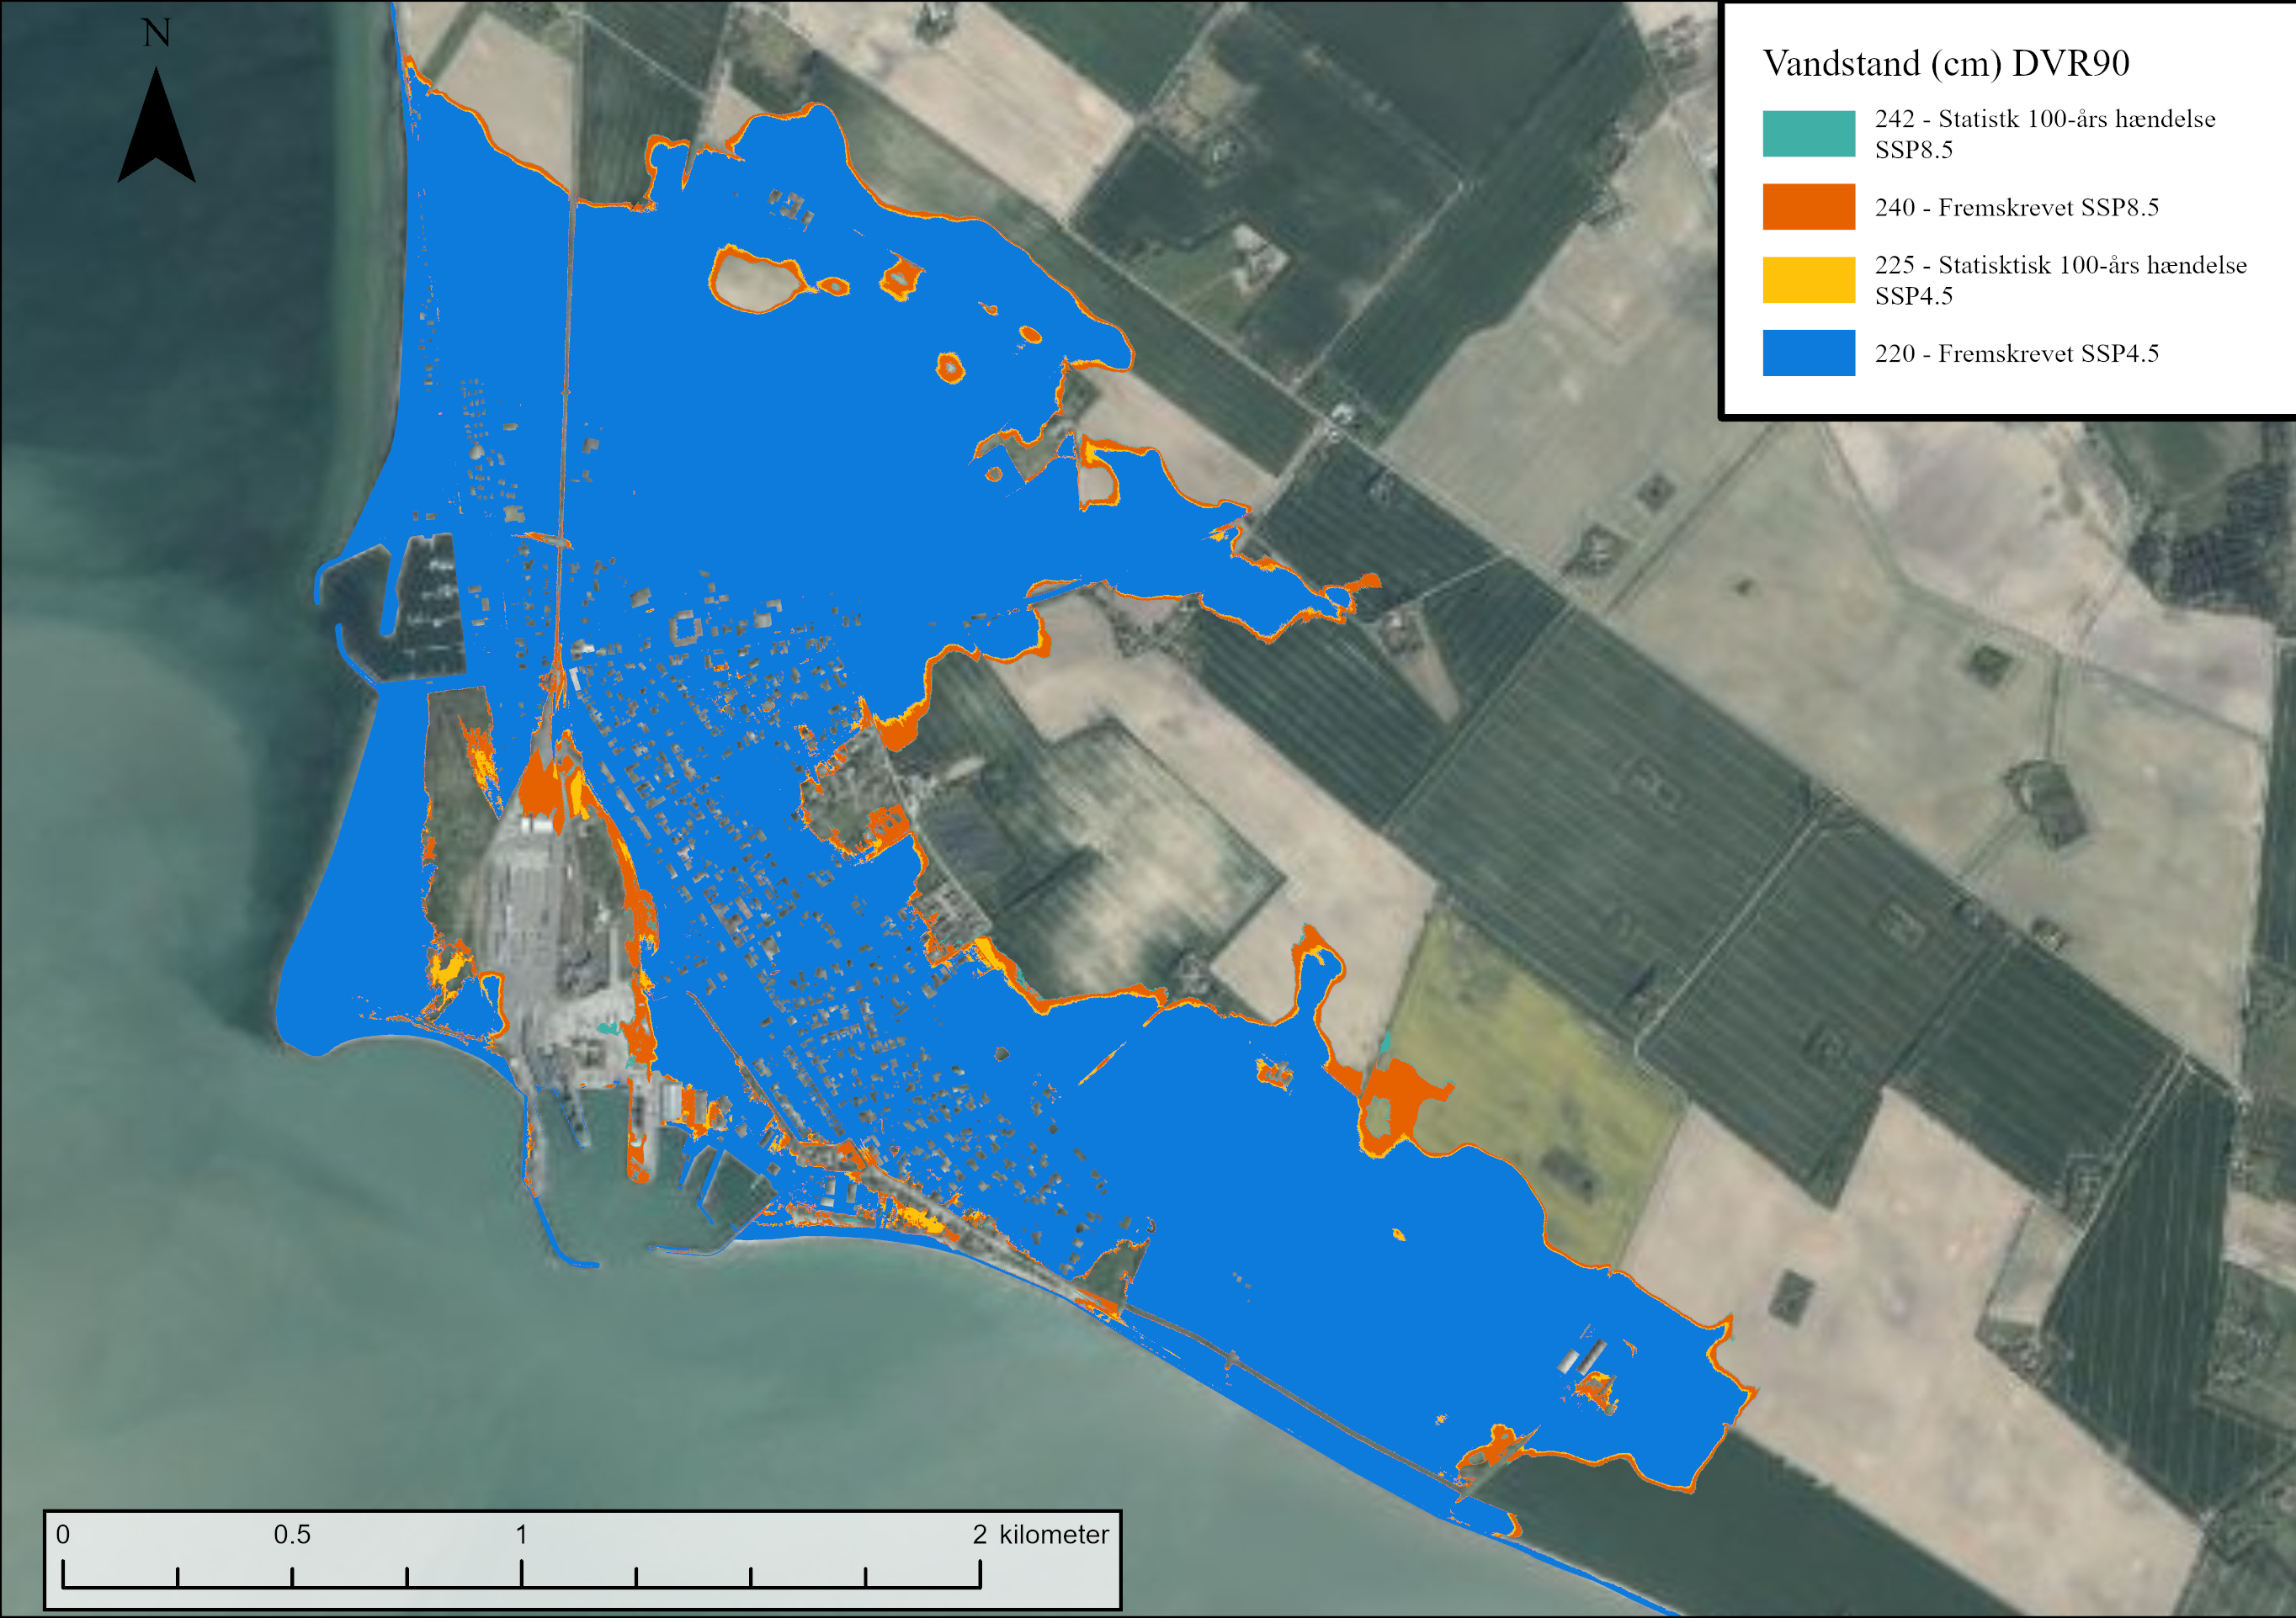
\includegraphics[width=0.8\linewidth]{images/Resultater/fremskrevet_hændelser/klima resultat gedser.jpg}
    \caption{Kort over oversvømmet areal i Gedser Havn af en stormflod ved en statistisk 100-års hændelse og en fremskrivning af oktober 2023 stormfloden til slutningen af århundredet ved et SSP4,5 og SSP8,5 scenarie.}
    \label{Figur: Klima Gedser Havn}
\end{figure}
I figur \ref{Figur: Klima Gedser Havn} er der vist et oversvømmelseskort over Gedser Havn for en 100-års hændelse og fremskrivningen af stormfloden ved et SSP4,5 og 8,5 scenarie. Den største del af oversvømmelsen sker ved en fremskrevet stormflod ved SSP4,5 med en vandstand på 220 cm DVR90. Størstedelen af landsbyen Gedser Havn bliver oversvømmet samt en del af det bagvedliggende landbrugsområder. Ved en 100-års hændelse i et SSP8,5 scenarie er det oversvømmet areal steget til 219,7 ha, en stigning på 537\% i forhold til den stormflod der ramte i 2023. Færgehavnen og terminalen bliver ikke oversvømmet ved nogen af de fire scenarier, dog bliver hovedvejen ind til færgehavnen oversvømmet.
\begin{figure}[H]
    \centering
    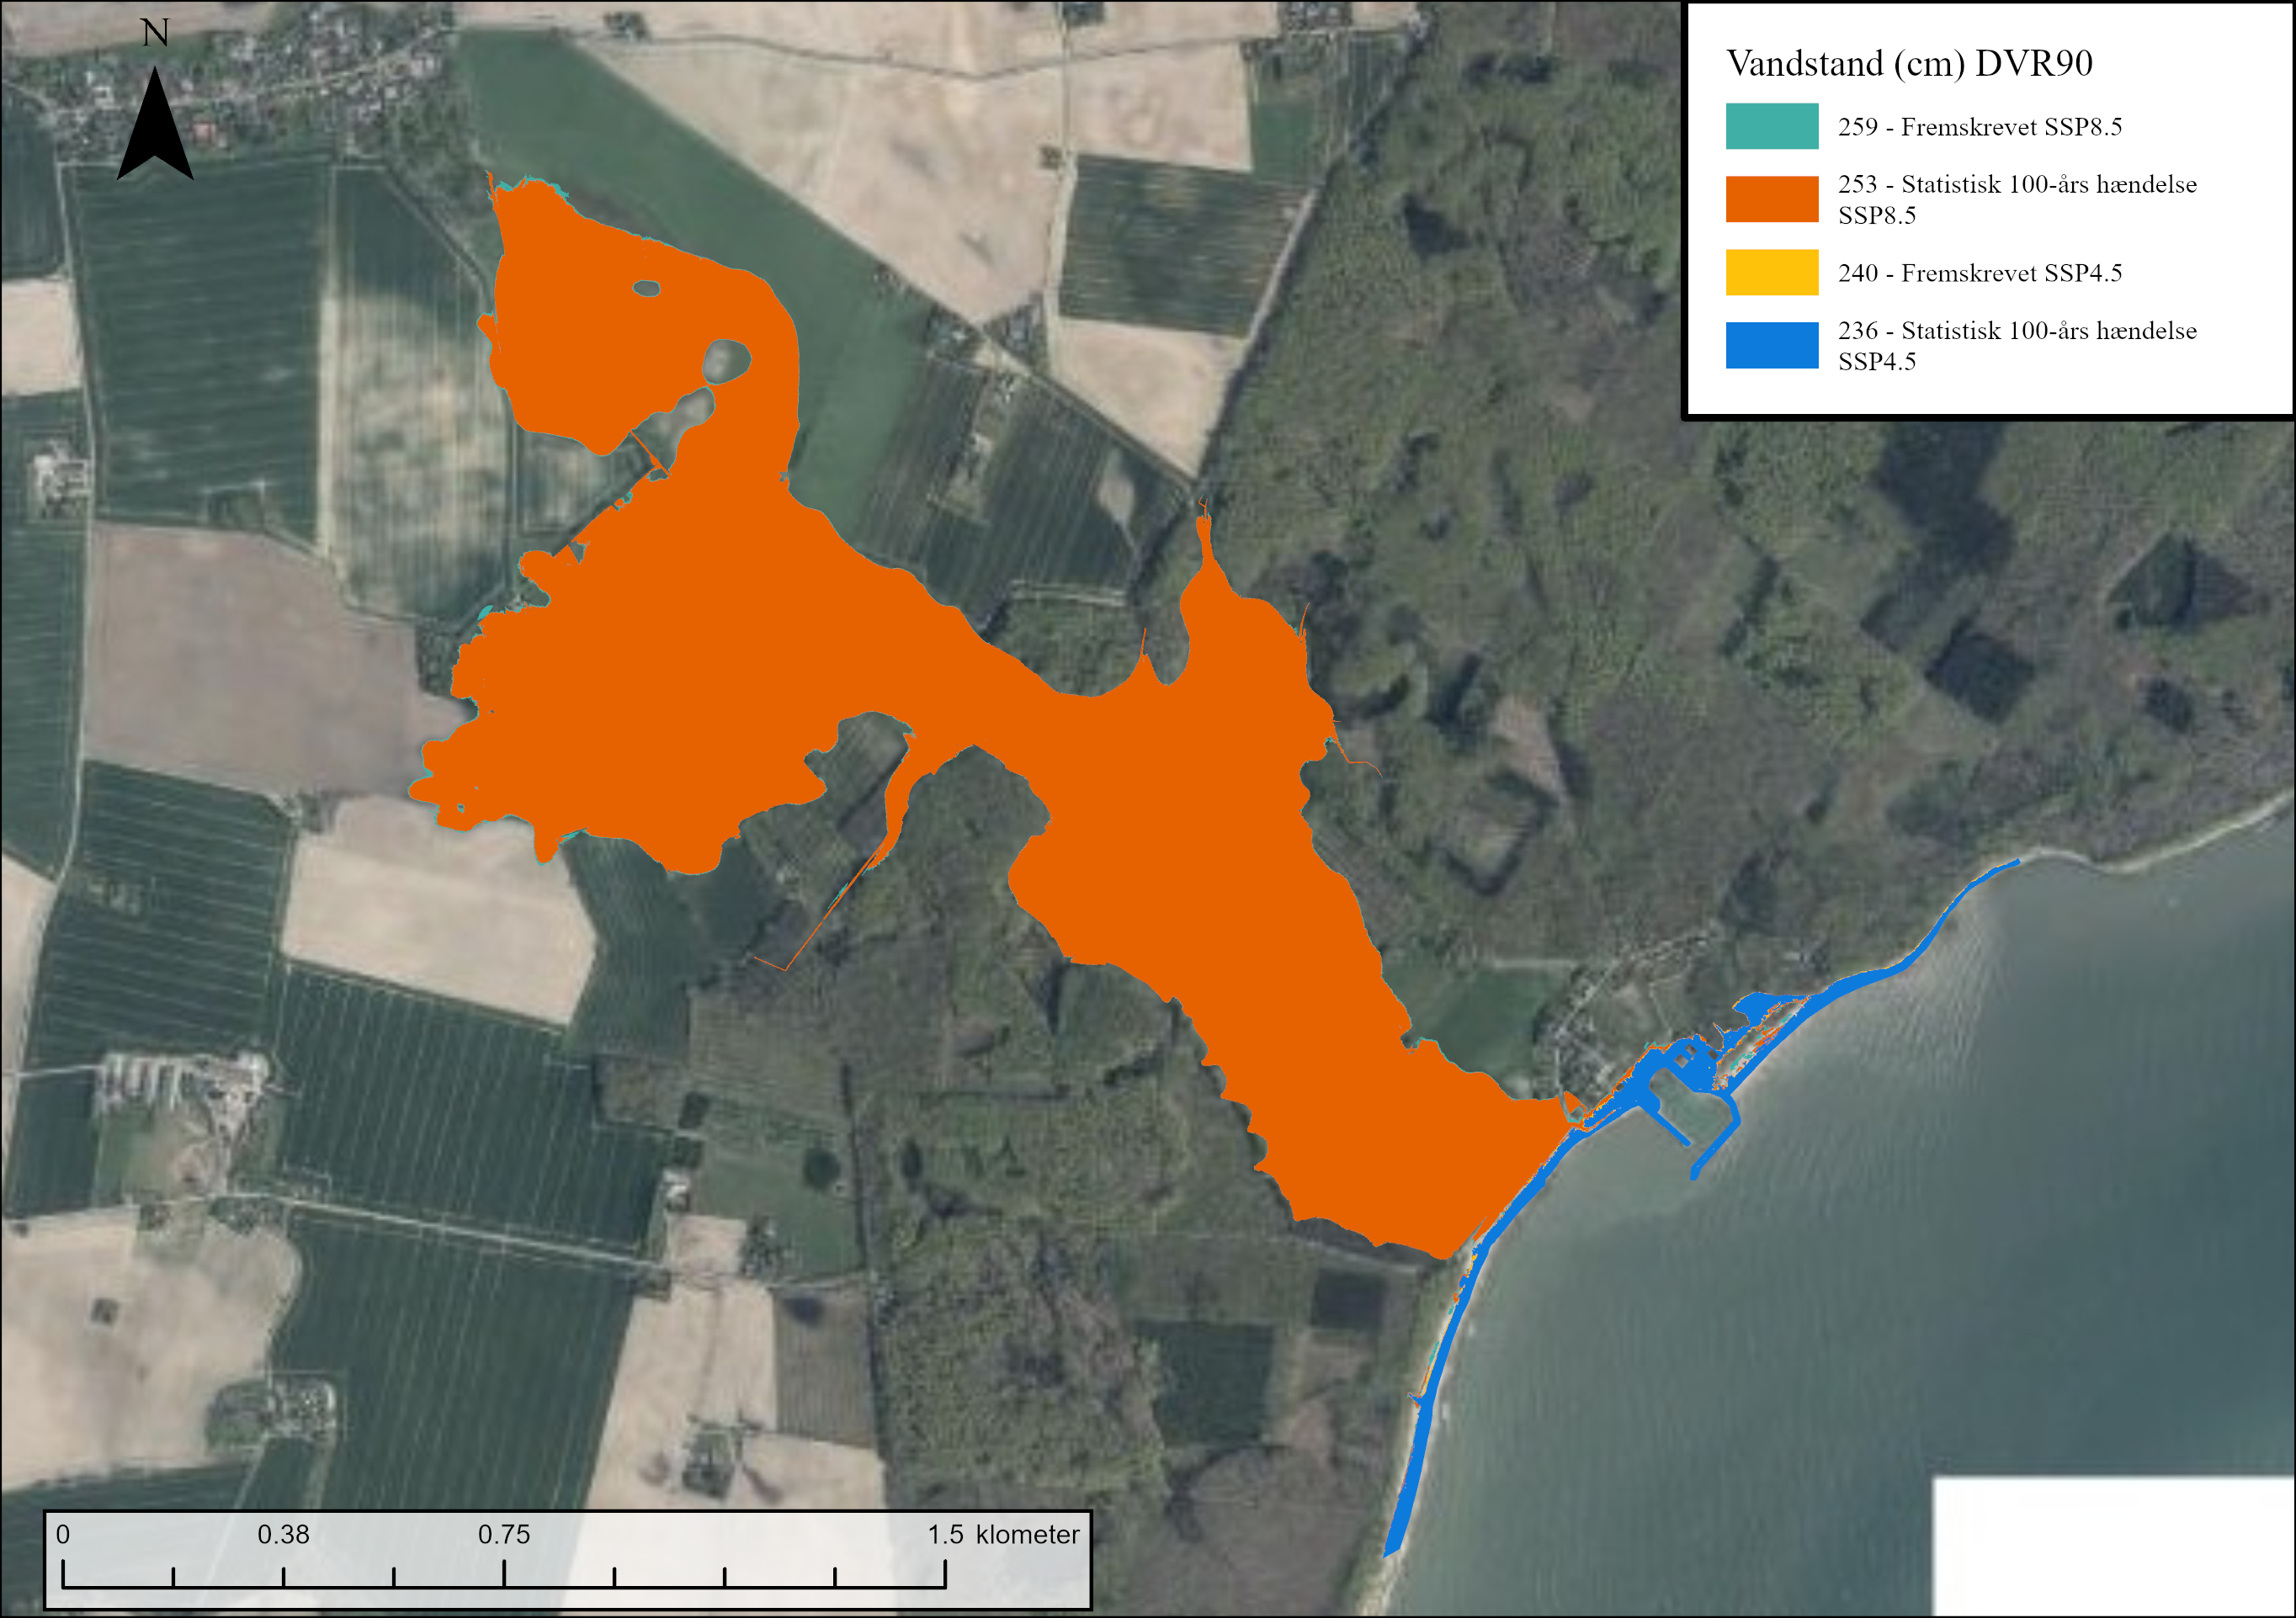
\includegraphics[width=0.8\linewidth]{images/Resultater/fremskrevet_hændelser/klima resultat hesnaes.jpg}
    \caption{Kort over oversvømmet areal i Hesnæs af en stormflod ved en statistisk 100-års hændelse og en fremskrivning af oktober 2023 stormfloden til slutningen af århundredet ved et SSP4,5 og SSP8,5 scenarie.}
    \label{Figur: Klima Hesnæs}
\end{figure}
I Hesnæs bliver et større lavliggende blandet græs- og landbrugsareal oversvømmet ved en 100-års hændelse i SSP8,5 scenariet. Ved en 100-års hændelse i SSP4,5 oversvømmes det meste af kysten og havnen. Selve Hesnæs by er udenfor oversvømmelsesrisiko selv ved det højeste vandstandsniveau på 259 cm DVR90 (figur \ref{Figur: Klima Hesnæs}). Ved en fremskrevet stormflod i SSP8,5, vil det oversvømmede areal stige fra 4,8 ha til 114,8 ha. Dette er en stigning på 2273\%. \\
Ved en fremskrevet 2023 stormflod ved SSP8,5 vil der oversvømmes et areal der er 3219\% større end det der blev målt under stormfloden i 2023. Dette er en stigning på 111 ha. \\

I figur \ref{Figur: Klima Præstø} ses vandets udbredelse ved en 100-års hændelse og en fremskrevet stormflod i et SSP4,5 og 8,5 scenarie for Præstø. Ved en 100-års SSP4,5 hændelse bliver dele af Præstø by oversvømmet, både nord og syd for Tubæk Ådal. Størstedelen af Tubæk Ådal vil også blive lagt under vand og åen vil gå over sine bredder i den sydlige del af byen. Ved vandstande på over 225 cm vil vandet følge Tubæk Å længere ind over land. Et areal der er 68\% større end stormfloden der oversvømmede byen i 2023 vil blive oversvømmet hvis den samme stormflod rammer Præstø i slutningen af dette århundrede i et SSP8,5 scenarie. Dette svarer til et 36 ha større oversvømmet areal.
\begin{figure}[H]
    \centering
    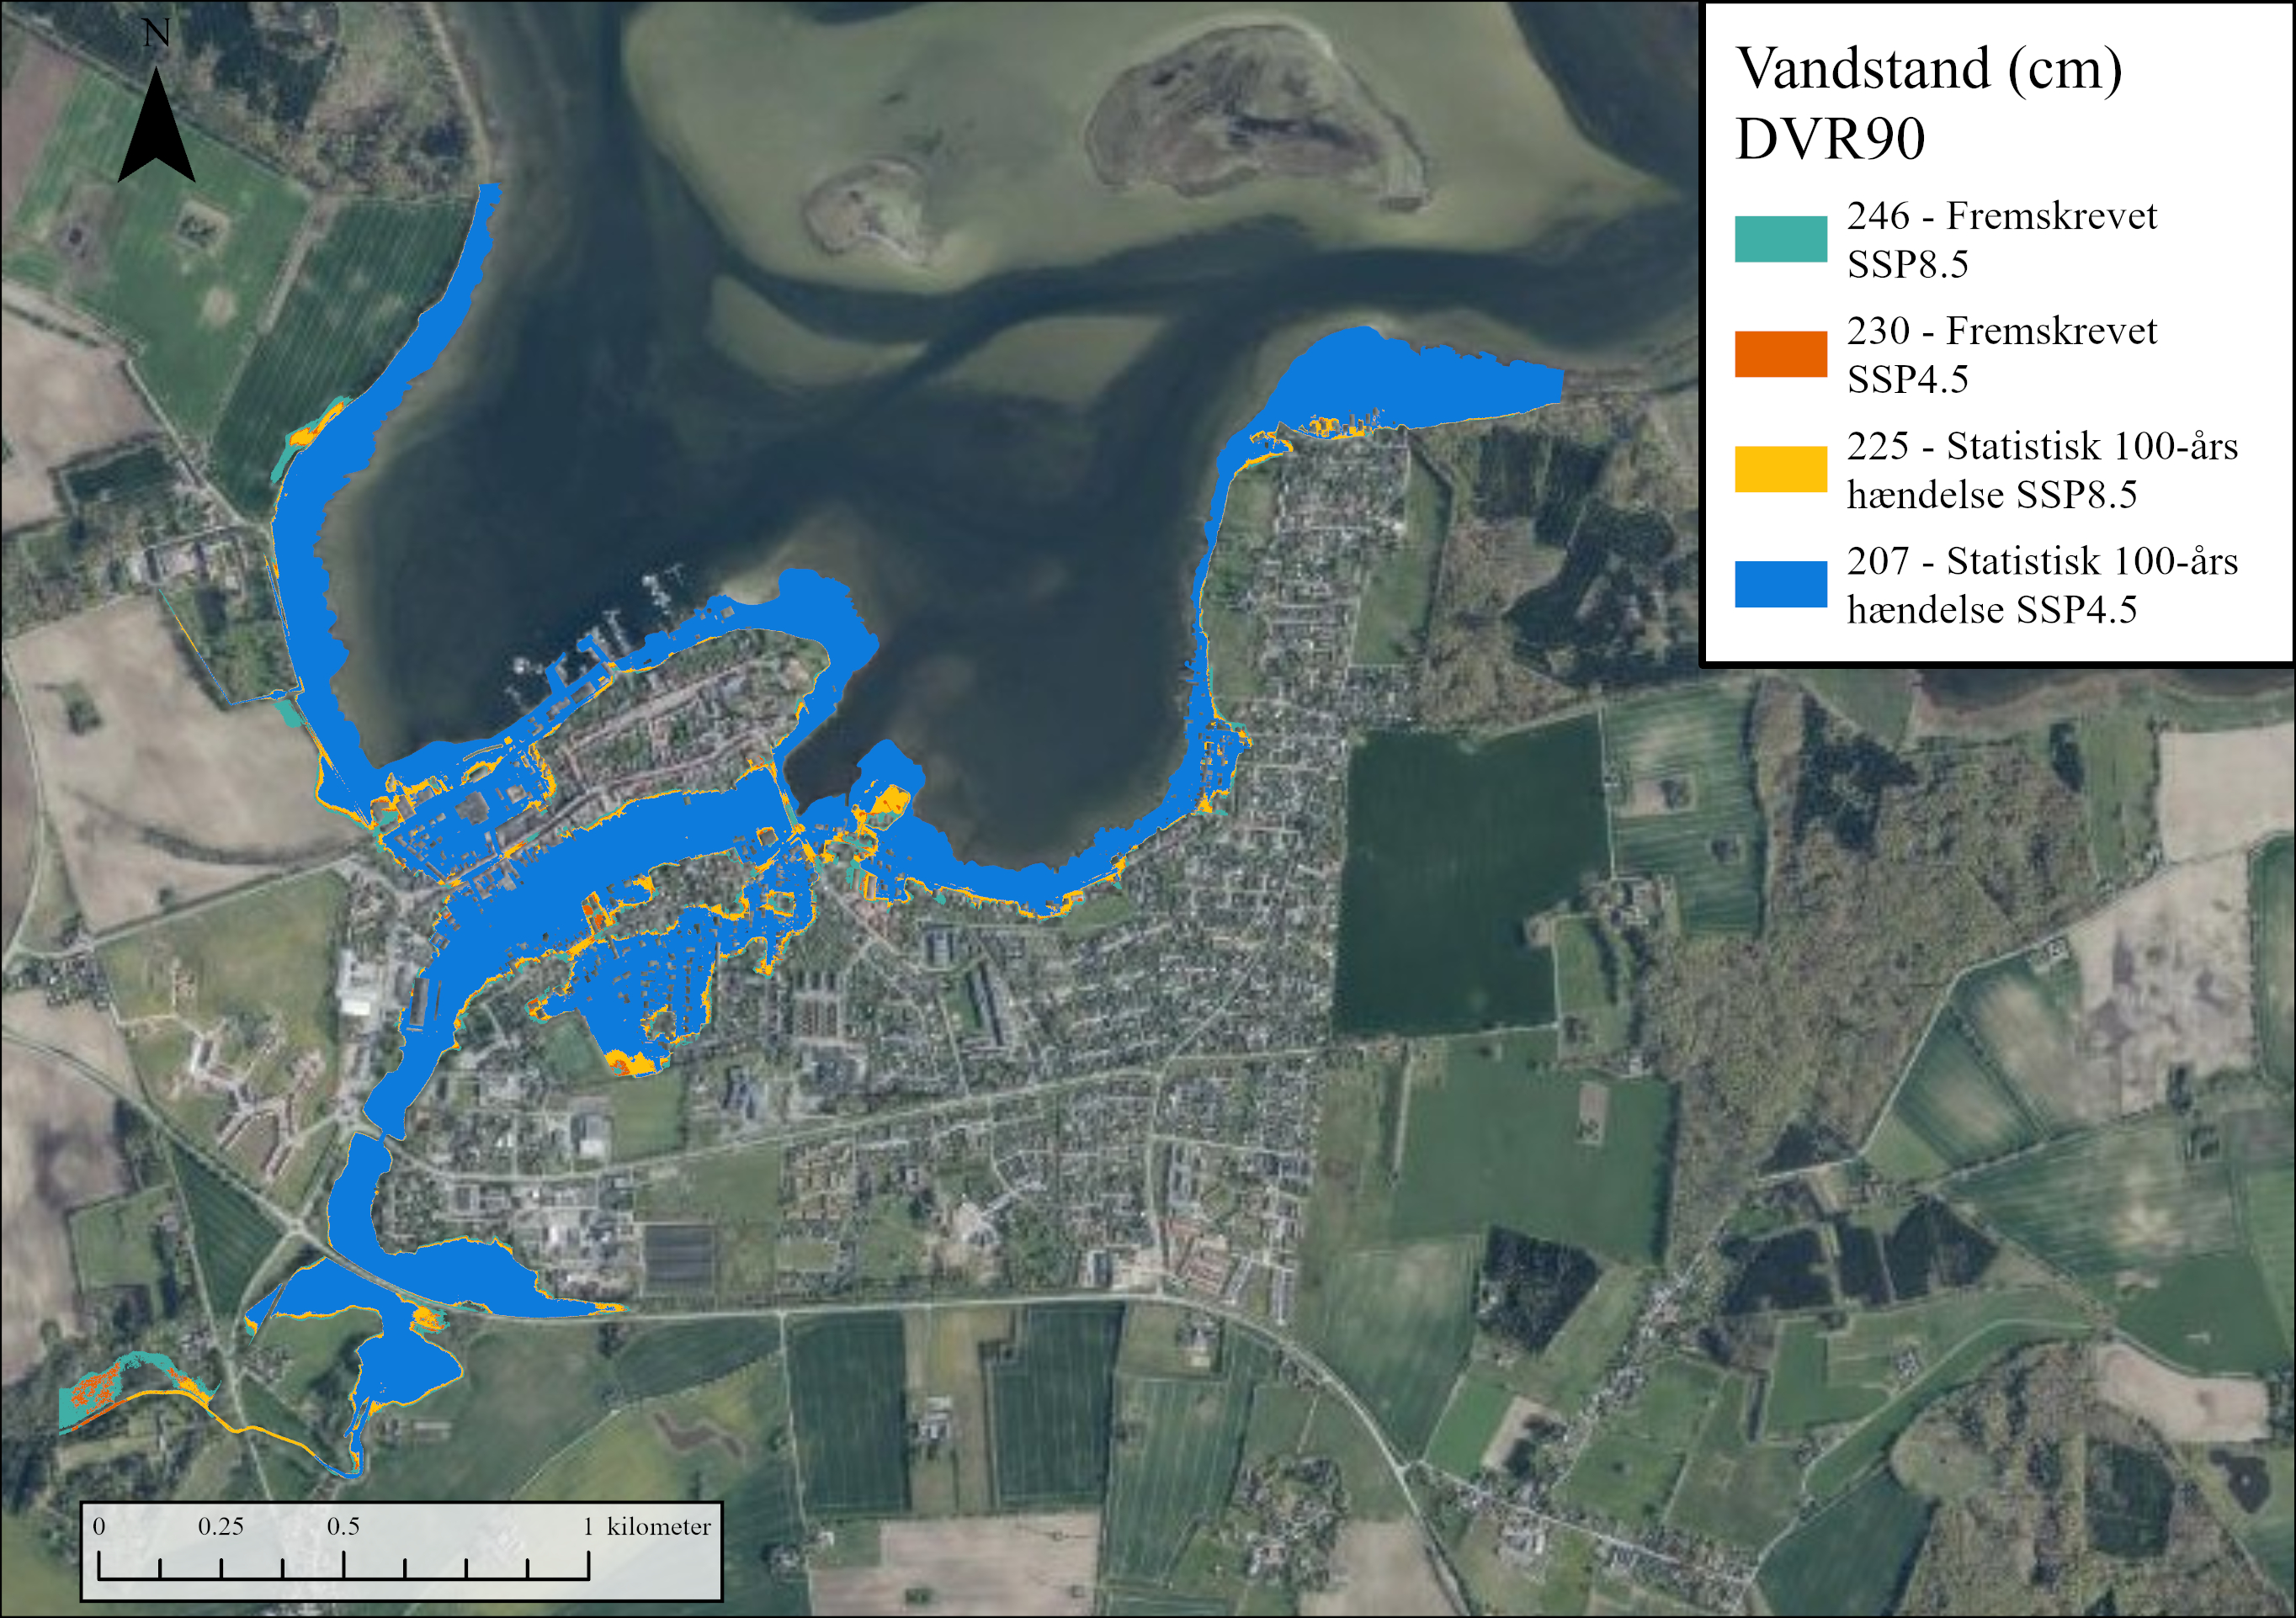
\includegraphics[width=0.8\linewidth]{images/Resultater/fremskrevet_hændelser/klima resultat praestoe.jpg}
    \caption{Kort over oversvømmet areal i Præstø af en stormflod ved en statistisk 100-års hændelse og en fremskrivning af oktober 2023 stormfloden til slutningen af århundredet ved et SSP4,5 og SSP8,5 scenarie.}
    \label{Figur: Klima Præstø}
\end{figure}
Sammenfattet bliver alle studieområderne påvirket af oversvømmelser ved stormfloder. I tabel \ref{Tabel: Oversvømmet arealer af stormfloder} er der blevet kvantificeret størrelsen af oversvømmelserne i hektar for alle hændelser simuleret af Inundation Modellen samt den observeret stormflod i 2023.\\ 
Det største oversvømmet areal er i Gedser Havn ved en fremskrevet 2023 stormflod i SSP8,5 på 219 ha og den mindste areal er simuleringen af 2023 stormfloden i Hesnæs på 3,3 ha. Gedser Havn er det område med den højeste absolutte stigning i oversvømmet areal med 186 ha fra den simuleret stormflod til en fremskrevet stormflod i SSP8,5. 
\begin{table}[H]
\centering
\renewcommand{\arraystretch}{1.2} 
\begin{threeparttable}
\caption{Oversvømmet areal af den observerede stormflod, den simuleret stormflod samt den statistiske 100-års hændelse og den fremskrevet stormflod til slutningen af århundredet ved SSP4.5 og 8.5 i hektar for hvert studieområde.}
    \begin{tabular}{@{} l S[table-format=3.1, output-decimal-marker={,}] 
                        S[table-format=3.1, output-decimal-marker={,}] 
                        S[table-format=3.1, output-decimal-marker={,}] 
                        S[table-format=3.1, output-decimal-marker={,}] 
                        S[table-format=3.1, output-decimal-marker={,}] 
                        S[table-format=3.1, output-decimal-marker={,}] @{}} 
    \toprule
    & \multicolumn{1}{c}{\textbf{\makecell{Observeret 2023\\stormflod}}} 
    & \multicolumn{1}{c}{\textbf{\makecell{Simuleret 2023\\stormflod}}} 
    & \multicolumn{2}{c}{\textbf{\makecell{Statistisk 100-års\\hændelse}}} 
    & \multicolumn{2}{c}{\textbf{\makecell{Fremskrevet 2023\\stormflod}}} \\ 
    \cmidrule(l){4-5} \cmidrule(l){6-7}
    {\textit{ha}} & & & {\textit{SSP4.5}} & {\textit{SSP8.5}} & {\textit{SSP4.5}} & {\textit{SSP8.5}} \\
    \midrule
      Aabenraa & 70,7 & 129,8 & 155,2 & 166,7 & 166,7 & 174,9 \\
      Gedser & 34,5 & 33,2 & 205,1 & 219,7 & 201 & 218,1 \\ 
      Hesnæs & 3.5 & 3,3 & 4,8 & 113,4 & 4,8 & 114,8 \\
      Præstø & 53,5 & 39,8 & 75,7 & 82 & 84,1 & 89,7 \\
    \bottomrule
    \end{tabular}
\label{Tabel: Oversvømmet arealer af stormfloder}
\end{threeparttable}
\end{table}


%\begin{table}[H]
%\centering
%\begin{threeparttable}
%\caption{Oversvømmet areal af den observeret 2023-stormflod, den simuleret 2023-stormflod samt den statistiske 100-års hændelse og den fremskrevet 2023-stormflod til slutningen af århundredet ved SSP4.5 og 8.5 i hektar og den procentvise forskel i forhold til 2023 stormfloden for hvert studieområde.}
%\begin{tabular}{@{} l >{\centering\arraybackslash}m{0.13\textwidth} >{\centering\arraybackslash}m{0.13\textwidth} >{\centering\arraybackslash}m{0.13\textwidth} >{\centering\arraybackslash}m{0.13\textwidth} >{\centering\arraybackslash}m{0.13\textwidth} >{\centering\arraybackslash}m{0.13\textwidth} @{}} 
%\toprule
%& \textbf{\makecell{Målt 2023\\stormflod}} 
%& \textbf{\makecell{Simuleret 2023\\stormflod}} 
%& \multicolumn{2}{c}{\textbf{\makecell{Statistisk 100-års\\hændelse}}} 
%& \multicolumn{2}{c}{\textbf{\makecell{Fremskrevet 2023\\stormflod}}} \\ 
%\cmidrule(l){4-5} \cmidrule(l){6-7}
%{\textit{ha}} & & & {\textit{SSP4.5}} & {\textit{SSP8.5}} & {\textit{SSP4.5}} & {\textit{SSP8.5}} \\
%\midrule
%\renewcommand{\arraystretch}{1.2}
%Aabenraa & 70,7 & 129,8 (+84\%) & 155,2 (+119\%) & 166,7 (+136\%) & 166,7 (+136\%) & 174,9 (+147\%)\\
%Gedser   & 34,5 & 33,2 (-4\%) & 205,1 (+495\%)& 219,7 (+537\%)& 201,0 (+483\%)& 218,1 (+533\%)\\ 
%Hesnæs   & 3,5  & 3,3 (-5\%) & 4,8 (+38\%)  & 113,4 (+3181\%) & 4,8 (+40\%) & 114,8 (+3220\%)\\
%Præstø   & 53,5 & 39,8 (-26\%)& 75,7 (+42\%)& 82,0 (+53\%)& 84,1 (+57\%)& 89,7 (+68\%)\\
%\bottomrule
%\end{tabular}
%\label{Tabel: Oversvømmet arealer af stormfloder i hektar}
%\end{threeparttable}
%\end{table}
 
\newpage
\section{Diskussion}


\section{Konklusion}


\newpage
\section{Referencer}
{\fontsize{11}{13} \selectfont \bibliography{references}}




\end{document}
